\PassOptionsToPackage{table}{xcolor}
\documentclass[9pt, aspectratio=169]{beamer}
% \documentclass[10pt]{beamer}
\usepackage[utf8]{inputenc}
\usepackage[T1]{fontenc}



\usepackage[table]{xcolor}
\usepackage[backend=biber, style=authoryear]{biblatex}
\addbibresource{local_references.bib}

%\usepackage{lmodern}
\usepackage{amsfonts,amssymb,amsmath}
\usetheme{Frankfurt}
% \useoutertheme[subsection=true]{miniframes}

% \useoutertheme[subsection=true]{miniframes}
\makeatletter
\let\beamer@writeslidentry@miniframeson=\beamer@writeslidentry
\def\beamer@writeslidentry@miniframesoff{%
  \expandafter\beamer@ifempty\expandafter{\beamer@framestartpage}{}% does not happen normally
  {%else
    % removed \addtocontents commands
    \clearpage\beamer@notesactions%
  }
}
\newcommand*{\miniframeson}{\let\beamer@writeslidentry=\beamer@writeslidentry@miniframeson}
\newcommand*{\miniframesoff}{\let\beamer@writeslidentry=\beamer@writeslidentry@miniframesoff}
\makeatother

\usepackage{multirow}
\usepackage{fontawesome5}


\usepackage{csquotes}
\usepackage[french]{babel}
\usepackage{csquotes}
\usepackage{setspace}
\usepackage{arydshln}

\usepackage{colortbl}
\usepackage{tabularx}
\renewcommand\tabularxcolumn[1]{m{#1}}

% --- Tickz
\usepackage{physics}
\usepackage{amsmath}
\usepackage{tikz}
\usepackage{mathdots}
\usepackage{yhmath}
\usepackage{cancel}
\usepackage{color}
\usepackage{siunitx}
\usepackage{array}
\usepackage{multirow}
\usepackage{amssymb}
\usepackage{gensymb}
\usepackage{tabularx}
\usepackage{extarrows}
\usepackage{booktabs}
\usetikzlibrary{fadings}
\usetikzlibrary{patterns}
\usetikzlibrary{shadows.blur}
\usetikzlibrary{shapes}

% ---------

\usepackage{booktabs}
\usepackage{setspace}
\usepackage{amssymb}
\usepackage{adjustbox}
\usepackage{pifont}
\usepackage[inkscapeformat=png]{svg}
\usepackage{graphicx}
\usepackage{times}
\setbeamertemplate{caption}[numbered]
% % \setbeamertemplate{bibliography item}{[\theenumiv]}

\setbeamerfont{bibliography item}{size=\tiny}
\setbeamerfont{bibliography entry author}{size=\tiny}
\setbeamerfont{bibliography entry title}{size=\tiny}
\setbeamerfont{bibliography entry location}{size=\tiny}
\setbeamerfont{bibliography entry note}{size=\tiny}

\setbeamerfont{frametitle}{size=\large}

\usepackage{caption}
\usepackage{float}
\usepackage{xcolor}
\usepackage{listings}
\usepackage{animate}

\definecolor{codegreen}{rgb}{0,0.6,0}
\definecolor{codegray}{rgb}{0.5,0.5,0.5}
\definecolor{codepurple}{rgb}{0.58,0,0.82}
\definecolor{backcolour}{rgb}{0.95,0.95,0.92}
 
\newcommand{\sensinterdit}{%
\tikz[baseline=-0.5ex]{
  \draw[red, line width=1pt, fill=red] (0,0) circle (0.8ex);
  \draw[white, line width=1pt] (-0.6ex,0) -- (0.6ex,0);
}}

\lstdefinestyle{mystyle}{
    backgroundcolor=\color{backcolour},   
    commentstyle=\color{codegreen},
    keywordstyle=\color{magenta},
    numberstyle=\tiny\color{codegray},
    stringstyle=\color{codepurple},
    basicstyle=\footnotesize,
    breakatwhitespace=false,         
    breaklines=true,                 
    captionpos=b,                    
    keepspaces=true,                 
    numbers=left,                    
    numbersep=5pt,                  
    showspaces=false,                
    showstringspaces=false,
    showtabs=false,                  
    tabsize=2
}
 
\lstset{style=mystyle}

\usepackage{ragged2e}
\setbeamercolor{section in foot}{fg=white,bg=darkorange}
\setbeamercolor{subsection in foot}{fg=white,bg=darkorange}
\setbeamercolor{frametitle}{fg=white, bg=darkorange}
\setbeamercolor{title}{fg=white, bg=darkorange}
\setbeamercolor{frame}{bg=darkorange}
\setbeamercolor{block title}{bg=darkorange,fg=white}

\setbeamercolor{item}{fg=darkorange}

% \definecolor{darkorange}{rgb}{0.81, 0.52, 0.05}
\definecolor{darkorange}{rgb}{1,0.5,0}
\definecolor{darkorange2}{rgb}{1, 0.64, 0.2}
\definecolor{honeydew}{rgb}{1, 0.85, 0.45}


\newenvironment{variableblock}[3]{%
  \setbeamercolor{block body}{#2}
  \setbeamercolor{block title}{#3}
  \begin{block}{#1}}{\end{block}}

\newenvironment{prosblock}[1]{%
  % \setbeamercolor{block body}{bg=blue,fg=white}
  \setbeamercolor{block title}{bg=blue,fg=white}
  \begin{block}{#1}}{\end{block}}

\newenvironment{consblock}[1]{%
  % \setbeamercolor{block body}{bg=red,fg=white}
  \setbeamercolor{block title}{bg=red,fg=white}
  \begin{block}{#1}}{\end{block}}

\newcommand{\cmark}{\ding{51}}%
\newcommand{\xmark}{\ding{55}}%

\renewcommand{\arraystretch}{1.5}
\newcommand{\vcentered}[1]{\raisebox{-.5\height}{#1}}

% Please add the following required packages to your document preamble:
\usepackage{booktabs}
\usepackage{multirow}
\usepackage{colortbl}
% Beamer presentation requires \usepackage{colortbl} instead of \usepackage[table,xcdraw]{xcolor}

\usepackage{tabularray}\UseTblrLibrary{varwidth}
\usepackage{xcolor}
\def\BibTeX{{\rm B\kern-.05em{\sc i\kern-.025em b}\kern-.08em
    T\kern-.1667em\lower.7ex\hbox{E}\kern-.125emX}}
% \usepackage{cite}
\usepackage{amsmath}
\newcommand{\probP}{\text{I\kern-0.15em P}}
\usepackage{etoolbox}
\patchcmd{\thebibliography}{\section*{\refname}}{}{}{}

\setlength\tabcolsep{0.5pt}

\renewcommand{\arraystretch}{0.9}
\setlength{\tabcolsep}{2pt}

\usepackage{pgffor}
\usepackage[absolute,overlay]{textpos}
\setlength{\TPHorizModule}{1cm}
\setlength{\TPVertModule}{1cm}

\setbeamerfont{bibliography item}{size=\tiny}
\setbeamerfont{bibliography entry author}{size=\tiny}
\setbeamerfont{bibliography entry title}{size=\tiny}
\setbeamerfont{bibliography entry location}{size=\tiny}
\setbeamerfont{bibliography entry note}{size=\tiny}

\setbeamerfont{bibliography entry author}{shape=\upshape,series=\mdseries,size=\footnotesize}
\setbeamerfont{bibliography entry title}{shape=\slshape,series=\mdseries,size=\footnotesize}
\setbeamerfont{bibliography entry journal}{shape=\upshape,series=\mdseries,size=\footnotesize}
\setbeamerfont{bibliography entry note}{shape=\upshape,series=\mdseries,size=\footnotesize}

\renewcommand*{\bibfont}{\scriptsize}

\newenvironment<>{varblock}[2][.9\textwidth]{%
  \setlength{\textwidth}{#1}
  \begin{actionenv}#3%
    \def\insertblocktitle{#2}%
    \par%
    \usebeamertemplate{block begin}}
  {\par%
    \usebeamertemplate{block end}%
  \end{actionenv}}

\newenvironment<>{alertvarblock}[2][.9\textwidth]{%
  \setlength{\textwidth}{#1}%
  \begin{actionenv}#3%
    \begin{alertblock}{#2}%
}{%
    \end{alertblock}%
  \end{actionenv}%
}

% \setbeamertemplate{footline}[frame number]

\setbeamertemplate{footline}{
  \leavevmode%
  \hfill
  \usebeamercolor[fg]{page number in head/foot}%
  \scriptsize%
  \ifnum\value{framenumber}>52%
    Appendix \number\numexpr\value{framenumber}-52\relax/53%
  \else%
    \ifnum\value{framenumber}>41%
      %
    \else
      \number\numexpr\value{framenumber}\relax/41%
    \fi

  \fi%
  \hspace{1em}
}


\begin{document}

\author{\textbf{Julien Soulé$^{1,2}$}, Jean-Paul Jamont$^1$, Michel Occello$^1$, Louis-Marie Traonouez$^2$, Paul Théron$^3$}

\title{\textbf{Towards Assisted MAS Design: A Library for
Explainable MARL with Organizational Model}}

\subtitle{ECAI 2024 Demo Presentation}

% \logo{\includegraphics[scale=0.01]{figures/grenoble-inp_logo.png}}

\institute{\footnotesize \textit{University Grenoble Alpes, Grenoble INP, LCIS, 26000, Valence, France \\
$^1$\{julien.soule, jean-paul.jamont, michel.occello\}@lcis.grenoble-inp.fr \\ \phantom{U} \\
Thales Land and Air Systems, BL IAS, 35000, Rennes, France \\
$^2$\{julien.soule, louis-marie.traonouez\}@thalesgroup.com \\ \phantom{U} \\
AICA IWG, La Guillermie, France \\
$^3$paul.theron@orange.fr}}


\date{\textit{\footnotesize May 9, 2024}}

%\subject{}
\setbeamercovered{transparent}
%\setbeamertemplate{navigation symbols}{}
\begin{frame}[plain]
	\maketitle\vspace{-0.8cm}
	\begin{figure}[ht!]
		\centering
            \includegraphics[height=0.8cm]{figures/la-ruche_logo.png}
            \hspace{0.8cm}
            \includegraphics[height=0.8cm]{figures/lcis_logo.png}
            \hspace{0.8cm}
		\includegraphics[height=0.8cm]{figures/grenoble-inp_logo.png}
            \hspace{0.8cm}
            \includegraphics[height=0.8cm]{figures/uga_logo.jpg}
	\end{figure}
\end{frame}

\addtocounter{framenumber}{-1}

\begin{frame}{Sommaire}
  \tableofcontents
\end{frame}

\section{Introduction}

% \AtBeginSection[]{
%   \begin{frame}
%     \frametitle{}
%     \tableofcontents[currentsection]
%   \end{frame}
% }

\begin{frame}{Introduction}{Contexte}

  \begin{columns}

    \begin{column}{0.7\textwidth}
      \begin{itemize}
        \item Augmentation \textbf{surface attaque} :
              \begin{itemize}
                \item Faiblesse IoT, Cloud\dots
                \item Contraintes temporelles, charge de travail, complexité\dots
                \item Brouillage, interruption de communication\dots
              \end{itemize}
      \end{itemize}
      $\Longrightarrow$ \textbf{Cyberdéfense} besoin de : \textbf{réactivité, flexibilité, autonomie}\dots

      \ \\

      \begin{itemize}
        \item \textit{\textbf{\textquote{Autonomous Intelligent Cyberdefense Agent} (AICA)}} \parencite{Kott2023}
              \begin{itemize}
                \item[$\Longrightarrow$] \textit{\textbf{\textquote{Multi-Agent System Centric AICA Reference Architecture}}} \parencite{theron2020mascara}
              \end{itemize}
              %   \item Détecter, identifier et caractériser les anomalies/attaques
              %   \item Planifier et exécuter des contre-mesures
              %   \item Être autonome, discret, interopérable, capable d'apprendre
      \end{itemize}

      \ \\

      $\Longrightarrow$ \textbf{Système Multi-Agent}\dots
      %
      \\[0.3cm]

      \hspace{3cm} \dots de \textbf{Cyberdéfense}
      %
      \\[0.4cm]

      \hspace{5cm} $\Longrightarrow$ \textbf{Organisation} des agents ?

    \end{column}

    \begin{column}{0.4\textwidth}
      \begin{figure}
        \includegraphics[width=\linewidth]{figures/casino.jpg}
        \caption*{\vspace{-0.5cm}\tiny\url{https://hackread.com/hackers-casinos-fish-tank-smart-thermometer-hack/}}
      \end{figure}

      \vspace{0.cm}
      \animategraphics[autoplay,loop,width=\linewidth]{1}{figures/cyberdefense_mas_frames/frame}{0}{8}

    \end{column}

  \end{columns}

\end{frame}

\begin{frame}{Introduction}{Problème}

  \begin{columns}

    \begin{column}{0.4\textwidth}
      \centering

      \begin{alertvarblock}[6cm]{Problème général}
        Quels \textbf{mécanismes organisationnels} du SMA de Cyberdéfense permettent d'\textbf{optimiser son fonctionnement} en tenant compte de ses \textbf{contraintes} ?
      \end{alertvarblock}

      \vspace{1em}

      \begin{itemize}
        \item \textbf{Recherche organisation adaptée}
              \begin{itemize}
                \item Contraintes environnementales
                \item Exigences de conception
              \end{itemize}

              \vspace{1em}

        \item \textbf{Mécanisme de recherche :}
              \begin{itemize}
                \item[(C1)] Autonomie
                \item [(C2)] Performance
                \item [(C3)] Adaptation
                \item [(C4)] Contrôle
                \item [(C5)] Explicabilité
              \end{itemize}
      \end{itemize}

    \end{column}

    \begin{column}{0.6\textwidth}
      % \resizebox{0.5\textwidth}{!}{
      \centering
      % \includegraphics[width=0.95\linewidth]{figures/general_problem_illustration.png}
      \vspace{0.1cm}
      \resizebox{1\linewidth}{!}{


\tikzset{every picture/.style={line width=0.75pt}} %set default line width to 0.75pt        

\begin{tikzpicture}[x=0.75pt,y=0.75pt,yscale=-1,xscale=1]
    %uncomment if require: \path (0,5804); %set diagram left start at 0, and has height of 5804

    %Shape: Rectangle [id:dp37204586795845374] 
    \draw   (15,4410) -- (660,4410) -- (660,5270) -- (15,5270) -- cycle ;
    %Shape: Rectangle [id:dp6528644209370597] 
    \draw   (40,4795) -- (271.14,4795) -- (271.14,4935) -- (40,4935) -- cycle ;
    %Shape: Rectangle [id:dp04838573396960488] 
    \draw  [fill={rgb, 255:red, 245; green, 166; blue, 35 }  ,fill opacity=1 ] (45,4804) .. controls (45,4801.79) and (46.79,4800) .. (49,4800) -- (101,4800) .. controls (103.21,4800) and (105,4801.79) .. (105,4804) -- (105,4826) .. controls (105,4828.21) and (103.21,4830) .. (101,4830) -- (49,4830) .. controls (46.79,4830) and (45,4828.21) .. (45,4826) -- cycle ;
    %Straight Lines [id:da28779803352593725] 
    % \draw    (105,4780) -- (125,4780) ;
    %Straight Lines [id:da9267919848430177] 
    \draw    (105,4865) -- (125,4865) ;
    %Straight Lines [id:da6747003832540825] 
    \draw    (185,4915) -- (205,4915) ;
    %Straight Lines [id:da42065693917376556] 
    \draw    (75,4880) -- (75,4900) ;
    %Straight Lines [id:da15025959978456238] 
    \draw    (155,4830) -- (155,4850) ;
    %Shape: Rectangle [id:dp04109612445272104] 
    \draw  [fill={rgb, 255:red, 126; green, 211; blue, 33 }  ,fill opacity=1 ] (125,4804) .. controls (125,4801.79) and (126.79,4800) .. (129,4800) -- (181,4800) .. controls (183.21,4800) and (185,4801.79) .. (185,4804) -- (185,4826) .. controls (185,4828.21) and (183.21,4830) .. (181,4830) -- (129,4830) .. controls (126.79,4830) and (125,4828.21) .. (125,4826) -- cycle ;
    %Shape: Rectangle [id:dp8218797438686123] 
    \draw  [fill={rgb, 255:red, 189; green, 16; blue, 224 }  ,fill opacity=1 ] (125,4854) .. controls (125,4851.79) and (126.79,4850) .. (129,4850) -- (181,4850) .. controls (183.21,4850) and (185,4851.79) .. (185,4854) -- (185,4876) .. controls (185,4878.21) and (183.21,4880) .. (181,4880) -- (129,4880) .. controls (126.79,4880) and (125,4878.21) .. (125,4876) -- cycle ;
    %Shape: Rectangle [id:dp37193948395169385] 
    \draw  [fill={rgb, 255:red, 184; green, 233; blue, 134 }  ,fill opacity=1 ] (45,4854) .. controls (45,4851.79) and (46.79,4850) .. (49,4850) -- (101,4850) .. controls (103.21,4850) and (105,4851.79) .. (105,4854) -- (105,4876) .. controls (105,4878.21) and (103.21,4880) .. (101,4880) -- (49,4880) .. controls (46.79,4880) and (45,4878.21) .. (45,4876) -- cycle ;
    %Straight Lines [id:da699052721095542] 
    \draw    (75,4830) -- (75,4850) ;
    %Shape: Rectangle [id:dp5056775522132636] 
    \draw  [fill={rgb, 255:red, 144; green, 19; blue, 254 }  ,fill opacity=1 ] (205,4804) .. controls (205,4801.79) and (206.79,4800) .. (209,4800) -- (261,4800) .. controls (263.21,4800) and (265,4801.79) .. (265,4804) -- (265,4876) .. controls (265,4878.21) and (263.21,4880) .. (261,4880) -- (209,4880) .. controls (206.79,4880) and (205,4878.21) .. (205,4876) -- cycle ;

    %Shape: Rectangle [id:dp5493685328045492] 
    \draw  [fill={rgb, 255:red, 208; green, 2; blue, 27 }  ,fill opacity=1 ] (45,4904) .. controls (45,4901.79) and (46.79,4900) .. (49,4900) -- (181,4900) .. controls (183.21,4900) and (185,4901.79) .. (185,4904) -- (185,4926) .. controls (185,4928.21) and (183.21,4930) .. (181,4930) -- (49,4930) .. controls (46.79,4930) and (45,4928.21) .. (45,4926) -- cycle ;
    %Straight Lines [id:da7074117972544659] 
    \draw    (155,4880) -- (155,4900) ;
    %Shape: Rectangle [id:dp32171767014290364] 
    \draw  [fill={rgb, 255:red, 80; green, 227; blue, 194 }  ,fill opacity=1 ] (205,4904) .. controls (205,4901.79) and (206.79,4900) .. (209,4900) -- (261,4900) .. controls (263.21,4900) and (265,4901.79) .. (265,4904) -- (265,4926) .. controls (265,4928.21) and (263.21,4930) .. (261,4930) -- (209,4930) .. controls (206.79,4930) and (205,4928.21) .. (205,4926) -- cycle ;
    %Straight Lines [id:da5336821600138906] 
    \draw    (235,4880) -- (235,4900) ;
    %Image [id:dp01351702105019581] 
    \draw (322.3,4872.5) node  {\includegraphics[width=18.44pt,height=18.75pt]{figures/cloud.png}};
    %Image [id:dp2893008276787382] 
    \draw (423.11,4905) node  {\includegraphics[width=14.75pt,height=15pt]{figures/server.png}};
    %Image [id:dp33084000544395364] 
    \draw (423.11,4870) node  {\includegraphics[width=14.75pt,height=15pt]{figures/server.png}};
    %Image [id:dp4045173494088059] 
    \draw (423.11,4835) node  {\includegraphics[width=14.75pt,height=15pt]{figures/server.png}};
    %Image [id:dp21670294007047108] 
    \draw (354.26,4870) node  {\includegraphics[width=14.75pt,height=15pt]{figures/11468565_brick_block_construction_build_wall_icon.png}};
    %Image [id:dp339375141118186] 
    \draw (457.54,4870) node  {\includegraphics[width=14.75pt,height=15pt]{figures/11468565_brick_block_construction_build_wall_icon.png}};
    %Image [id:dp8954911849692438] 
    \draw (388.69,4870) node  {\includegraphics[width=14.75pt,height=15pt]{figures/router.png}};
    %Image [id:dp6043253137812208] 
    \draw (491.97,4870) node  {\includegraphics[width=14.75pt,height=15pt]{figures/router.png}};
    %Image [id:dp5884883297493204] 
    \draw (565.74,4850) node  {\includegraphics[width=14.75pt,height=15pt]{figures/laptop.png}};
    %Image [id:dp08417059183927911] 
    \draw (600.16,4850) node  {\includegraphics[width=14.75pt,height=15pt]{figures/laptop.png}};
    %Image [id:dp7156849150132849] 
    \draw (600.16,4885) node  {\includegraphics[width=14.75pt,height=15pt]{figures/workstation.png}};
    %Image [id:dp6237848089278466] 
    \draw (565.74,4885) node  {\includegraphics[width=14.75pt,height=15pt]{figures/server.png}};
    %Image [id:dp7449851735440329] 
    \draw (531.31,4885) node  {\includegraphics[width=14.75pt,height=15pt]{figures/server.png}};
    %Image [id:dp005667224738301391] 
    \draw (531.31,4920) node  {\includegraphics[width=14.75pt,height=15pt]{figures/workstation.png}};
    %Image [id:dp8146427195897723] 
    \draw (565.74,4920) node  {\includegraphics[width=14.75pt,height=15pt]{figures/database.png}};
    %Image [id:dp49310370523635805] 
    \draw (600.16,4920) node  {\includegraphics[width=14.75pt,height=15pt]{figures/database.png}};
    %Image [id:dp020292600387318505] 
    \draw (531.31,4850) node  {\includegraphics[width=14.75pt,height=15pt]{figures/computer.png}};
    %Straight Lines [id:da2500380552659036] 
    \draw    (398.52,4870) -- (413.28,4870) ;
    %Straight Lines [id:da353449120783108] 
    \draw    (433.2,4870) -- (447.95,4870) ;
    %Straight Lines [id:da5004469875213738] 
    \draw    (467.38,4870) -- (482.13,4870) ;
    %Straight Lines [id:da6503894906953667] 
    \draw    (501.8,4870) -- (506.39,4870) -- (511.64,4870) ;
    %Straight Lines [id:da37401288462201976] 
    \draw    (511.64,4835) -- (511.64,4905) ;
    %Straight Lines [id:da5414293349526964] 
    \draw    (511.64,4870) -- (600.16,4870) ;
    %Straight Lines [id:da882160807467605] 
    \draw    (511.64,4835) -- (600.16,4835) ;
    %Straight Lines [id:da17424002654409498] 
    \draw    (511.64,4905) -- (600.16,4905) ;
    %Straight Lines [id:da974757219094287] 
    \draw    (531.31,4835) -- (531.31,4840) ;
    %Straight Lines [id:da12326774495407566] 
    \draw    (565.74,4835) -- (565.74,4840) ;
    %Straight Lines [id:da8825714625264635] 
    \draw    (600.16,4835) -- (600.16,4840) ;
    %Straight Lines [id:da8730507055269275] 
    \draw    (531.31,4870) -- (531.31,4875) ;
    %Straight Lines [id:da9685106023683034] 
    \draw    (565.74,4870) -- (565.74,4875) ;
    %Straight Lines [id:da6139098058213984] 
    \draw    (600.16,4870) -- (600.16,4875) ;
    %Straight Lines [id:da8488931299803314] 
    \draw    (531.31,4910) -- (531.31,4905) ;
    %Straight Lines [id:da48290744419465503] 
    \draw    (565.74,4910) -- (565.74,4905) ;
    %Straight Lines [id:da8004477536972611] 
    \draw    (600.16,4910) -- (600.16,4905) ;
    %Straight Lines [id:da25143467968820776] 
    \draw    (403.44,4835) -- (403.44,4905) ;
    %Straight Lines [id:da14951928183264374] 
    \draw    (442.79,4835) -- (442.79,4905) ;
    %Straight Lines [id:da9023759580794825] 
    \draw    (403.44,4835) -- (418.2,4835) ;
    %Straight Lines [id:da7547540666765368] 
    \draw    (432.95,4835) -- (442.79,4835) ;
    %Straight Lines [id:da050461431438784565] 
    \draw    (403.44,4905) -- (418.2,4905) ;
    %Straight Lines [id:da3825444784935419] 
    \draw    (432.95,4905) -- (442.79,4905) ;
    %Straight Lines [id:da8273733550666897] 
    \draw    (364.1,4870) -- (378.85,4870) ;
    %Straight Lines [id:da28397571787748854] 
    \draw    (329.67,4870) -- (344.43,4870) ;

    %Shape: Arc [id:dp5159031208901032] 
    \draw  [draw opacity=0] (296.48,5209.48) .. controls (296.48,5209.48) and (296.48,5209.48) .. (296.48,5209.48) .. controls (296.48,5209.48) and (296.48,5209.48) .. (296.48,5209.48) .. controls (298.29,5205.57) and (292.91,5199.13) .. (284.45,5195.11) .. controls (275.99,5191.08) and (267.66,5190.99) .. (265.84,5194.9) -- (281.16,5202.19) -- cycle ; \draw   (296.48,5209.48) .. controls (296.48,5209.48) and (296.48,5209.48) .. (296.48,5209.48) .. controls (296.48,5209.48) and (296.48,5209.48) .. (296.48,5209.48) .. controls (298.29,5205.57) and (292.91,5199.13) .. (284.45,5195.11) .. controls (275.99,5191.08) and (267.66,5190.99) .. (265.84,5194.9) ;
    %Shape: Arc [id:dp14312770217862503] 
    \draw  [draw opacity=0] (292.1,5213.16) .. controls (292.1,5213.16) and (292.1,5213.16) .. (292.1,5213.16) .. controls (293.91,5209.25) and (289.51,5203.28) .. (282.26,5199.83) .. controls (275.01,5196.38) and (267.66,5196.75) .. (265.84,5200.66) -- (278.97,5206.91) -- cycle ; \draw   (292.1,5213.16) .. controls (292.1,5213.16) and (292.1,5213.16) .. (292.1,5213.16) .. controls (293.91,5209.25) and (289.51,5203.28) .. (282.26,5199.83) .. controls (275.01,5196.38) and (267.66,5196.75) .. (265.84,5200.66) ;
    %Shape: Arc [id:dp10841807511888646] 
    \draw  [draw opacity=0] (287.71,5216.84) .. controls (289.53,5212.93) and (286.11,5207.43) .. (280.06,5204.55) .. controls (274.02,5201.68) and (267.65,5202.52) .. (265.83,5206.43) -- (276.77,5211.64) -- cycle ; \draw   (287.71,5216.84) .. controls (289.53,5212.93) and (286.11,5207.43) .. (280.06,5204.55) .. controls (274.02,5201.68) and (267.65,5202.52) .. (265.83,5206.43) ;
    %Shape: Arc [id:dp5497029665203269] 
    \draw  [draw opacity=0] (283.33,5220.52) .. controls (283.33,5220.52) and (283.33,5220.52) .. (283.33,5220.52) .. controls (285.15,5216.61) and (282.7,5211.58) .. (277.87,5209.28) .. controls (273.04,5206.97) and (267.64,5208.28) .. (265.83,5212.19) -- (274.58,5216.36) -- cycle ; \draw   (283.33,5220.52) .. controls (283.33,5220.52) and (283.33,5220.52) .. (283.33,5220.52) .. controls (285.15,5216.61) and (282.7,5211.58) .. (277.87,5209.28) .. controls (273.04,5206.97) and (267.64,5208.28) .. (265.83,5212.19) ;
    %Shape: Arc [id:dp9043594701708034] 
    \draw  [draw opacity=0] (278.95,5224.21) .. controls (278.95,5224.21) and (278.95,5224.21) .. (278.95,5224.21) .. controls (280.77,5220.29) and (279.3,5215.72) .. (275.68,5214) .. controls (272.05,5212.27) and (267.64,5214.05) .. (265.82,5217.96) -- (272.39,5221.08) -- cycle ; \draw   (278.95,5224.21) .. controls (278.95,5224.21) and (278.95,5224.21) .. (278.95,5224.21) .. controls (280.77,5220.29) and (279.3,5215.72) .. (275.68,5214) .. controls (272.05,5212.27) and (267.64,5214.05) .. (265.82,5217.96) ;

    %Shape: Smiley Face [id:dp410186171361024] 
    \draw  [line width=1.5]  (274.77,5238.14) .. controls (274.77,5231.59) and (269.23,5226.28) .. (262.39,5226.28) .. controls (255.55,5226.28) and (250,5231.59) .. (250,5238.14) .. controls (250,5244.69) and (255.55,5250) .. (262.39,5250) .. controls (269.23,5250) and (274.77,5244.69) .. (274.77,5238.14) -- cycle ; \draw  [line width=1.5]  (267.84,5234.11) .. controls (267.84,5233.45) and (267.28,5232.92) .. (266.6,5232.92) .. controls (265.91,5232.92) and (265.36,5233.45) .. (265.36,5234.11) .. controls (265.36,5234.76) and (265.91,5235.29) .. (266.6,5235.29) .. controls (267.28,5235.29) and (267.84,5234.76) .. (267.84,5234.11) -- cycle ; \draw  [line width=1.5]  (259.41,5234.11) .. controls (259.41,5233.45) and (258.86,5232.92) .. (258.17,5232.92) .. controls (257.49,5232.92) and (256.94,5233.45) .. (256.94,5234.11) .. controls (256.94,5234.76) and (257.49,5235.29) .. (258.17,5235.29) .. controls (258.86,5235.29) and (259.41,5234.76) .. (259.41,5234.11) -- cycle ; \draw  [line width=1.5]  (268.58,5242.88) .. controls (264.45,5246.05) and (260.32,5246.05) .. (256.19,5242.88) ;
    %Shape: Smiley Face [id:dp6297513983610752] 
    \draw  [line width=1.5]  (244.99,5126.86) .. controls (244.99,5120.31) and (250.59,5115) .. (257.5,5115) .. controls (264.4,5115) and (270,5120.31) .. (270,5126.86) .. controls (270,5133.41) and (264.4,5138.72) .. (257.5,5138.72) .. controls (250.59,5138.72) and (244.99,5133.41) .. (244.99,5126.86) -- cycle ; \draw  [line width=1.5]  (252,5122.83) .. controls (252,5122.17) and (252.56,5121.64) .. (253.25,5121.64) .. controls (253.94,5121.64) and (254.5,5122.17) .. (254.5,5122.83) .. controls (254.5,5123.48) and (253.94,5124.01) .. (253.25,5124.01) .. controls (252.56,5124.01) and (252,5123.48) .. (252,5122.83) -- cycle ; \draw  [line width=1.5]  (260.5,5122.83) .. controls (260.5,5122.17) and (261.06,5121.64) .. (261.75,5121.64) .. controls (262.44,5121.64) and (263,5122.17) .. (263,5122.83) .. controls (263,5123.48) and (262.44,5124.01) .. (261.75,5124.01) .. controls (261.06,5124.01) and (260.5,5123.48) .. (260.5,5122.83) -- cycle ; \draw  [line width=1.5]  (251.25,5131.6) .. controls (255.41,5134.77) and (259.58,5134.77) .. (263.75,5131.6) ;
    %Shape: Smiley Face [id:dp4180730149094508] 
    \draw  [line width=1.5]  (426.61,5136.15) .. controls (426.61,5129.6) and (432.2,5124.29) .. (439.11,5124.29) .. controls (446.01,5124.29) and (451.61,5129.6) .. (451.61,5136.15) .. controls (451.61,5142.69) and (446.01,5148) .. (439.11,5148) .. controls (432.2,5148) and (426.61,5142.69) .. (426.61,5136.15) -- cycle ; \draw  [line width=1.5]  (433.61,5132.11) .. controls (433.61,5131.46) and (434.17,5130.93) .. (434.86,5130.93) .. controls (435.55,5130.93) and (436.11,5131.46) .. (436.11,5132.11) .. controls (436.11,5132.77) and (435.55,5133.3) .. (434.86,5133.3) .. controls (434.17,5133.3) and (433.61,5132.77) .. (433.61,5132.11) -- cycle ; \draw  [line width=1.5]  (442.11,5132.11) .. controls (442.11,5131.46) and (442.67,5130.93) .. (443.36,5130.93) .. controls (444.05,5130.93) and (444.61,5131.46) .. (444.61,5132.11) .. controls (444.61,5132.77) and (444.05,5133.3) .. (443.36,5133.3) .. controls (442.67,5133.3) and (442.11,5132.77) .. (442.11,5132.11) -- cycle ; \draw  [line width=1.5]  (432.86,5140.89) .. controls (437.02,5144.05) and (441.19,5144.05) .. (445.36,5140.89) ;
    %Shape: Arc [id:dp026164586189738936] 
    \draw  [draw opacity=0] (298.04,5128.6) .. controls (298.04,5128.6) and (298.04,5128.6) .. (298.04,5128.6) .. controls (298.04,5128.6) and (298.04,5128.6) .. (298.04,5128.6) .. controls (301.88,5130.63) and (301.47,5139.01) .. (297.12,5147.32) .. controls (292.77,5155.63) and (286.13,5160.72) .. (282.28,5158.69) -- (290.16,5143.64) -- cycle ; \draw   (298.04,5128.6) .. controls (298.04,5128.6) and (298.04,5128.6) .. (298.04,5128.6) .. controls (298.04,5128.6) and (298.04,5128.6) .. (298.04,5128.6) .. controls (301.88,5130.63) and (301.47,5139.01) .. (297.12,5147.32) .. controls (292.77,5155.63) and (286.13,5160.72) .. (282.28,5158.69) ;
    %Shape: Arc [id:dp21730922944992026] 
    \draw  [draw opacity=0] (292.27,5128.3) .. controls (292.27,5128.3) and (292.27,5128.3) .. (292.27,5128.3) .. controls (296.11,5130.33) and (296.21,5137.75) .. (292.48,5144.87) .. controls (288.75,5151.99) and (282.61,5156.12) .. (278.77,5154.09) -- (285.52,5141.19) -- cycle ; \draw   (292.27,5128.3) .. controls (292.27,5128.3) and (292.27,5128.3) .. (292.27,5128.3) .. controls (296.11,5130.33) and (296.21,5137.75) .. (292.48,5144.87) .. controls (288.75,5151.99) and (282.61,5156.12) .. (278.77,5154.09) ;
    %Shape: Arc [id:dp8745570103378975] 
    \draw  [draw opacity=0] (286.5,5128) .. controls (290.35,5130.03) and (290.95,5136.48) .. (287.84,5142.42) .. controls (284.73,5148.35) and (279.1,5151.52) .. (275.25,5149.49) -- (280.87,5138.74) -- cycle ; \draw   (286.5,5128) .. controls (290.35,5130.03) and (290.95,5136.48) .. (287.84,5142.42) .. controls (284.73,5148.35) and (279.1,5151.52) .. (275.25,5149.49) ;
    %Shape: Arc [id:dp32428917068964835] 
    \draw  [draw opacity=0] (280.73,5127.7) .. controls (280.73,5127.7) and (280.73,5127.7) .. (280.73,5127.7) .. controls (284.58,5129.73) and (285.68,5135.22) .. (283.2,5139.97) .. controls (280.71,5144.72) and (275.58,5146.92) .. (271.73,5144.89) -- (276.23,5136.29) -- cycle ; \draw   (280.73,5127.7) .. controls (280.73,5127.7) and (280.73,5127.7) .. (280.73,5127.7) .. controls (284.58,5129.73) and (285.68,5135.22) .. (283.2,5139.97) .. controls (280.71,5144.72) and (275.58,5146.92) .. (271.73,5144.89) ;
    %Shape: Arc [id:dp1721423421834739] 
    \draw  [draw opacity=0] (274.96,5127.39) .. controls (278.81,5129.42) and (280.42,5133.96) .. (278.55,5137.52) .. controls (276.69,5141.08) and (272.06,5142.32) .. (268.21,5140.29) .. controls (268.21,5140.29) and (268.21,5140.29) .. (268.21,5140.29) -- (271.59,5133.84) -- cycle ; \draw   (274.96,5127.39) .. controls (278.81,5129.42) and (280.42,5133.96) .. (278.55,5137.52) .. controls (276.69,5141.08) and (272.06,5142.32) .. (268.21,5140.29) .. controls (268.21,5140.29) and (268.21,5140.29) .. (268.21,5140.29) ;

    %Shape: Arc [id:dp5844771861273294] 
    \draw  [draw opacity=0] (401.71,5157.34) .. controls (401.71,5157.34) and (401.71,5157.34) .. (401.71,5157.34) .. controls (401.71,5157.34) and (401.71,5157.34) .. (401.71,5157.34) .. controls (397.38,5157.78) and (393,5150.6) .. (391.93,5141.29) .. controls (390.87,5131.98) and (393.51,5124.07) .. (397.84,5123.63) -- (399.78,5140.48) -- cycle ; \draw   (401.71,5157.34) .. controls (401.71,5157.34) and (401.71,5157.34) .. (401.71,5157.34) .. controls (401.71,5157.34) and (401.71,5157.34) .. (401.71,5157.34) .. controls (397.38,5157.78) and (393,5150.6) .. (391.93,5141.29) .. controls (390.87,5131.98) and (393.51,5124.07) .. (397.84,5123.63) ;
    %Shape: Arc [id:dp15304922541241428] 
    \draw  [draw opacity=0] (406.66,5154.39) .. controls (402.33,5154.83) and (398.07,5148.73) .. (397.16,5140.75) .. controls (396.25,5132.77) and (399.02,5125.94) .. (403.35,5125.49) -- (405,5139.94) -- cycle ; \draw   (406.66,5154.39) .. controls (402.33,5154.83) and (398.07,5148.73) .. (397.16,5140.75) .. controls (396.25,5132.77) and (399.02,5125.94) .. (403.35,5125.49) ;
    %Shape: Arc [id:dp5873695783447137] 
    \draw  [draw opacity=0] (411.61,5151.44) .. controls (407.28,5151.89) and (403.15,5146.86) .. (402.39,5140.21) .. controls (401.63,5133.56) and (404.52,5127.81) .. (408.85,5127.36) -- (410.23,5139.4) -- cycle ; \draw   (411.61,5151.44) .. controls (407.28,5151.89) and (403.15,5146.86) .. (402.39,5140.21) .. controls (401.63,5133.56) and (404.52,5127.81) .. (408.85,5127.36) ;
    %Shape: Arc [id:dp3340412252291639] 
    \draw  [draw opacity=0] (416.56,5148.49) .. controls (416.56,5148.49) and (416.56,5148.49) .. (416.56,5148.49) .. controls (412.23,5148.94) and (408.23,5144.99) .. (407.62,5139.67) .. controls (407.01,5134.35) and (410.02,5129.68) .. (414.35,5129.23) -- (415.46,5138.86) -- cycle ; \draw   (416.56,5148.49) .. controls (416.56,5148.49) and (416.56,5148.49) .. (416.56,5148.49) .. controls (412.23,5148.94) and (408.23,5144.99) .. (407.62,5139.67) .. controls (407.01,5134.35) and (410.02,5129.68) .. (414.35,5129.23) ;
    %Shape: Arc [id:dp8319335091648151] 
    \draw  [draw opacity=0] (421.51,5145.54) .. controls (421.51,5145.54) and (421.51,5145.54) .. (421.51,5145.54) .. controls (417.18,5145.99) and (413.3,5143.12) .. (412.84,5139.13) .. controls (412.39,5135.14) and (415.53,5131.54) .. (419.86,5131.1) -- (420.69,5138.32) -- cycle ; \draw   (421.51,5145.54) .. controls (421.51,5145.54) and (421.51,5145.54) .. (421.51,5145.54) .. controls (417.18,5145.99) and (413.3,5143.12) .. (412.84,5139.13) .. controls (412.39,5135.14) and (415.53,5131.54) .. (419.86,5131.1) ;

    %Shape: Arc [id:dp8902921027407593] 
    \draw  [draw opacity=0] (443.09,5184.48) .. controls (441.25,5180.57) and (446.69,5174.13) .. (455.23,5170.11) .. controls (463.76,5166.08) and (472.17,5165.99) .. (474.01,5169.9) .. controls (474.01,5169.9) and (474.01,5169.9) .. (474.01,5169.9) -- (458.55,5177.19) -- cycle ; \draw   (443.09,5184.48) .. controls (441.25,5180.57) and (446.69,5174.13) .. (455.23,5170.11) .. controls (463.76,5166.08) and (472.17,5165.99) .. (474.01,5169.9) .. controls (474.01,5169.9) and (474.01,5169.9) .. (474.01,5169.9) ;
    %Shape: Arc [id:dp27157954351388136] 
    \draw  [draw opacity=0] (447.51,5188.17) .. controls (447.51,5188.17) and (447.51,5188.17) .. (447.51,5188.17) .. controls (445.68,5184.25) and (450.12,5178.28) .. (457.44,5174.83) .. controls (464.76,5171.38) and (472.18,5171.75) .. (474.01,5175.67) -- (460.76,5181.92) -- cycle ; \draw   (447.51,5188.17) .. controls (447.51,5188.17) and (447.51,5188.17) .. (447.51,5188.17) .. controls (445.68,5184.25) and (450.12,5178.28) .. (457.44,5174.83) .. controls (464.76,5171.38) and (472.18,5171.75) .. (474.01,5175.67) ;
    %Shape: Arc [id:dp24024767983904605] 
    \draw  [draw opacity=0] (451.93,5191.85) .. controls (451.93,5191.85) and (451.93,5191.85) .. (451.93,5191.85) .. controls (450.1,5187.93) and (453.55,5182.43) .. (459.65,5179.55) .. controls (465.75,5176.68) and (472.18,5177.52) .. (474.02,5181.43) -- (462.97,5186.64) -- cycle ; \draw   (451.93,5191.85) .. controls (451.93,5191.85) and (451.93,5191.85) .. (451.93,5191.85) .. controls (450.1,5187.93) and (453.55,5182.43) .. (459.65,5179.55) .. controls (465.75,5176.68) and (472.18,5177.52) .. (474.02,5181.43) ;
    %Shape: Arc [id:dp20091537172617546] 
    \draw  [draw opacity=0] (456.35,5195.53) .. controls (456.35,5195.53) and (456.35,5195.53) .. (456.35,5195.53) .. controls (454.52,5191.62) and (456.99,5186.58) .. (461.87,5184.28) .. controls (466.75,5181.98) and (472.19,5183.28) .. (474.02,5187.2) -- (465.19,5191.36) -- cycle ; \draw   (456.35,5195.53) .. controls (456.35,5195.53) and (456.35,5195.53) .. (456.35,5195.53) .. controls (454.52,5191.62) and (456.99,5186.58) .. (461.87,5184.28) .. controls (466.75,5181.98) and (472.19,5183.28) .. (474.02,5187.2) ;
    %Shape: Arc [id:dp5171323467750554] 
    \draw  [draw opacity=0] (460.78,5199.21) .. controls (458.94,5195.3) and (460.42,5190.73) .. (464.08,5189) .. controls (467.74,5187.28) and (472.19,5189.05) .. (474.03,5192.96) -- (467.4,5196.09) -- cycle ; \draw   (460.78,5199.21) .. controls (458.94,5195.3) and (460.42,5190.73) .. (464.08,5189) .. controls (467.74,5187.28) and (472.19,5189.05) .. (474.03,5192.96) ;

    %Shape: Smiley Face [id:dp8410574975235354] 
    \draw  [line width=1.5]  (464.99,5213.14) .. controls (464.99,5206.59) and (470.59,5201.29) .. (477.5,5201.29) .. controls (484.4,5201.29) and (490,5206.59) .. (490,5213.14) .. controls (490,5219.69) and (484.4,5225) .. (477.5,5225) .. controls (470.59,5225) and (464.99,5219.69) .. (464.99,5213.14) -- cycle ; \draw  [line width=1.5]  (472,5209.11) .. controls (472,5208.46) and (472.56,5207.93) .. (473.25,5207.93) .. controls (473.94,5207.93) and (474.5,5208.46) .. (474.5,5209.11) .. controls (474.5,5209.77) and (473.94,5210.3) .. (473.25,5210.3) .. controls (472.56,5210.3) and (472,5209.77) .. (472,5209.11) -- cycle ; \draw  [line width=1.5]  (480.5,5209.11) .. controls (480.5,5208.46) and (481.06,5207.93) .. (481.75,5207.93) .. controls (482.44,5207.93) and (483,5208.46) .. (483,5209.11) .. controls (483,5209.77) and (482.44,5210.3) .. (481.75,5210.3) .. controls (481.06,5210.3) and (480.5,5209.77) .. (480.5,5209.11) -- cycle ; \draw  [line width=1.5]  (471.25,5217.89) .. controls (475.41,5221.05) and (479.58,5221.05) .. (483.75,5217.89) ;
    %Shape: Smiley Face [id:dp9549925896715118] 
    \draw  [line width=1.5]  (374.99,5215.96) .. controls (374.99,5209.41) and (380.59,5204.1) .. (387.5,5204.1) .. controls (394.4,5204.1) and (400,5209.41) .. (400,5215.96) .. controls (400,5222.51) and (394.4,5227.82) .. (387.5,5227.82) .. controls (380.59,5227.82) and (374.99,5222.51) .. (374.99,5215.96) -- cycle ; \draw  [line width=1.5]  (382,5211.93) .. controls (382,5211.27) and (382.56,5210.74) .. (383.25,5210.74) .. controls (383.94,5210.74) and (384.5,5211.27) .. (384.5,5211.93) .. controls (384.5,5212.58) and (383.94,5213.11) .. (383.25,5213.11) .. controls (382.56,5213.11) and (382,5212.58) .. (382,5211.93) -- cycle ; \draw  [line width=1.5]  (390.5,5211.93) .. controls (390.5,5211.27) and (391.06,5210.74) .. (391.75,5210.74) .. controls (392.44,5210.74) and (393,5211.27) .. (393,5211.93) .. controls (393,5212.58) and (392.44,5213.11) .. (391.75,5213.11) .. controls (391.06,5213.11) and (390.5,5212.58) .. (390.5,5211.93) -- cycle ; \draw  [line width=1.5]  (381.25,5220.7) .. controls (385.41,5223.86) and (389.58,5223.86) .. (393.75,5220.7) ;
    %Shape: Smiley Face [id:dp2085578545555946] 
    \draw  [line width=1.5]  (190.31,5173) .. controls (190.31,5166.45) and (185,5161.14) .. (178.46,5161.14) .. controls (171.92,5161.14) and (166.61,5166.45) .. (166.61,5173) .. controls (166.61,5179.55) and (171.92,5184.86) .. (178.46,5184.86) .. controls (185,5184.86) and (190.31,5179.55) .. (190.31,5173) -- cycle ; \draw  [line width=1.5]  (183.67,5168.97) .. controls (183.67,5168.31) and (183.14,5167.78) .. (182.49,5167.78) .. controls (181.83,5167.78) and (181.3,5168.31) .. (181.3,5168.97) .. controls (181.3,5169.62) and (181.83,5170.15) .. (182.49,5170.15) .. controls (183.14,5170.15) and (183.67,5169.62) .. (183.67,5168.97) -- cycle ; \draw  [line width=1.5]  (175.62,5168.97) .. controls (175.62,5168.31) and (175.09,5167.78) .. (174.43,5167.78) .. controls (173.78,5167.78) and (173.25,5168.31) .. (173.25,5168.97) .. controls (173.25,5169.62) and (173.78,5170.15) .. (174.43,5170.15) .. controls (175.09,5170.15) and (175.62,5169.62) .. (175.62,5168.97) -- cycle ; \draw  [line width=1.5]  (184.38,5177.74) .. controls (180.43,5180.91) and (176.49,5180.91) .. (172.54,5177.74) ;
    %Shape: Arc [id:dp5937201326362099] 
    \draw  [draw opacity=0] (340.3,5212.7) .. controls (340.3,5212.7) and (340.3,5212.7) .. (340.3,5212.7) .. controls (340.3,5212.7) and (340.3,5212.7) .. (340.3,5212.7) .. controls (336.24,5211.16) and (335.6,5202.79) .. (338.88,5194.01) .. controls (342.16,5185.22) and (348.12,5179.34) .. (352.19,5180.88) -- (346.25,5196.79) -- cycle ; \draw   (340.3,5212.7) .. controls (340.3,5212.7) and (340.3,5212.7) .. (340.3,5212.7) .. controls (340.3,5212.7) and (340.3,5212.7) .. (340.3,5212.7) .. controls (336.24,5211.16) and (335.6,5202.79) .. (338.88,5194.01) .. controls (342.16,5185.22) and (348.12,5179.34) .. (352.19,5180.88) ;
    %Shape: Arc [id:dp6639911291514243] 
    \draw  [draw opacity=0] (346.07,5212.28) .. controls (346.07,5212.28) and (346.07,5212.28) .. (346.07,5212.28) .. controls (342,5210.74) and (340.98,5203.39) .. (343.79,5195.86) .. controls (346.6,5188.33) and (352.18,5183.47) .. (356.25,5185.01) -- (351.16,5198.64) -- cycle ; \draw   (346.07,5212.28) .. controls (346.07,5212.28) and (346.07,5212.28) .. (346.07,5212.28) .. controls (342,5210.74) and (340.98,5203.39) .. (343.79,5195.86) .. controls (346.6,5188.33) and (352.18,5183.47) .. (356.25,5185.01) ;
    %Shape: Arc [id:dp2509905687869437] 
    \draw  [draw opacity=0] (351.83,5211.86) .. controls (351.83,5211.86) and (351.83,5211.86) .. (351.83,5211.86) .. controls (347.76,5210.32) and (346.36,5203.99) .. (348.7,5197.72) .. controls (351.05,5191.44) and (356.24,5187.6) .. (360.31,5189.13) -- (356.07,5200.5) -- cycle ; \draw   (351.83,5211.86) .. controls (351.83,5211.86) and (351.83,5211.86) .. (351.83,5211.86) .. controls (347.76,5210.32) and (346.36,5203.99) .. (348.7,5197.72) .. controls (351.05,5191.44) and (356.24,5187.6) .. (360.31,5189.13) ;
    %Shape: Arc [id:dp1612107460365959] 
    \draw  [draw opacity=0] (357.59,5211.44) .. controls (357.59,5211.44) and (357.59,5211.44) .. (357.59,5211.44) .. controls (353.52,5209.9) and (351.74,5204.59) .. (353.61,5199.57) .. controls (355.49,5194.55) and (360.31,5191.72) .. (364.38,5193.26) -- (360.98,5202.35) -- cycle ; \draw   (357.59,5211.44) .. controls (357.59,5211.44) and (357.59,5211.44) .. (357.59,5211.44) .. controls (353.52,5209.9) and (351.74,5204.59) .. (353.61,5199.57) .. controls (355.49,5194.55) and (360.31,5191.72) .. (364.38,5193.26) ;
    %Shape: Arc [id:dp8336468620330247] 
    \draw  [draw opacity=0] (363.35,5211.02) .. controls (359.28,5209.49) and (357.12,5205.19) .. (358.53,5201.42) .. controls (359.93,5197.66) and (364.37,5195.85) .. (368.44,5197.39) .. controls (368.44,5197.39) and (368.44,5197.39) .. (368.44,5197.39) -- (365.89,5204.2) -- cycle ; \draw   (363.35,5211.02) .. controls (359.28,5209.49) and (357.12,5205.19) .. (358.53,5201.42) .. controls (359.93,5197.66) and (364.37,5195.85) .. (368.44,5197.39) .. controls (368.44,5197.39) and (368.44,5197.39) .. (368.44,5197.39) ;

    %Shape: Arc [id:dp4042411603143603] 
    \draw  [draw opacity=0] (213.9,5194.19) .. controls (213.9,5194.19) and (213.9,5194.19) .. (213.9,5194.19) .. controls (213.9,5194.19) and (213.9,5194.19) .. (213.9,5194.19) .. controls (218.01,5194.64) and (222.16,5187.45) .. (223.17,5178.15) .. controls (224.18,5168.84) and (221.67,5160.93) .. (217.57,5160.48) -- (215.73,5177.34) -- cycle ; \draw   (213.9,5194.19) .. controls (213.9,5194.19) and (213.9,5194.19) .. (213.9,5194.19) .. controls (213.9,5194.19) and (213.9,5194.19) .. (213.9,5194.19) .. controls (218.01,5194.64) and (222.16,5187.45) .. (223.17,5178.15) .. controls (224.18,5168.84) and (221.67,5160.93) .. (217.57,5160.48) ;
    %Shape: Arc [id:dp5065568635976311] 
    \draw  [draw opacity=0] (209.21,5191.24) .. controls (209.21,5191.24) and (209.21,5191.24) .. (209.21,5191.24) .. controls (213.32,5191.69) and (217.35,5185.58) .. (218.21,5177.6) .. controls (219.08,5169.63) and (216.46,5162.8) .. (212.35,5162.35) -- (210.78,5176.8) -- cycle ; \draw   (209.21,5191.24) .. controls (209.21,5191.24) and (209.21,5191.24) .. (209.21,5191.24) .. controls (213.32,5191.69) and (217.35,5185.58) .. (218.21,5177.6) .. controls (219.08,5169.63) and (216.46,5162.8) .. (212.35,5162.35) ;
    %Shape: Arc [id:dp6862390383553492] 
    \draw  [draw opacity=0] (204.52,5188.3) .. controls (204.52,5188.3) and (204.52,5188.3) .. (204.52,5188.3) .. controls (208.62,5188.74) and (212.54,5183.71) .. (213.26,5177.06) .. controls (213.98,5170.42) and (211.24,5164.66) .. (207.13,5164.22) -- (205.83,5176.26) -- cycle ; \draw   (204.52,5188.3) .. controls (204.52,5188.3) and (204.52,5188.3) .. (204.52,5188.3) .. controls (208.62,5188.74) and (212.54,5183.71) .. (213.26,5177.06) .. controls (213.98,5170.42) and (211.24,5164.66) .. (207.13,5164.22) ;
    %Shape: Arc [id:dp525263387926934] 
    \draw  [draw opacity=0] (199.83,5185.35) .. controls (199.83,5185.35) and (199.83,5185.35) .. (199.83,5185.35) .. controls (199.83,5185.35) and (199.83,5185.35) .. (199.83,5185.35) .. controls (203.93,5185.79) and (207.73,5181.84) .. (208.31,5176.52) .. controls (208.88,5171.21) and (206.02,5166.53) .. (201.92,5166.09) -- (200.87,5175.72) -- cycle ; \draw   (199.83,5185.35) .. controls (199.83,5185.35) and (199.83,5185.35) .. (199.83,5185.35) .. controls (199.83,5185.35) and (199.83,5185.35) .. (199.83,5185.35) .. controls (203.93,5185.79) and (207.73,5181.84) .. (208.31,5176.52) .. controls (208.88,5171.21) and (206.02,5166.53) .. (201.92,5166.09) ;
    %Shape: Arc [id:dp7742397888460077] 
    \draw  [draw opacity=0] (195.13,5182.4) .. controls (195.13,5182.4) and (195.13,5182.4) .. (195.13,5182.4) .. controls (199.24,5182.85) and (202.92,5179.97) .. (203.35,5175.98) .. controls (203.78,5172) and (200.81,5168.4) .. (196.7,5167.95) .. controls (196.7,5167.95) and (196.7,5167.95) .. (196.7,5167.95) -- (195.92,5175.18) -- cycle ; \draw   (195.13,5182.4) .. controls (195.13,5182.4) and (195.13,5182.4) .. (195.13,5182.4) .. controls (199.24,5182.85) and (202.92,5179.97) .. (203.35,5175.98) .. controls (203.78,5172) and (200.81,5168.4) .. (196.7,5167.95) .. controls (196.7,5167.95) and (196.7,5167.95) .. (196.7,5167.95) ;

    %Right Arrow [id:dp8983534975244674] 
    \draw   (342.5,5060) -- (342.5,5110.26) -- (350,5110.26) -- (335,5129.35) -- (320,5110.26) -- (327.5,5110.26) -- (327.5,5060) -- cycle ;
    %Right Arrow [id:dp7985368465895043] 
    \draw   (255.66,4936.27) -- (291.2,4971.8) -- (296.5,4966.5) -- (299.39,4990.61) -- (275.29,4987.71) -- (280.59,4982.41) -- (245.05,4946.87) -- cycle ;
    %Right Arrow [id:dp2336720313313474] 
    \draw   (414.95,4946.87) -- (379.41,4982.41) -- (384.71,4987.71) -- (360.61,4990.61) -- (363.5,4966.5) -- (368.8,4971.8) -- (404.34,4936.27) -- cycle ;
    %Shape: Arc [id:dp47517974435288335] 
    \draw  [draw opacity=0] (298.48,4587.43) .. controls (298.48,4587.43) and (298.48,4587.43) .. (298.48,4587.43) .. controls (298.48,4587.43) and (298.48,4587.43) .. (298.48,4587.43) .. controls (300.29,4583.52) and (294.91,4577.08) .. (286.45,4573.06) .. controls (277.99,4569.03) and (269.66,4568.94) .. (267.84,4572.85) -- (283.16,4580.14) -- cycle ; \draw   (298.48,4587.43) .. controls (298.48,4587.43) and (298.48,4587.43) .. (298.48,4587.43) .. controls (298.48,4587.43) and (298.48,4587.43) .. (298.48,4587.43) .. controls (300.29,4583.52) and (294.91,4577.08) .. (286.45,4573.06) .. controls (277.99,4569.03) and (269.66,4568.94) .. (267.84,4572.85) ;
    %Shape: Arc [id:dp5873107211523902] 
    \draw  [draw opacity=0] (294.1,4591.11) .. controls (294.1,4591.11) and (294.1,4591.11) .. (294.1,4591.11) .. controls (295.91,4587.2) and (291.51,4581.23) .. (284.26,4577.78) .. controls (277.01,4574.33) and (269.66,4574.71) .. (267.84,4578.62) -- (280.97,4584.87) -- cycle ; \draw   (294.1,4591.11) .. controls (294.1,4591.11) and (294.1,4591.11) .. (294.1,4591.11) .. controls (295.91,4587.2) and (291.51,4581.23) .. (284.26,4577.78) .. controls (277.01,4574.33) and (269.66,4574.71) .. (267.84,4578.62) ;
    %Shape: Arc [id:dp5846911046296042] 
    \draw  [draw opacity=0] (289.71,4594.8) .. controls (291.53,4590.88) and (288.11,4585.38) .. (282.06,4582.51) .. controls (276.02,4579.63) and (269.65,4580.47) .. (267.83,4584.38) -- (278.77,4589.59) -- cycle ; \draw   (289.71,4594.8) .. controls (291.53,4590.88) and (288.11,4585.38) .. (282.06,4582.51) .. controls (276.02,4579.63) and (269.65,4580.47) .. (267.83,4584.38) ;
    %Shape: Arc [id:dp25372532150421623] 
    \draw  [draw opacity=0] (285.33,4598.48) .. controls (285.33,4598.48) and (285.33,4598.48) .. (285.33,4598.48) .. controls (287.15,4594.57) and (284.7,4589.53) .. (279.87,4587.23) .. controls (275.04,4584.93) and (269.64,4586.23) .. (267.83,4590.15) -- (276.58,4594.31) -- cycle ; \draw   (285.33,4598.48) .. controls (285.33,4598.48) and (285.33,4598.48) .. (285.33,4598.48) .. controls (287.15,4594.57) and (284.7,4589.53) .. (279.87,4587.23) .. controls (275.04,4584.93) and (269.64,4586.23) .. (267.83,4590.15) ;
    %Shape: Arc [id:dp8262344630748313] 
    \draw  [draw opacity=0] (280.95,4602.16) .. controls (280.95,4602.16) and (280.95,4602.16) .. (280.95,4602.16) .. controls (282.77,4598.25) and (281.3,4593.68) .. (277.68,4591.95) .. controls (274.05,4590.23) and (269.64,4592) .. (267.82,4595.91) -- (274.39,4599.04) -- cycle ; \draw   (280.95,4602.16) .. controls (280.95,4602.16) and (280.95,4602.16) .. (280.95,4602.16) .. controls (282.77,4598.25) and (281.3,4593.68) .. (277.68,4591.95) .. controls (274.05,4590.23) and (269.64,4592) .. (267.82,4595.91) ;

    %Shape: Smiley Face [id:dp3125315195686723] 
    \draw  [line width=1.5]  (276.77,4616.09) .. controls (276.77,4609.54) and (271.23,4604.23) .. (264.39,4604.23) .. controls (257.55,4604.23) and (252,4609.54) .. (252,4616.09) .. controls (252,4622.64) and (257.55,4627.95) .. (264.39,4627.95) .. controls (271.23,4627.95) and (276.77,4622.64) .. (276.77,4616.09) -- cycle ; \draw  [line width=1.5]  (269.84,4612.06) .. controls (269.84,4611.41) and (269.28,4610.88) .. (268.6,4610.88) .. controls (267.91,4610.88) and (267.36,4611.41) .. (267.36,4612.06) .. controls (267.36,4612.72) and (267.91,4613.25) .. (268.6,4613.25) .. controls (269.28,4613.25) and (269.84,4612.72) .. (269.84,4612.06) -- cycle ; \draw  [line width=1.5]  (261.41,4612.06) .. controls (261.41,4611.41) and (260.86,4610.88) .. (260.17,4610.88) .. controls (259.49,4610.88) and (258.94,4611.41) .. (258.94,4612.06) .. controls (258.94,4612.72) and (259.49,4613.25) .. (260.17,4613.25) .. controls (260.86,4613.25) and (261.41,4612.72) .. (261.41,4612.06) -- cycle ; \draw  [line width=1.5]  (270.58,4620.84) .. controls (266.45,4624) and (262.32,4624) .. (258.19,4620.84) ;
    %Shape: Smiley Face [id:dp5486818330347384] 
    \draw  [line width=1.5]  (246.99,4504.81) .. controls (246.99,4498.26) and (252.59,4492.95) .. (259.5,4492.95) .. controls (266.4,4492.95) and (272,4498.26) .. (272,4504.81) .. controls (272,4511.36) and (266.4,4516.67) .. (259.5,4516.67) .. controls (252.59,4516.67) and (246.99,4511.36) .. (246.99,4504.81) -- cycle ; \draw  [line width=1.5]  (254,4500.78) .. controls (254,4500.13) and (254.56,4499.59) .. (255.25,4499.59) .. controls (255.94,4499.59) and (256.5,4500.13) .. (256.5,4500.78) .. controls (256.5,4501.43) and (255.94,4501.97) .. (255.25,4501.97) .. controls (254.56,4501.97) and (254,4501.43) .. (254,4500.78) -- cycle ; \draw  [line width=1.5]  (262.5,4500.78) .. controls (262.5,4500.13) and (263.06,4499.59) .. (263.75,4499.59) .. controls (264.44,4499.59) and (265,4500.13) .. (265,4500.78) .. controls (265,4501.43) and (264.44,4501.97) .. (263.75,4501.97) .. controls (263.06,4501.97) and (262.5,4501.43) .. (262.5,4500.78) -- cycle ; \draw  [line width=1.5]  (253.25,4509.56) .. controls (257.41,4512.72) and (261.58,4512.72) .. (265.75,4509.56) ;
    %Shape: Smiley Face [id:dp043685298112697835] 
    \draw  [line width=1.5]  (428.61,4514.1) .. controls (428.61,4507.55) and (434.2,4502.24) .. (441.11,4502.24) .. controls (448.01,4502.24) and (453.61,4507.55) .. (453.61,4514.1) .. controls (453.61,4520.65) and (448.01,4525.96) .. (441.11,4525.96) .. controls (434.2,4525.96) and (428.61,4520.65) .. (428.61,4514.1) -- cycle ; \draw  [line width=1.5]  (435.61,4510.07) .. controls (435.61,4509.41) and (436.17,4508.88) .. (436.86,4508.88) .. controls (437.55,4508.88) and (438.11,4509.41) .. (438.11,4510.07) .. controls (438.11,4510.72) and (437.55,4511.25) .. (436.86,4511.25) .. controls (436.17,4511.25) and (435.61,4510.72) .. (435.61,4510.07) -- cycle ; \draw  [line width=1.5]  (444.11,4510.07) .. controls (444.11,4509.41) and (444.67,4508.88) .. (445.36,4508.88) .. controls (446.05,4508.88) and (446.61,4509.41) .. (446.61,4510.07) .. controls (446.61,4510.72) and (446.05,4511.25) .. (445.36,4511.25) .. controls (444.67,4511.25) and (444.11,4510.72) .. (444.11,4510.07) -- cycle ; \draw  [line width=1.5]  (434.86,4518.84) .. controls (439.02,4522) and (443.19,4522) .. (447.36,4518.84) ;
    %Shape: Arc [id:dp7415390794067207] 
    \draw  [draw opacity=0] (300.04,4506.55) .. controls (300.04,4506.55) and (300.04,4506.55) .. (300.04,4506.55) .. controls (300.04,4506.55) and (300.04,4506.55) .. (300.04,4506.55) .. controls (303.88,4508.58) and (303.47,4516.96) .. (299.12,4525.27) .. controls (294.77,4533.58) and (288.13,4538.67) .. (284.28,4536.64) -- (292.16,4521.6) -- cycle ; \draw   (300.04,4506.55) .. controls (300.04,4506.55) and (300.04,4506.55) .. (300.04,4506.55) .. controls (300.04,4506.55) and (300.04,4506.55) .. (300.04,4506.55) .. controls (303.88,4508.58) and (303.47,4516.96) .. (299.12,4525.27) .. controls (294.77,4533.58) and (288.13,4538.67) .. (284.28,4536.64) ;
    %Shape: Arc [id:dp7225483025795462] 
    \draw  [draw opacity=0] (294.27,4506.25) .. controls (294.27,4506.25) and (294.27,4506.25) .. (294.27,4506.25) .. controls (298.11,4508.28) and (298.21,4515.7) .. (294.48,4522.82) .. controls (290.75,4529.95) and (284.61,4534.07) .. (280.77,4532.04) -- (287.52,4519.15) -- cycle ; \draw   (294.27,4506.25) .. controls (294.27,4506.25) and (294.27,4506.25) .. (294.27,4506.25) .. controls (298.11,4508.28) and (298.21,4515.7) .. (294.48,4522.82) .. controls (290.75,4529.95) and (284.61,4534.07) .. (280.77,4532.04) ;
    %Shape: Arc [id:dp8508292273083863] 
    \draw  [draw opacity=0] (288.5,4505.95) .. controls (292.35,4507.98) and (292.95,4514.44) .. (289.84,4520.37) .. controls (286.73,4526.31) and (281.1,4529.47) .. (277.25,4527.44) -- (282.87,4516.7) -- cycle ; \draw   (288.5,4505.95) .. controls (292.35,4507.98) and (292.95,4514.44) .. (289.84,4520.37) .. controls (286.73,4526.31) and (281.1,4529.47) .. (277.25,4527.44) ;
    %Shape: Arc [id:dp041354587129001086] 
    \draw  [draw opacity=0] (282.73,4505.65) .. controls (282.73,4505.65) and (282.73,4505.65) .. (282.73,4505.65) .. controls (286.58,4507.68) and (287.68,4513.17) .. (285.2,4517.92) .. controls (282.71,4522.67) and (277.58,4524.87) .. (273.73,4522.84) -- (278.23,4514.25) -- cycle ; \draw   (282.73,4505.65) .. controls (282.73,4505.65) and (282.73,4505.65) .. (282.73,4505.65) .. controls (286.58,4507.68) and (287.68,4513.17) .. (285.2,4517.92) .. controls (282.71,4522.67) and (277.58,4524.87) .. (273.73,4522.84) ;
    %Shape: Arc [id:dp025846342447859216] 
    \draw  [draw opacity=0] (276.96,4505.35) .. controls (280.81,4507.38) and (282.42,4511.91) .. (280.55,4515.47) .. controls (278.69,4519.03) and (274.06,4520.27) .. (270.21,4518.24) .. controls (270.21,4518.24) and (270.21,4518.24) .. (270.21,4518.24) -- (273.59,4511.8) -- cycle ; \draw   (276.96,4505.35) .. controls (280.81,4507.38) and (282.42,4511.91) .. (280.55,4515.47) .. controls (278.69,4519.03) and (274.06,4520.27) .. (270.21,4518.24) .. controls (270.21,4518.24) and (270.21,4518.24) .. (270.21,4518.24) ;

    %Shape: Arc [id:dp930200188188434] 
    \draw  [draw opacity=0] (403.71,4535.29) .. controls (403.71,4535.29) and (403.71,4535.29) .. (403.71,4535.29) .. controls (403.71,4535.29) and (403.71,4535.29) .. (403.71,4535.29) .. controls (399.38,4535.74) and (395,4528.55) .. (393.93,4519.24) .. controls (392.87,4509.93) and (395.51,4502.03) .. (399.84,4501.58) -- (401.78,4518.43) -- cycle ; \draw   (403.71,4535.29) .. controls (403.71,4535.29) and (403.71,4535.29) .. (403.71,4535.29) .. controls (403.71,4535.29) and (403.71,4535.29) .. (403.71,4535.29) .. controls (399.38,4535.74) and (395,4528.55) .. (393.93,4519.24) .. controls (392.87,4509.93) and (395.51,4502.03) .. (399.84,4501.58) ;
    %Shape: Arc [id:dp6517224450556985] 
    \draw  [draw opacity=0] (408.66,4532.34) .. controls (404.33,4532.79) and (400.07,4526.68) .. (399.16,4518.7) .. controls (398.25,4510.72) and (401.02,4503.89) .. (405.35,4503.45) -- (407,4517.89) -- cycle ; \draw   (408.66,4532.34) .. controls (404.33,4532.79) and (400.07,4526.68) .. (399.16,4518.7) .. controls (398.25,4510.72) and (401.02,4503.89) .. (405.35,4503.45) ;
    %Shape: Arc [id:dp9738880031041819] 
    \draw  [draw opacity=0] (413.61,4529.39) .. controls (409.28,4529.84) and (405.15,4524.81) .. (404.39,4518.16) .. controls (403.63,4511.51) and (406.52,4505.76) .. (410.85,4505.31) -- (412.23,4517.35) -- cycle ; \draw   (413.61,4529.39) .. controls (409.28,4529.84) and (405.15,4524.81) .. (404.39,4518.16) .. controls (403.63,4511.51) and (406.52,4505.76) .. (410.85,4505.31) ;
    %Shape: Arc [id:dp17234426159324023] 
    \draw  [draw opacity=0] (418.56,4526.44) .. controls (418.56,4526.44) and (418.56,4526.44) .. (418.56,4526.44) .. controls (414.23,4526.89) and (410.23,4522.94) .. (409.62,4517.62) .. controls (409.01,4512.3) and (412.02,4507.63) .. (416.35,4507.18) -- (417.46,4516.81) -- cycle ; \draw   (418.56,4526.44) .. controls (418.56,4526.44) and (418.56,4526.44) .. (418.56,4526.44) .. controls (414.23,4526.89) and (410.23,4522.94) .. (409.62,4517.62) .. controls (409.01,4512.3) and (412.02,4507.63) .. (416.35,4507.18) ;
    %Shape: Arc [id:dp34652823860233317] 
    \draw  [draw opacity=0] (423.51,4523.5) .. controls (423.51,4523.5) and (423.51,4523.5) .. (423.51,4523.5) .. controls (419.18,4523.94) and (415.3,4521.07) .. (414.84,4517.08) .. controls (414.39,4513.09) and (417.53,4509.5) .. (421.86,4509.05) -- (422.69,4516.27) -- cycle ; \draw   (423.51,4523.5) .. controls (423.51,4523.5) and (423.51,4523.5) .. (423.51,4523.5) .. controls (419.18,4523.94) and (415.3,4521.07) .. (414.84,4517.08) .. controls (414.39,4513.09) and (417.53,4509.5) .. (421.86,4509.05) ;

    %Shape: Arc [id:dp6957485207604929] 
    \draw  [draw opacity=0] (445.09,4562.44) .. controls (443.25,4558.52) and (448.69,4552.09) .. (457.23,4548.06) .. controls (465.76,4544.03) and (474.17,4543.94) .. (476.01,4547.85) .. controls (476.01,4547.85) and (476.01,4547.85) .. (476.01,4547.85) -- (460.55,4555.15) -- cycle ; \draw   (445.09,4562.44) .. controls (443.25,4558.52) and (448.69,4552.09) .. (457.23,4548.06) .. controls (465.76,4544.03) and (474.17,4543.94) .. (476.01,4547.85) .. controls (476.01,4547.85) and (476.01,4547.85) .. (476.01,4547.85) ;
    %Shape: Arc [id:dp13816808192600538] 
    \draw  [draw opacity=0] (449.51,4566.12) .. controls (449.51,4566.12) and (449.51,4566.12) .. (449.51,4566.12) .. controls (447.68,4562.21) and (452.12,4556.24) .. (459.44,4552.78) .. controls (466.76,4549.33) and (474.18,4549.71) .. (476.01,4553.62) -- (462.76,4559.87) -- cycle ; \draw   (449.51,4566.12) .. controls (449.51,4566.12) and (449.51,4566.12) .. (449.51,4566.12) .. controls (447.68,4562.21) and (452.12,4556.24) .. (459.44,4552.78) .. controls (466.76,4549.33) and (474.18,4549.71) .. (476.01,4553.62) ;
    %Shape: Arc [id:dp12179882005890796] 
    \draw  [draw opacity=0] (453.93,4569.8) .. controls (453.93,4569.8) and (453.93,4569.8) .. (453.93,4569.8) .. controls (452.1,4565.89) and (455.55,4560.38) .. (461.65,4557.51) .. controls (467.75,4554.63) and (474.18,4555.47) .. (476.02,4559.38) -- (464.97,4564.59) -- cycle ; \draw   (453.93,4569.8) .. controls (453.93,4569.8) and (453.93,4569.8) .. (453.93,4569.8) .. controls (452.1,4565.89) and (455.55,4560.38) .. (461.65,4557.51) .. controls (467.75,4554.63) and (474.18,4555.47) .. (476.02,4559.38) ;
    %Shape: Arc [id:dp42923215849981666] 
    \draw  [draw opacity=0] (458.35,4573.48) .. controls (458.35,4573.48) and (458.35,4573.48) .. (458.35,4573.48) .. controls (456.52,4569.57) and (458.99,4564.53) .. (463.87,4562.23) .. controls (468.75,4559.93) and (474.19,4561.24) .. (476.02,4565.15) -- (467.19,4569.32) -- cycle ; \draw   (458.35,4573.48) .. controls (458.35,4573.48) and (458.35,4573.48) .. (458.35,4573.48) .. controls (456.52,4569.57) and (458.99,4564.53) .. (463.87,4562.23) .. controls (468.75,4559.93) and (474.19,4561.24) .. (476.02,4565.15) ;
    %Shape: Arc [id:dp29112603901575573] 
    \draw  [draw opacity=0] (462.78,4577.16) .. controls (460.94,4573.25) and (462.42,4568.68) .. (466.08,4566.95) .. controls (469.74,4565.23) and (474.19,4567) .. (476.03,4570.91) -- (469.4,4574.04) -- cycle ; \draw   (462.78,4577.16) .. controls (460.94,4573.25) and (462.42,4568.68) .. (466.08,4566.95) .. controls (469.74,4565.23) and (474.19,4567) .. (476.03,4570.91) ;

    %Shape: Smiley Face [id:dp20793953727316972] 
    \draw  [line width=1.5]  (466.99,4591.1) .. controls (466.99,4584.55) and (472.59,4579.24) .. (479.5,4579.24) .. controls (486.4,4579.24) and (492,4584.55) .. (492,4591.1) .. controls (492,4597.65) and (486.4,4602.96) .. (479.5,4602.96) .. controls (472.59,4602.96) and (466.99,4597.65) .. (466.99,4591.1) -- cycle ; \draw  [line width=1.5]  (474,4587.07) .. controls (474,4586.41) and (474.56,4585.88) .. (475.25,4585.88) .. controls (475.94,4585.88) and (476.5,4586.41) .. (476.5,4587.07) .. controls (476.5,4587.72) and (475.94,4588.25) .. (475.25,4588.25) .. controls (474.56,4588.25) and (474,4587.72) .. (474,4587.07) -- cycle ; \draw  [line width=1.5]  (482.5,4587.07) .. controls (482.5,4586.41) and (483.06,4585.88) .. (483.75,4585.88) .. controls (484.44,4585.88) and (485,4586.41) .. (485,4587.07) .. controls (485,4587.72) and (484.44,4588.25) .. (483.75,4588.25) .. controls (483.06,4588.25) and (482.5,4587.72) .. (482.5,4587.07) -- cycle ; \draw  [line width=1.5]  (473.25,4595.84) .. controls (477.41,4599) and (481.58,4599) .. (485.75,4595.84) ;
    %Shape: Smiley Face [id:dp26956258976076386] 
    \draw  [line width=1.5]  (376.99,4593.91) .. controls (376.99,4587.36) and (382.59,4582.05) .. (389.5,4582.05) .. controls (396.4,4582.05) and (402,4587.36) .. (402,4593.91) .. controls (402,4600.46) and (396.4,4605.77) .. (389.5,4605.77) .. controls (382.59,4605.77) and (376.99,4600.46) .. (376.99,4593.91) -- cycle ; \draw  [line width=1.5]  (384,4589.88) .. controls (384,4589.22) and (384.56,4588.69) .. (385.25,4588.69) .. controls (385.94,4588.69) and (386.5,4589.22) .. (386.5,4589.88) .. controls (386.5,4590.53) and (385.94,4591.06) .. (385.25,4591.06) .. controls (384.56,4591.06) and (384,4590.53) .. (384,4589.88) -- cycle ; \draw  [line width=1.5]  (392.5,4589.88) .. controls (392.5,4589.22) and (393.06,4588.69) .. (393.75,4588.69) .. controls (394.44,4588.69) and (395,4589.22) .. (395,4589.88) .. controls (395,4590.53) and (394.44,4591.06) .. (393.75,4591.06) .. controls (393.06,4591.06) and (392.5,4590.53) .. (392.5,4589.88) -- cycle ; \draw  [line width=1.5]  (383.25,4598.65) .. controls (387.41,4601.82) and (391.58,4601.82) .. (395.75,4598.65) ;
    %Shape: Smiley Face [id:dp5651334377856084] 
    \draw  [line width=1.5]  (192.31,4550.95) .. controls (192.31,4544.4) and (187,4539.09) .. (180.46,4539.09) .. controls (173.92,4539.09) and (168.61,4544.4) .. (168.61,4550.95) .. controls (168.61,4557.5) and (173.92,4562.81) .. (180.46,4562.81) .. controls (187,4562.81) and (192.31,4557.5) .. (192.31,4550.95) -- cycle ; \draw  [line width=1.5]  (185.67,4546.92) .. controls (185.67,4546.27) and (185.14,4545.74) .. (184.49,4545.74) .. controls (183.83,4545.74) and (183.3,4546.27) .. (183.3,4546.92) .. controls (183.3,4547.58) and (183.83,4548.11) .. (184.49,4548.11) .. controls (185.14,4548.11) and (185.67,4547.58) .. (185.67,4546.92) -- cycle ; \draw  [line width=1.5]  (177.62,4546.92) .. controls (177.62,4546.27) and (177.09,4545.74) .. (176.43,4545.74) .. controls (175.78,4545.74) and (175.25,4546.27) .. (175.25,4546.92) .. controls (175.25,4547.58) and (175.78,4548.11) .. (176.43,4548.11) .. controls (177.09,4548.11) and (177.62,4547.58) .. (177.62,4546.92) -- cycle ; \draw  [line width=1.5]  (186.38,4555.7) .. controls (182.43,4558.86) and (178.49,4558.86) .. (174.54,4555.7) ;
    %Shape: Arc [id:dp003791797532442631] 
    \draw  [draw opacity=0] (342.3,4590.65) .. controls (342.3,4590.65) and (342.3,4590.65) .. (342.3,4590.65) .. controls (342.3,4590.65) and (342.3,4590.65) .. (342.3,4590.65) .. controls (338.24,4589.12) and (337.6,4580.75) .. (340.88,4571.96) .. controls (344.16,4563.18) and (350.12,4557.3) .. (354.19,4558.83) -- (348.25,4574.74) -- cycle ; \draw   (342.3,4590.65) .. controls (342.3,4590.65) and (342.3,4590.65) .. (342.3,4590.65) .. controls (342.3,4590.65) and (342.3,4590.65) .. (342.3,4590.65) .. controls (338.24,4589.12) and (337.6,4580.75) .. (340.88,4571.96) .. controls (344.16,4563.18) and (350.12,4557.3) .. (354.19,4558.83) ;
    %Shape: Arc [id:dp9215892916401076] 
    \draw  [draw opacity=0] (348.07,4590.23) .. controls (348.07,4590.23) and (348.07,4590.23) .. (348.07,4590.23) .. controls (344,4588.7) and (342.98,4581.35) .. (345.79,4573.82) .. controls (348.6,4566.28) and (354.18,4561.42) .. (358.25,4562.96) -- (353.16,4576.6) -- cycle ; \draw   (348.07,4590.23) .. controls (348.07,4590.23) and (348.07,4590.23) .. (348.07,4590.23) .. controls (344,4588.7) and (342.98,4581.35) .. (345.79,4573.82) .. controls (348.6,4566.28) and (354.18,4561.42) .. (358.25,4562.96) ;
    %Shape: Arc [id:dp9291574986564861] 
    \draw  [draw opacity=0] (353.83,4589.81) .. controls (353.83,4589.81) and (353.83,4589.81) .. (353.83,4589.81) .. controls (349.76,4588.28) and (348.36,4581.94) .. (350.7,4575.67) .. controls (353.05,4569.39) and (358.24,4565.55) .. (362.31,4567.09) -- (358.07,4578.45) -- cycle ; \draw   (353.83,4589.81) .. controls (353.83,4589.81) and (353.83,4589.81) .. (353.83,4589.81) .. controls (349.76,4588.28) and (348.36,4581.94) .. (350.7,4575.67) .. controls (353.05,4569.39) and (358.24,4565.55) .. (362.31,4567.09) ;
    %Shape: Arc [id:dp10824765149686433] 
    \draw  [draw opacity=0] (359.59,4589.39) .. controls (359.59,4589.39) and (359.59,4589.39) .. (359.59,4589.39) .. controls (355.52,4587.86) and (353.74,4582.54) .. (355.61,4577.52) .. controls (357.49,4572.5) and (362.31,4569.68) .. (366.38,4571.21) -- (362.98,4580.3) -- cycle ; \draw   (359.59,4589.39) .. controls (359.59,4589.39) and (359.59,4589.39) .. (359.59,4589.39) .. controls (355.52,4587.86) and (353.74,4582.54) .. (355.61,4577.52) .. controls (357.49,4572.5) and (362.31,4569.68) .. (366.38,4571.21) ;
    %Shape: Arc [id:dp594481757967215] 
    \draw  [draw opacity=0] (365.35,4588.97) .. controls (361.28,4587.44) and (359.12,4583.14) .. (360.53,4579.38) .. controls (361.93,4575.61) and (366.37,4573.8) .. (370.44,4575.34) .. controls (370.44,4575.34) and (370.44,4575.34) .. (370.44,4575.34) -- (367.89,4582.16) -- cycle ; \draw   (365.35,4588.97) .. controls (361.28,4587.44) and (359.12,4583.14) .. (360.53,4579.38) .. controls (361.93,4575.61) and (366.37,4573.8) .. (370.44,4575.34) .. controls (370.44,4575.34) and (370.44,4575.34) .. (370.44,4575.34) ;

    %Shape: Arc [id:dp8020389812394149] 
    \draw  [draw opacity=0] (215.9,4572.14) .. controls (215.9,4572.14) and (215.9,4572.14) .. (215.9,4572.14) .. controls (215.9,4572.14) and (215.9,4572.14) .. (215.9,4572.14) .. controls (220.01,4572.59) and (224.16,4565.41) .. (225.17,4556.1) .. controls (226.18,4546.79) and (223.67,4538.88) .. (219.57,4538.43) -- (217.73,4555.29) -- cycle ; \draw   (215.9,4572.14) .. controls (215.9,4572.14) and (215.9,4572.14) .. (215.9,4572.14) .. controls (215.9,4572.14) and (215.9,4572.14) .. (215.9,4572.14) .. controls (220.01,4572.59) and (224.16,4565.41) .. (225.17,4556.1) .. controls (226.18,4546.79) and (223.67,4538.88) .. (219.57,4538.43) ;
    %Shape: Arc [id:dp33954898432123704] 
    \draw  [draw opacity=0] (211.21,4569.2) .. controls (211.21,4569.2) and (211.21,4569.2) .. (211.21,4569.2) .. controls (215.32,4569.64) and (219.35,4563.54) .. (220.21,4555.56) .. controls (221.08,4547.58) and (218.46,4540.75) .. (214.35,4540.3) -- (212.78,4554.75) -- cycle ; \draw   (211.21,4569.2) .. controls (211.21,4569.2) and (211.21,4569.2) .. (211.21,4569.2) .. controls (215.32,4569.64) and (219.35,4563.54) .. (220.21,4555.56) .. controls (221.08,4547.58) and (218.46,4540.75) .. (214.35,4540.3) ;
    %Shape: Arc [id:dp8405188678638126] 
    \draw  [draw opacity=0] (206.52,4566.25) .. controls (206.52,4566.25) and (206.52,4566.25) .. (206.52,4566.25) .. controls (210.62,4566.69) and (214.54,4561.67) .. (215.26,4555.02) .. controls (215.98,4548.37) and (213.24,4542.62) .. (209.13,4542.17) -- (207.83,4554.21) -- cycle ; \draw   (206.52,4566.25) .. controls (206.52,4566.25) and (206.52,4566.25) .. (206.52,4566.25) .. controls (210.62,4566.69) and (214.54,4561.67) .. (215.26,4555.02) .. controls (215.98,4548.37) and (213.24,4542.62) .. (209.13,4542.17) ;
    %Shape: Arc [id:dp8031120655797426] 
    \draw  [draw opacity=0] (201.83,4563.3) .. controls (201.83,4563.3) and (201.83,4563.3) .. (201.83,4563.3) .. controls (201.83,4563.3) and (201.83,4563.3) .. (201.83,4563.3) .. controls (205.93,4563.75) and (209.73,4559.8) .. (210.31,4554.48) .. controls (210.88,4549.16) and (208.02,4544.48) .. (203.92,4544.04) -- (202.87,4553.67) -- cycle ; \draw   (201.83,4563.3) .. controls (201.83,4563.3) and (201.83,4563.3) .. (201.83,4563.3) .. controls (201.83,4563.3) and (201.83,4563.3) .. (201.83,4563.3) .. controls (205.93,4563.75) and (209.73,4559.8) .. (210.31,4554.48) .. controls (210.88,4549.16) and (208.02,4544.48) .. (203.92,4544.04) ;
    %Shape: Arc [id:dp908455961450063] 
    \draw  [draw opacity=0] (197.13,4560.35) .. controls (197.13,4560.35) and (197.13,4560.35) .. (197.13,4560.35) .. controls (201.24,4560.8) and (204.92,4557.93) .. (205.35,4553.94) .. controls (205.78,4549.95) and (202.81,4546.35) .. (198.7,4545.91) .. controls (198.7,4545.91) and (198.7,4545.91) .. (198.7,4545.91) -- (197.92,4553.13) -- cycle ; \draw   (197.13,4560.35) .. controls (197.13,4560.35) and (197.13,4560.35) .. (197.13,4560.35) .. controls (201.24,4560.8) and (204.92,4557.93) .. (205.35,4553.94) .. controls (205.78,4549.95) and (202.81,4546.35) .. (198.7,4545.91) .. controls (198.7,4545.91) and (198.7,4545.91) .. (198.7,4545.91) ;

    %Right Arrow [id:dp23976616065108836] 
    \draw   (342.5,4640) -- (342.5,4690.26) -- (350,4690.26) -- (335,4709.35) -- (320,4690.26) -- (327.5,4690.26) -- (327.5,4640) -- cycle ;


    % Text Node
    \draw (330,4935) node  [font=\normalsize] [align=left] {\begin{minipage}[lt]{68pt}\setlength\topsep{0pt}
            \begin{center}
                {\Large \textbf{... via un ...}}
            \end{center}

        \end{minipage}};
    % Text Node
    \draw (420,4665) node  [font=\normalsize] [align=left] {\begin{minipage}[lt]{81.6pt}\setlength\topsep{0pt}
            \begin{center}
                {\Large \textbf{... sous des...}}
            \end{center}

        \end{minipage}};
    % Text Node
    \draw (340,4435) node  [font=\normalsize] [align=left] {\begin{minipage}[lt]{299.2pt}\setlength\topsep{0pt}
            \begin{center}
                {\Large \textbf{Un SMA de Cyberdéfense à designer...}}
            \end{center}

        \end{minipage}};
    % Text Node
    \draw (239,4626.5) node  [font=\LARGE] [align=left] {\begin{minipage}[lt]{28.35pt}\setlength\topsep{0pt}
            \begin{center}
                {\footnotesize $\displaystyle ?$}
            \end{center}

        \end{minipage}};
    % Text Node
    \draw (421,4613.5) node  [font=\LARGE] [align=left] {\begin{minipage}[lt]{28.35pt}\setlength\topsep{0pt}
            \begin{center}
                {\footnotesize $\displaystyle ?$}
            \end{center}

        \end{minipage}};
    % Text Node
    \draw (519,4563.5) node  [font=\LARGE] [align=left] {\begin{minipage}[lt]{28.35pt}\setlength\topsep{0pt}
            \begin{center}
                {\footnotesize $\displaystyle ?$}
            \end{center}

        \end{minipage}};
    % Text Node
    \draw (461,4473.5) node  [font=\LARGE] [align=left] {\begin{minipage}[lt]{28.35pt}\setlength\topsep{0pt}
            \begin{center}
                {\footnotesize $\displaystyle ?$}
            \end{center}

        \end{minipage}};
    % Text Node
    \draw (299,4473.5) node  [font=\LARGE] [align=left] {\begin{minipage}[lt]{28.35pt}\setlength\topsep{0pt}
            \begin{center}
                {\footnotesize $\displaystyle ?$}
            \end{center}

        \end{minipage}};
    % Text Node
    \draw (161,4523.5) node  [font=\LARGE] [align=left] {\begin{minipage}[lt]{28.35pt}\setlength\topsep{0pt}
            \begin{center}
                {\footnotesize $\displaystyle ?$}
            \end{center}

        \end{minipage}};
    % Text Node
    \draw (481,5103.5) node  [font=\LARGE] [align=left] {\begin{minipage}[lt]{28.35pt}\setlength\topsep{0pt}
            \begin{center}
                {\footnotesize $\displaystyle \mathbf{\textcolor[rgb]{0.31,0.89,0.76}{\pi _{6}}}$}
            \end{center}

        \end{minipage}};
    % Text Node
    \draw (519,5176.5) node  [font=\LARGE] [align=left] {\begin{minipage}[lt]{28.35pt}\setlength\topsep{0pt}
            \begin{center}
                {\footnotesize $\displaystyle \mathbf{\textcolor[rgb]{0.56,0.07,1}{\pi _{5}}}$}
            \end{center}

        \end{minipage}};
    % Text Node
    \draw (429,5226.5) node  [font=\LARGE] [align=left] {\begin{minipage}[lt]{28.35pt}\setlength\topsep{0pt}
            \begin{center}
                {\footnotesize $\displaystyle \mathbf{\textcolor[rgb]{0.74,0.06,0.88}{\pi _{4}}}$}
            \end{center}

        \end{minipage}};
    % Text Node
    \draw (221,5233.5) node  [font=\LARGE] [align=left] {\begin{minipage}[lt]{28.35pt}\setlength\topsep{0pt}
            \begin{center}
                {\footnotesize $\displaystyle \mathbf{\textcolor[rgb]{0.96,0.65,0.14}{\pi _{3}}}$}
            \end{center}

        \end{minipage}};
    % Text Node
    \draw (299,5093.5) node  [font=\LARGE] [align=left] {\begin{minipage}[lt]{28.35pt}\setlength\topsep{0pt}
            \begin{center}
                {\footnotesize $\displaystyle \mathbf{\textcolor[rgb]{0.82,0.01,0.11}{\pi }\textcolor[rgb]{0.82,0.01,0.11}{_{1}}}$}
            \end{center}

        \end{minipage}};
    % Text Node
    \draw (169,5123.5) node  [font=\LARGE] [align=left] {\begin{minipage}[lt]{28.35pt}\setlength\topsep{0pt}
            \begin{center}
                {\footnotesize $\displaystyle \mathbf{\textcolor[rgb]{0.49,0.83,0.13}{\pi _{2}}}$}
            \end{center}

        \end{minipage}};
    % Text Node
    \draw  [fill={rgb, 255:red, 245; green, 166; blue, 35 }  ,fill opacity=1 ]  (88,4998) -- (562,4998) -- (562,5052) -- (88,5052) -- cycle  ;
    \draw (325,5025) node  [font=\LARGE] [align=left] {\begin{minipage}[lt]{319.6pt}\setlength\topsep{0pt}
            \begin{center}
                \textbf{Processus de conception proposé...}
            \end{center}

        \end{minipage}};
    % Text Node
    \draw (197.5,4760) node   [align=left] {\begin{minipage}[lt]{248.4pt}\setlength\topsep{0pt}
            \begin{center}
                {\Large \textbf{Contraintes coonception SMA de Cyberdéfense}}\\\textit{(architectures, modèles, exigences...)}
            \end{center}

        \end{minipage}};
    % Text Node
    \draw (517.5,4765) node   [align=left] {\begin{minipage}[lt]{187pt}\setlength\topsep{0pt}
            \begin{center}
                {\Large \textbf{Contraintes environnement}}\\\textit{(contraintes déploiement, cyber-attaques, brouillage communications...)}
            \end{center}

        \end{minipage}};
    % Text Node
    \draw (234.5,4914.5) node   [align=left] {{\tiny \textit{\textbf{component 6}}}};
    % Text Node
    \draw (113.83,4914.5) node   [align=left] {{\tiny \textit{\textbf{component 5}}}};
    % Text Node
    \draw (74.5,4864.5) node   [align=left] {{\tiny \textit{\textbf{component 4}}}};
    % Text Node
    \draw (154.5,4864.5) node   [align=left] {{\tiny \textit{\textbf{component 3}}}};
    % Text Node
    \draw (154.5,4814.5) node   [align=left] {{\tiny \textit{\textbf{component 2}}}};
    % Text Node
    \draw (74.5,4814.5) node   [align=left] {{\tiny \textit{\textbf{component 1}}}};
    % Text Node
    \draw (234.5,4838.67) node   [align=left] {{\tiny \textit{\textbf{component 7}}}};


\end{tikzpicture}}
      % }
    \end{column}

  \end{columns}

\end{frame}


\section{État de l'art}


\begin{frame}{}
  \tableofcontents[currentsection]
\end{frame}


\begin{frame}{État de l'art}{Panorama des travaux liés}

  \vspace{-0.5cm}

  \begin{adjustbox}{width=\linewidth, center}
    \setlength{\tabcolsep}{6pt}
\renewcommand{\arraystretch}{1.8}

\begin{tabular}{
  >{\centering\arraybackslash}p{3.5cm}|   % nouvelle colonne regroupement
  p{7cm}
  >{\centering\arraybackslash}p{3cm}
  >{\centering\arraybackslash}p{1.8cm}
  >{\centering\arraybackslash}p{1.8cm}
  >{\centering\arraybackslash}p{1.8cm}
  >{\centering\arraybackslash}p{1.8cm}
  }
  \rowcolor{black!10}
  \textbf{Tendance Famille IA} & \textbf{Catégorie de travaux}                        & \textbf{C1 Autonomie} & \textbf{C2 Perf.} & \textbf{C3 Adapt.} & \textbf{C4 Contrôle} & \textbf{C5 Explic.} \\
  \hline

  % ------------------------- SYMBOLIQUE -------------------------
  \multirow{3}{*}{\vspace{0.8cm}\textbf{$\sim$ \textit{Symbolique}}}
                               & \textbf{Systèmes experts $\sim$ SMA de Cyberdéfense}
  (CIDS, Ant-defense, MTD...)
                               & \xmark~--~$\sim$                                     & $\sim$                & $\sim$            & \cmark             & \cmark                                     \\

                               & \textbf{Modélisation d’environnement}
  (ADT, Petri Nets, Attack Graphs...)
                               & \xmark                                               & $\sim$                & $\sim$            & \cmark             & \cmark                                     \\

                               & \textbf{Cadres de conception SMA}
  (CSLE, CALDERA, CybORG...)
                               & \cmark                                               & \cmark                & $\sim$~--~\cmark  & \xmark             & \xmark~--~$\sim$                           \\

  \vspace{-2.5cm}

  \multirow{1}{*}{
    \begin{tikzpicture}
      \draw[<->, thick] (0,1)--(0,5);
      \vspace{1cm}
    \end{tikzpicture}
  }



  % ---------------------- CONNEXIONNISTE ------------------------
  \multirow{3}{*}{\vspace{-6.5cm}\textbf{$\sim$ \textit{Connexionniste}}}
  \vspace{-0.35cm}
                               & \textbf{Maintien cohérence simulation/réel}
  (Sim2Real, Domain Rand.)
                               & $\sim$~--~\cmark                                     & n/a                   & \cmark            & $\sim$             & $\sim$                                     \\

                               & \textbf{Contraintes organisationnelles en MARL}
  (Shielding, Shaping, Constrained-RL)
                               & \xmark~--~$\sim$                                     & $\sim$~--~\cmark      & $\sim$            & \cmark             & $\sim$~--~\cmark                           \\

                               & \textbf{Extraction organisationnelle émergente}
  (ROMA, unsupervised ML...)
                               & \xmark~--~$\sim$                                     & $\sim$                & $\sim$            & \xmark~--~$\sim$   & \cmark                                     \\
  \hline
\end{tabular}

  \end{adjustbox}

  \vspace{0.5cm}

  $\Longrightarrow$ \textbf{Approches : \textquote{IA Symbolique} // \textquote{IA connexioniste}} \\ \ \\

  \vspace{-0.cm}

  \noindent {\tiny \begin{spacing}{0.8}
      \textit{Soulé, J., Jamont, J.-P., Occello, M., Traonouez L.-M., Théron, P. (2023). De l'organisation d'un système de Cyberdéfense multi-agents. Dans les Actes des Rencontres sur la Recherche et l'Enseignement de la Sécurité des Systèmes d'Information (RESSI 2023). France.}
    \end{spacing}}

  \vspace{-1.5cm}

\end{frame}


\begin{frame}{État de l'art}{Recommendations : décomposition problème \& hypothèses}
  \centering
  \setlength{\tabcolsep}{8pt}
  \renewcommand{\arraystretch}{1.5}
  \setlength{\extrarowheight}{2pt}

  \resizebox{\linewidth}{!}{
    \begin{tabular}{lp{6.5cm}p{5cm}}
      \hline
      \textbf{Sous-problème}       & \textbf{Hypothèse}                                                                                                   & \textbf{Critères C1--C5}      \\
      \hline
      \textbf{Modélisation -- MOD} & \textbf{H-MOD} : Obtention d’un environnement simulé réaliste (manuellement ou via apprentissage).                   & C1 Autonomie, C3 Adaptation   \\

      \textbf{Entrainement -- TRN} & \textbf{H-TRN} : Intégration des contraintes organisationnelles dans le MARL pour des politiques sûres et conformes. & C2 Performance, C4 Contrôle   \\

      \textbf{Analyse -- ANL}      & \textbf{H-ANL} : Inférence automatique des rôles et objectifs organisationnels à partir des trajectoires d’agents.   & C4 Contrôle, C5 Explicabilité \\

      \textbf{Transfert -- TRF}    & \textbf{H-TRF} : Couplage simulation--réel (jumeau numérique) assurant un transfert sûr et adaptatif.                & C1 Autonomie, C3 Adaptation   \\
    \end{tabular}}
\end{frame}



\section{Méthode}

\begin{frame}{}

  \vspace{1cm}

  \begin{columns}[T]
    \begin{column}{0.5\textwidth}
      \tableofcontents[currentsection]

      \vspace{0.5cm}

      \begin{itemize}
        \item[(1)] Modéliser environnement manuellement / automatiquement ;
        \item[(2)] Entraînement agents via MARL + Contraintes ;
      \end{itemize}

      \vspace{-2.5cm}

    \end{column}
    \hspace{-1cm}
    \begin{column}{0.5\textwidth}
      \centering
      \vspace{-0.3cm}

      \begin{figure}[h]
        \centering
        \begin{tikzpicture}
          % Image complète (non coupée)
          \node[anchor=south west,inner sep=0] (img)
          {\includegraphics[width=1.1\linewidth]{figures/mamad_framework.pdf}};

        \end{tikzpicture}
      \end{figure}

      \begin{itemize}
        \item[(3)] Analyse rôles et objectifs émergents ;
        \item[(4)] Transferer simulation-réel pour politiques et environnement.
      \end{itemize}

      \vspace{-1cm}

    \end{column}
  \end{columns}

  \vspace{1.85cm}

  \noindent {\tiny \begin{spacing}{0.8}
      \textit{Soulé, J., Jamont, J.-P., Occello, M., Traonouez L.-M., Théron, P. (2025). \textquote{Assisting Multi-Agent System Design with $\mathcal{M}OISE^+$ and MARL : The MAMAD Method}. In : Journal of Autonomous Agents and Multi-Agent Systems (JAAMAS) (2025). Under revision.}
    \end{spacing}}

\end{frame}

% \subsection{Aperçu général}

% \begin{frame}{Méthode}{Aperçu général}

%   \begin{columns}[c]

%     \hspace{-1.5cm}

%     \begin{column}{0.5\textwidth}
%       \begin{enumerate}
%         \item Modéliser l'environnement manuellement / automatiquement ;
%         \item Entraînement des agents à l'aide de MARL + Contraintes ;
%         \item Analyse pour rôles et objectifs émergents des agents ;
%         \item Transferer politiques en simulation vers réel + maitenir fidelité environnement simulé.
%       \end{enumerate}

%     \end{column}

%     \hspace{-1.5cm}

%     \begin{column}{0.5\textwidth}
%       \begin{figure}[h!]
%         \centering
%         \includegraphics[width=1.2\linewidth]{figures/mamad_framework.pdf}
%         \label{fig:cycle}
%       \end{figure}
%     \end{column}
%   \end{columns}

%   \noindent {\tiny \begin{spacing}{0.8}
%       \textit{Soulé, J., Jamont, J.-P., Occello, M., Traonouez L.-M., Théron, P. (2025). \textquote{Assisting Multi-Agent System Design with $\mathcal{M}OISE^+$ and MARL : The MAMAD Method}. In : Journal of Autonomous Agents and Multi-Agent Systems (JAAMAS) (2025). Under revision.}
%     \end{spacing}}

% \end{frame}



\subsection{Modélisation}

\begin{frame}{}
  \begin{columns}[T]
    \begin{column}{0.5\textwidth}
      \tableofcontents[currentsubsection]
    \end{column}
    \begin{column}{0.5\textwidth}
      \centering
      \vspace{0.5cm}

      \begin{figure}[h]
        \centering
        \begin{tikzpicture}
          % Image complète (non coupée)
          \node[anchor=south west,inner sep=0] (img)
          {\includegraphics[width=\linewidth]{figures/mamad_framework.pdf}};

          % % Masque gris semi-transparent sur toute l’image
          \fill[white,opacity=0.6] (0,0) rectangle (\linewidth,2.15);

        \end{tikzpicture}
      \end{figure}


    \end{column}
  \end{columns}
\end{frame}

\begin{frame}{Modélisation en simulation}{Cadre}

  \textbf{Un environnement en réseau}
  \begin{itemize}
    \item Propriétés : ouvert, dynamique/statique, déterministe, accessible/inaccessible\dots
          \phantom{XXXXXXXXXXXXXXXXXXXXXXXXXXXXXXXXXXXXXXXXXXXXXXXXXXXXXXXXXXXXXXXX}
  \end{itemize}

  \includegraphics[width=\linewidth, trim=0cm 0cm 0cm 0.1cm, clip]{figures/0.png}

\end{frame}

\begin{frame}{Modélisation en simulation}{Cadre}

  \textbf{Avec une Green Team}
  \begin{itemize}
    \item Utilisateurs \textquote{nominaux} : sessions, requêtes, scan des ports, envoi de données
          \phantom{XXXXXXXXXXXXXXXXXXXXXXXXXXXXXXXXXXXXXXXXXXXXXXXXXXXXXXXXXXXXXXXX}
  \end{itemize}

  \includegraphics[width=\linewidth, trim=0cm 0cm 0cm 0.1cm, clip]{figures/1.png}
\end{frame}

\begin{frame}{Modélisation en simulation}{Cadre}

  \textbf{Avec une Red Team}
  \begin{itemize}
    \item Cyber-attaquants : découverte de nœuds/services, exploitation des vulnérabilités, escalade de privilège, déplacement latéral, impact\dots
  \end{itemize}

  \includegraphics[width=\linewidth, trim=0cm 0cm 0cm 0.1cm, clip]{figures/2.png}
\end{frame}

\begin{frame}{Modélisation en simulation}{Cadre}

  \textbf{Avec une Blue Team}
  \begin{itemize}
    \item Cyber-défenseurs : analyse de menace, contrôle des accès, tuer des processus suspects, mise en place de \textquote{honey pots}, re-imager un nœud\dots
  \end{itemize}

  \includegraphics[width=\linewidth, trim=0cm 0cm 0cm 0.1cm, clip]{figures/3.png}
\end{frame}

\begin{frame}{Modélisation en simulation}{Modèle Markovien}

  \begin{columns}[c]

    \hspace{-1cm}

    \begin{column}{0.4\textwidth}

      \begin{itemize}
        \item Modèle Markovien (Dec-POMDP) \\ \parencite{Oliehoek2016}
              \begin{itemize}
                \item Prise de décision collective
                \item Modélisation de incertitude des actions / observations
                \item \textbf{$T$ : Fonction transition état}
              \end{itemize}

        \item[\phantom{X}] \phantom{Modélisation manuelle de $T$}
          \begin{itemize}
            \item[\phantom{X}] \phantom{CybORG}
          \end{itemize}
        \item[\phantom{X}] \phantom{Modélisation automatisée de $T$}
          \begin{enumerate}
            \item[\phantom{X}] \phantom{Collecte traces réelles}
            \item[\phantom{X}] \phantom{Entrainement via un RNN (LSTM)}
          \end{enumerate}
      \end{itemize}

    \end{column}

    \begin{column}{0.6\textwidth}
      \includegraphics[width=\linewidth]{figures/marl_framework.png}
    \end{column}
  \end{columns}

  \vspace{0.2cm}

  {\centering \tiny \begin{spacing}{0.8}
      \textit{Soulé, J., Jamont, J.-P., Occello, M., Traonouez L.-M., Théron, P. Towards a Multi-Agent Simulation of Cyber-attackers and Cyber-defenders Battles. IEEE SMC 2023.}
    \end{spacing}}

\end{frame}


\begin{frame}{Modélisation en simulation}{Modèle Markovien}

  \begin{columns}[c]

    \hspace{-1.0cm}

    \begin{column}{0.4\textwidth}

      \begin{itemize}
        \item Modèle Markovien (Dec-POMDP) \\ \parencite{Oliehoek2016}
              \begin{itemize}
                \item Prise de décision collective
                \item Modélisation de incertitude des actions / observations
                \item \textbf{$T$ : Fonction transition état}
              \end{itemize}

              \vspace{0.2cm}

        \item Modélisation manuelle de $T$
              \begin{itemize}
                \item Simulateurs / Emulateurs : CybORG \allowbreak \parencite{Maxwell2021}
              \end{itemize}
        \item[\phantom{X}] \phantom{Modélisation automatisée de $T$}
          \begin{enumerate}
            \item[\phantom{X}] \phantom{Collecte traces réelles}
            \item[\phantom{X}] \phantom{Entrainement via un RNN (LSTM)}
          \end{enumerate}
      \end{itemize}

    \end{column}

    \begin{column}{0.6\textwidth}
      \begin{table}[h!]
    \centering
    \renewcommand{\arraystretch}{2}
    \tiny
    \resizebox{\textwidth}{!}{%
        \begin{tabular}{
            p{1.5cm}
            >{\centering\arraybackslash}p{2.25cm}
            >{\centering\arraybackslash}p{2.25cm}
            >{\centering\arraybackslash}p{2.25cm}
            >{\centering\arraybackslash}p{2.25cm}
            >{\centering\arraybackslash}p{2.25cm}}
            \toprule
            \textbf{Cadre}           & \textbf{C1 Autonomie}                                  & \textbf{C2 Performance}                       & \textbf{C3 Adaptation}                                  & \textbf{C4 Contrôle}                   & \textbf{C5 Explicabilité}                \\
            \midrule
            \textbf{CybORG}          & Partielle (agents simulés, mais guidage humain requis) & Bonne (large gamme de scénarios)              & Partielle (attaquants adaptatifs, défenseurs limités)   & Faible (peu de contraintes explicites) & Faible (trajectoires peu interprétables) \\
            \textbf{NASimEmu}        & Partielle                                              & Bonne (finesse de simulation)                 & Partielle (variantes de topologie)                      & Faible                                 & Faible                                   \\
            \textbf{CSLE}            & Partielle                                              & Bonne (multi-agents \textbf{RL})              & Partielle (adaptation limitée aux environnements fixes) & Partielle (contrôle via paramètres)    & Partielle (visualisation des politiques) \\
            \textbf{AutoPentest-DRL} & Faible (centré attaquant)                              & Bonne (génération efficace de scénarios)      & Faible (adaptation limitée côté défense)                & Faible                                 & Faible                                   \\
            \textbf{EmuLab}          & Faible (agents peu autonomes)                          & Bonne (réalisme réseau)                       & Faible (adaptation manuelle)                            & Faible                                 & Faible                                   \\
            \textbf{CLAP}            & Partielle                                              & Bonne (objectifs multiples)                   & Partielle (co-évolution des stratégies)                 & Faible                                 & Faible                                   \\
            \textbf{CyberBattleSim}  & Partielle                                              & Bonne (comparaison de politiques \textbf{RL}) & Partielle (diversité de graphes vulnérabilités)         & Faible                                 & Faible                                   \\
            \textbf{CANDLES}         & Partielle                                              & Bonne (co-évolution agents défense/attaque)   & Bonne (adaptation par évolution)                        & Faible                                 & Faible                                   \\
            \textbf{PenGym}          & Faible                                                 & Partielle (ciblé pentesting)                  & Faible                                                  & Faible                                 & Faible                                   \\
            \textbf{ASAP}            & Faible                                                 & Partielle (analyse automatisée)               & Faible                                                  & Faible                                 & Faible                                   \\
            \bottomrule
        \end{tabular}
    }% fin resizebox
\end{table}

      {\tiny \begin{spacing}{0.8}
          \tiny Échelle indicative : \textit{Faible} = non adressé ou très limité ; \textit{Partielle} = couvert en partie, selon scénarios ; \textit{Bonne} = support explicite et généralisable.
        \end{spacing}}

    \end{column}
  \end{columns}

  \vspace{1.2cm}

  {\centering \tiny \begin{spacing}{0.8}
      \textit{Soulé, J., Jamont, J.-P., Occello, M., Traonouez L.-M., Théron, P. Towards a Multi-Agent Simulation of Cyber-attackers and Cyber-defenders Battles. IEEE SMC 2023.}
    \end{spacing}}

\end{frame}



\begin{frame}{Modélisation en simulation}{Modèle Markovien}

  \vspace{1cm}

  \begin{columns}[c]

    \hspace{-0.6cm}

    \begin{column}{0.5\textwidth}

      \vspace{-0.5cm}
      \begin{itemize}
        \item Modèle Markovien (Dec-POMDP) \\ \parencite{Oliehoek2016}
              \begin{itemize}
                \item \textbf{$T$ : Fonction transition état $\rightarrow \sensinterdit$}
                      \begin{itemize}
                        \item[$\Longrightarrow$] $\mathcal{T}$ capture $O + T$ : transition + observation
                      \end{itemize}
              \end{itemize}

              \vspace{0.2cm}

        \item Modélisation automatisée de $\mathcal{T}$
              \begin{itemize}
                \item Dataset de trajectoires
                \item \textit{World Models}~\parencite{Ha2018}
                \item Observation Prediction Model
                      \begin{itemize}
                        \item Prédit prochaine observation
                      \end{itemize}
              \end{itemize}
      \end{itemize}

    \end{column}

    \hspace{-0.8cm}

    \begin{column}{0.6\textwidth}

      \vspace{-1cm}

      \centering

      \includegraphics[trim={0cm 2cm 0cm 0cm}, clip, width=0.72\linewidth]{figures/world_model.png}

      \vspace{0.3cm}

    \end{column}
  \end{columns}

  \vspace{1.4cm}

  \noindent {\tiny \begin{spacing}{0.8}
      \textit{Soulé, J., Jamont, J.-P., Occello, M., Traonouez L.-M., Théron, P. (2025). \textquote{Assisting Multi-Agent System Design with $\mathcal{M}OISE^+$ and MARL : The MAMAD Method}. In : Journal of Autonomous Agents and Multi-Agent Systems (JAAMAS) (2025). Under revision.}
    \end{spacing}}

\end{frame}




\begin{frame}{Modélisation en simulation}{Modèle Markovien}

  \vspace{1cm}

  \begin{columns}[c]

    \hspace{-0.6cm}

    \begin{column}{0.5\textwidth}

      \vspace{-0.5cm}
      \begin{itemize}
        \item Modèle Markovien (Dec-POMDP) \\ \parencite{Oliehoek2016}
              \begin{itemize}
                \item \textbf{$T$ : Fonction transition état $\rightarrow \sensinterdit$}
                      \begin{itemize}
                        \item[$\Longrightarrow$] $\mathcal{T}^j$ capture $O + T$ : transition + observation
                      \end{itemize}
              \end{itemize}

              \vspace{0.2cm}

        \item Modélisation automatisée de $\mathcal{T}^j \textit{multi-agent}$
              \begin{itemize}
                \item Dataset de trajectoires conjointes
                \item Basé sur \textit{World~Models} \\ \parencite{Ha2018}
                \item Joint-Observation Prediction Model
                      \begin{itemize}
                        \item Prédit prochaine observation conjointe
                      \end{itemize}
              \end{itemize}
      \end{itemize}

    \end{column}

    \hspace{-0.8cm}

    \begin{column}{0.6\textwidth}

      \vspace{-1cm}

      \centering

      \includegraphics[trim={0cm 1cm 0cm 0cm}, clip, width=1\linewidth]{figures/jopm.png}
    \end{column}
  \end{columns}

  \vspace{1.4cm}

  \noindent {\tiny \begin{spacing}{0.8}
      \textit{Soulé, J., Jamont, J.-P., Occello, M., Traonouez L.-M., Théron, P. (2025). \textquote{Assisting Multi-Agent System Design with $\mathcal{M}OISE^+$ and MARL : The MAMAD Method}. In : Journal of Autonomous Agents and Multi-Agent Systems (JAAMAS) (2025). Under revision.}
    \end{spacing}}

\end{frame}



\subsection{Entraînement}

\begin{frame}{}
  \begin{columns}[T]
    \begin{column}{0.5\textwidth}
      \tableofcontents[currentsubsection]
    \end{column}
    \begin{column}{0.5\textwidth}
      \centering
      \vspace{0.5cm}

      \begin{figure}[h]
        \centering
        \begin{tikzpicture}
          % Image complète (non coupée)
          \node[anchor=south west,inner sep=0] (img)
          {\includegraphics[width=\linewidth]{figures/mamad_framework.pdf}};

          % % Masque gris semi-transparent sur toute l’image
          \fill[white,opacity=0.6] (0.425\linewidth,0) rectangle (\linewidth,3.3);

        \end{tikzpicture}
      \end{figure}

    \end{column}
  \end{columns}
\end{frame}


\begin{frame}{Entraînement}{MARL \textquote{Vanilla}}

  \begin{itemize}
    \item Choisir les meilleures actions pour maximiser récompense cumulée
  \end{itemize}

  \begin{center}
    \includegraphics[width=0.5\linewidth]{figures/vanilla_marl.pdf}
  \end{center}

  % \vfill

  % {\tiny \begin{spacing}{0.8}
  %     \textit{Soulé, J., Jamont, J.-P., Occello, M., Traonouez L.-M., Théron, P. An Organizationally-Oriented Approach to Enhancing Explainability and Control in Multi-Agent Reinforcement Learning. Proceedings of the 24th International Conference on Autonomous Agents and Multiagent Systems (AAMAS 2025), Detroit, Michigan, USA, 2025.}
  %   \end{spacing}}

\end{frame}

\begin{frame}{Entraînement}{Apprentissage guidé/contraint}

  \textbf{MARL + Organisation}
  \begin{itemize}
    \item Rôle : imposer/refuser actions $\rightarrow$ garantie de sûreté
  \end{itemize}

  \begin{center}
    \includegraphics[width=0.5\linewidth]{figures/role_marl.pdf}
  \end{center}

  % \vfill

  % {\tiny \begin{spacing}{0.8}
  %     \textit{Soulé, J., Jamont, J.-P., Occello, M., Traonouez L.-M., Théron, P. An Organizationally-Oriented Approach to Enhancing Explainability and Control in Multi-Agent Reinforcement Learning. Proceedings of the 24th International Conference on Autonomous Agents and Multiagent Systems (AAMAS 2025), Detroit, Michigan, USA, 2025.}
  %   \end{spacing}}

\end{frame}

\begin{frame}{Entraînement}{Apprentissage guidé/contraint}

  \textbf{MARL + Organisation}
  \begin{itemize}
    \item Objectif : inciter à atteindre un objectif intermédiaire
  \end{itemize}

  \begin{center}
    \includegraphics[width=0.5\linewidth]{figures/goal_marl.pdf}
  \end{center}

  % \vfill

  % {\tiny \begin{spacing}{0.8}
  %     \textit{Soulé, J., Jamont, J.-P., Occello, M., Traonouez L.-M., Théron, P. An Organizationally-Oriented Approach to Enhancing Explainability and Control in Multi-Agent Reinforcement Learning. Proceedings of the 24th International Conference on Autonomous Agents and Multiagent Systems (AAMAS 2025), Detroit, Michigan, USA, 2025.}
  %   \end{spacing}}

\end{frame}

\begin{frame}{Entraînement}{Le framework MOISE+MARL}

  \begin{columns}[c] % c = vertically center content
    \begin{column}{0.5\textwidth}
      \begin{itemize}
        \item Combiner Dec-POMDP avec $\mathcal{M}OISE^+$.
        \item Agents $\rightarrow$ rôle et mission $\rightarrow$ objectifs.
        \item Guides de contraintes $\sim$ \textquote{implémentation roles/objectifs} :
              \begin{itemize}
                \item \textbf{Actions} via \textit{RoleActionGuides} (RAG)
                \item \textbf{Récompenses} via \textit{RoleRewardGuides} et \textit{GoalRewardGuides}
              \end{itemize}
      \end{itemize}
    \end{column}
    \begin{column}{0.6\textwidth}
      \begin{figure}
        \centering

        \vspace{0.1cm}

        \resizebox{1\linewidth}{!}{
          


\tikzset{every picture/.style={line width=0.75pt}} %set default line width to 0.75pt        

\begin{tikzpicture}[x=0.75pt,y=0.75pt,yscale=-1,xscale=1]
%uncomment if require: \path (0,2584); %set diagram left start at 0, and has height of 2584

%Straight Lines [id:da4973066741986565] 
\draw [line width=1.5]    (118.21,2302.58) -- (203.1,2302) ;
%Straight Lines [id:da14807114776731778] 
\draw    (368.35,2272) -- (368.35,2294) -- (332.16,2294) ;
\draw [shift={(330.16,2294)}, rotate = 360] [color={rgb, 255:red, 0; green, 0; blue, 0 }  ][line width=0.75]    (6.56,-1.97) .. controls (4.17,-0.84) and (1.99,-0.18) .. (0,0) .. controls (1.99,0.18) and (4.17,0.84) .. (6.56,1.97)   ;
%Straight Lines [id:da16285043353898754] 
\draw [line width=1.5]    (83.88,2398) -- (204.61,2398) ;
%Straight Lines [id:da6299512000169913] 
\draw    (169.94,2348) -- (204.61,2348) ;
%Straight Lines [id:da64750232417664] 
\draw    (84.65,2446) -- (383.15,2446) ;
%Straight Lines [id:da35895220906699743] 
\draw    (84.65,2230) -- (383,2230) ;
%Straight Lines [id:da715014372569708] 
\draw    (244.68,2262) -- (224.68,2262) -- (224.68,2408) ;
\draw [shift={(224.68,2410)}, rotate = 270] [color={rgb, 255:red, 0; green, 0; blue, 0 }  ][line width=0.75]    (6.56,-1.97) .. controls (4.17,-0.84) and (1.99,-0.18) .. (0,0) .. controls (1.99,0.18) and (4.17,0.84) .. (6.56,1.97)   ;
%Straight Lines [id:da71870438525014] 
\draw    (251.96,2328) -- (286.51,2328) -- (286.51,2356) ;
\draw [shift={(286.51,2358)}, rotate = 270] [color={rgb, 255:red, 0; green, 0; blue, 0 }  ][line width=0.75]    (6.56,-1.97) .. controls (4.17,-0.84) and (1.99,-0.18) .. (0,0) .. controls (1.99,0.18) and (4.17,0.84) .. (6.56,1.97)   ;
%Straight Lines [id:da6006267784187092] 
\draw [line width=0.75]  [dash pattern={on 0.84pt off 2.51pt}]  (252.87,2378) -- (252.87,2407) ;
\draw [shift={(252.87,2410)}, rotate = 270] [fill={rgb, 255:red, 0; green, 0; blue, 0 }  ][line width=0.08]  [draw opacity=0] (5.36,-2.57) -- (0,0) -- (5.36,2.57) -- cycle    ;
%Straight Lines [id:da8743336135156266] 
\draw    (322.88,2304) -- (322.88,2316) ;
\draw [shift={(322.88,2318)}, rotate = 270] [color={rgb, 255:red, 0; green, 0; blue, 0 }  ][line width=0.75]    (6.56,-1.97) .. controls (4.17,-0.84) and (1.99,-0.18) .. (0,0) .. controls (1.99,0.18) and (4.17,0.84) .. (6.56,1.97)   ;
%Straight Lines [id:da14641229967966152] 
\draw [line width=0.75]  [dash pattern={on 0.84pt off 2.51pt}]  (322.88,2378) -- (322.88,2407) ;
\draw [shift={(322.88,2410)}, rotate = 270] [fill={rgb, 255:red, 0; green, 0; blue, 0 }  ][line width=0.08]  [draw opacity=0] (5.36,-2.57) -- (0,0) -- (5.36,2.57) -- cycle    ;
%Straight Lines [id:da9260929933425808] 
\draw [line width=0.75]  [dash pattern={on 0.84pt off 2.51pt}]  (286.51,2378) -- (286.51,2420) -- (312.61,2420) ;
\draw [shift={(315.61,2420)}, rotate = 180] [fill={rgb, 255:red, 0; green, 0; blue, 0 }  ][line width=0.08]  [draw opacity=0] (5.36,-2.57) -- (0,0) -- (5.36,2.57) -- cycle    ;
%Straight Lines [id:da3057006030233673] 
\draw [line width=0.75]  [dash pattern={on 0.84pt off 2.51pt}]  (274,2449.7) -- (274,2457) ;
\draw [shift={(274,2460)}, rotate = 270] [fill={rgb, 255:red, 0; green, 0; blue, 0 }  ][line width=0.08]  [draw opacity=0] (3.57,-1.72) -- (0,0) -- (3.57,1.72) -- cycle    ;
%Straight Lines [id:da07288166228322246] 
\draw    (342,2449.98) -- (342,2458) ;
\draw [shift={(342,2460)}, rotate = 270] [color={rgb, 255:red, 0; green, 0; blue, 0 }  ][line width=0.75]    (6.56,-1.97) .. controls (4.17,-0.84) and (1.99,-0.18) .. (0,0) .. controls (1.99,0.18) and (4.17,0.84) .. (6.56,1.97)   ;
%Shape: Ellipse [id:dp8508274348425935] 
\draw   (95.09,2288.86) .. controls (95.09,2287.28) and (96.33,2286) .. (97.85,2286) .. controls (99.38,2286) and (100.62,2287.28) .. (100.62,2288.86) .. controls (100.62,2290.44) and (99.38,2291.71) .. (97.85,2291.71) .. controls (96.33,2291.71) and (95.09,2290.44) .. (95.09,2288.86) -- cycle ;
%Straight Lines [id:da3825450168053828] 
\draw    (97.85,2291.71) -- (97.85,2298.86) ;
%Straight Lines [id:da521321206042058] 
\draw    (97.85,2298.86) -- (93.71,2306) ;
%Straight Lines [id:da055514206493922025] 
\draw    (97.85,2298.86) -- (102,2306) ;
%Straight Lines [id:da8996496708356774] 
\draw    (102,2294.57) -- (93.71,2294.57) ;

%Straight Lines [id:da31678488015771755] 
\draw [line width=2.25]    (188,2454) -- (196.97,2454) ;
\draw [shift={(201.97,2454)}, rotate = 180] [fill={rgb, 255:red, 0; green, 0; blue, 0 }  ][line width=0.08]  [draw opacity=0] (5.72,-2.75) -- (0,0) -- (5.72,2.75) -- cycle    ;
%Shape: Ellipse [id:dp3927356466672782] 
\draw   (238.88,2451.17) .. controls (238.88,2450.36) and (239.67,2449.7) .. (240.64,2449.7) .. controls (241.61,2449.7) and (242.4,2450.36) .. (242.4,2451.17) .. controls (242.4,2451.99) and (241.61,2452.65) .. (240.64,2452.65) .. controls (239.67,2452.65) and (238.88,2451.99) .. (238.88,2451.17) -- cycle ;
%Straight Lines [id:da3365602555559104] 
\draw    (240.64,2452.65) -- (240.64,2456.32) ;
%Straight Lines [id:da7990875235744026] 
\draw    (240.64,2456.32) -- (238,2460) ;
%Straight Lines [id:da23945649338821617] 
\draw    (240.64,2456.32) -- (243.28,2460) ;
%Straight Lines [id:da11927353559661591] 
\draw    (243.28,2454.12) -- (238,2454.12) ;

%Straight Lines [id:da5816423191130675] 
\draw    (251.96,2272) -- (252.85,2356) ;
\draw [shift={(252.87,2358)}, rotate = 269.39] [color={rgb, 255:red, 0; green, 0; blue, 0 }  ][line width=0.75]    (6.56,-1.97) .. controls (4.17,-0.84) and (1.99,-0.18) .. (0,0) .. controls (1.99,0.18) and (4.17,0.84) .. (6.56,1.97)   ;
%Straight Lines [id:da9310455126832857] 
\draw    (321.97,2338) -- (321.97,2356) ;
\draw [shift={(321.97,2358)}, rotate = 270] [color={rgb, 255:red, 0; green, 0; blue, 0 }  ][line width=0.75]    (6.56,-1.97) .. controls (4.17,-0.84) and (1.99,-0.18) .. (0,0) .. controls (1.99,0.18) and (4.17,0.84) .. (6.56,1.97)   ;
%Shape: Rectangle [id:dp293492578719597] 
\draw   (120,2453) .. controls (120,2451.34) and (121.34,2450) .. (123,2450) -- (127.72,2450) .. controls (129.37,2450) and (130.72,2451.34) .. (130.72,2453) -- (130.72,2457) .. controls (130.72,2458.66) and (129.37,2460) .. (127.72,2460) -- (123,2460) .. controls (121.34,2460) and (120,2458.66) .. (120,2457) -- cycle ;
%Straight Lines [id:da33566712615128225] 
\draw    (261.05,2262) -- (306,2262) ;
\draw [shift={(308,2262)}, rotate = 180] [color={rgb, 255:red, 0; green, 0; blue, 0 }  ][line width=0.75]    (6.56,-1.97) .. controls (4.17,-0.84) and (1.99,-0.18) .. (0,0) .. controls (1.99,0.18) and (4.17,0.84) .. (6.56,1.97)   ;
%Shape: Rectangle [id:dp28383270948937667] 
\draw   (308,2236) -- (381.08,2236) -- (381.08,2276) -- (308,2276) -- cycle ;
%Straight Lines [id:da18020989903965012] 
\draw [line width=3]    (97.22,2282) -- (97.22,2270) ;
\draw [shift={(97.22,2264)}, rotate = 90] [fill={rgb, 255:red, 0; green, 0; blue, 0 }  ][line width=0.08]  [draw opacity=0] (10.18,-4.89) -- (0,0) -- (10.18,4.89) -- cycle    ;
%Straight Lines [id:da018421338049046554] 
\draw [line width=3]    (97.22,2310) -- (97.11,2322.37) ;
\draw [shift={(97.22,2328)}, rotate = 268.86] [fill={rgb, 255:red, 0; green, 0; blue, 0 }  ][line width=0.08]  [draw opacity=0] (10.18,-4.89) -- (0,0) -- (10.18,4.89) -- cycle    ;
%Shape: Rectangle [id:dp7281037051878541] 
\draw   (85.42,2450) -- (96.13,2450) -- (96.13,2460) -- (85.42,2460) -- cycle ;


% Text Node
\draw  [fill={rgb, 255:red, 255; green, 255; blue, 255 }  ,fill opacity=1 ]  (241.82,2323) .. controls (241.82,2320.24) and (244.06,2318) .. (246.82,2318) -- (259.82,2318) .. controls (262.58,2318) and (264.82,2320.24) .. (264.82,2323) -- (264.82,2333) .. controls (264.82,2335.76) and (262.58,2338) .. (259.82,2338) -- (246.82,2338) .. controls (244.06,2338) and (241.82,2335.76) .. (241.82,2333) -- cycle  ;
\draw (253.32,2328) node  [font=\scriptsize] [align=left] {$\displaystyle \boldsymbol{rcg}$};
% Text Node
\draw    (337,2252) -- (354,2252) -- (354,2272) -- (337,2272) -- cycle  ;
\draw (345.5,2262) node  [font=\scriptsize] [align=left] {$\displaystyle \mathcal{Y}$};
% Text Node
\draw    (311,2252) -- (334,2252) -- (334,2272) -- (311,2272) -- cycle  ;
\draw (322.5,2262) node  [font=\scriptsize] [align=left] {$\displaystyle \mathcal{T_{C}}$};
% Text Node
\draw    (357.39,2252) -- (378.39,2252) -- (378.39,2272) -- (357.39,2272) -- cycle  ;
\draw (367.89,2262) node  [font=\scriptsize] [align=left] {$\displaystyle \mathcal{M}$};
% Text Node
\draw (347.43,2244) node  [font=\scriptsize] [align=left] {$\displaystyle \mathcal{DS}$};
% Text Node
\draw  [fill={rgb, 255:red, 255; green, 255; blue, 255 }  ,fill opacity=1 ]  (270,2257) .. controls (270,2254.24) and (272.24,2252) .. (275,2252) -- (288,2252) .. controls (290.76,2252) and (293,2254.24) .. (293,2257) -- (293,2267) .. controls (293,2269.76) and (290.76,2272) .. (288,2272) -- (275,2272) .. controls (272.24,2272) and (270,2269.76) .. (270,2267) -- cycle  ;
\draw (281.5,2262) node  [font=\scriptsize] [align=left] {$\displaystyle \boldsymbol{rds}$};
% Text Node
\draw (158,2454.5) node  [font=\tiny] [align=left] {Relation name};
% Text Node
\draw (106.46,2454.5) node  [font=\tiny] [align=left] {Set};
% Text Node
\draw (255.47,2454.5) node  [font=\tiny] [align=left] {User};
% Text Node
\draw (216.32,2454.5) node  [font=\tiny] [align=left] {Define};
% Text Node
\draw (366.91,2454.5) node  [font=\tiny] [align=left] {Set relation};
% Text Node
\draw (306.61,2454.5) node  [font=\tiny] [align=left] {Impact on training};
% Text Node
\draw    (244.82,2410) -- (261.82,2410) -- (261.82,2430) -- (244.82,2430) -- cycle  ;
\draw (253.32,2420) node  [font=\scriptsize] [align=left] {$\displaystyle \boldsymbol{A}$};
% Text Node
\draw    (314.84,2410) -- (331.84,2410) -- (331.84,2430) -- (314.84,2430) -- cycle  ;
\draw (323.34,2420) node  [font=\scriptsize] [align=left] {$\displaystyle \boldsymbol{R}$};
% Text Node
\draw    (215.63,2410) -- (234.63,2410) -- (234.63,2430) -- (215.63,2430) -- cycle  ;
\draw (225.13,2420) node  [font=\scriptsize] [align=left] {$\displaystyle \mathcal{A}$};
% Text Node
\draw  [fill={rgb, 255:red, 255; green, 255; blue, 255 }  ,fill opacity=1 ]  (309.97,2363) .. controls (309.97,2360.24) and (312.21,2358) .. (314.97,2358) -- (328.97,2358) .. controls (331.73,2358) and (333.97,2360.24) .. (333.97,2363) -- (333.97,2373) .. controls (333.97,2375.76) and (331.73,2378) .. (328.97,2378) -- (314.97,2378) .. controls (312.21,2378) and (309.97,2375.76) .. (309.97,2373) -- cycle  ;
\draw (321.97,2368) node  [font=\scriptsize] [align=left] {$\displaystyle \boldsymbol{grg}$};
% Text Node
\draw    (274.56,2363) .. controls (274.56,2360.24) and (276.8,2358) .. (279.56,2358) -- (292.56,2358) .. controls (295.32,2358) and (297.56,2360.24) .. (297.56,2363) -- (297.56,2373) .. controls (297.56,2375.76) and (295.32,2378) .. (292.56,2378) -- (279.56,2378) .. controls (276.8,2378) and (274.56,2375.76) .. (274.56,2373) -- cycle  ;
\draw (286.06,2368) node  [font=\scriptsize] [align=left] {$\displaystyle \boldsymbol{rrg}$};
% Text Node
\draw    (240.87,2363) .. controls (240.87,2360.24) and (243.11,2358) .. (245.87,2358) -- (259.87,2358) .. controls (262.63,2358) and (264.87,2360.24) .. (264.87,2363) -- (264.87,2373) .. controls (264.87,2375.76) and (262.63,2378) .. (259.87,2378) -- (245.87,2378) .. controls (243.11,2378) and (240.87,2375.76) .. (240.87,2373) -- cycle  ;
\draw (252.87,2368) node  [font=\scriptsize] [align=left] {$\displaystyle \boldsymbol{rag}$};
% Text Node
\draw (156.15,2380.5) node  [font=\footnotesize] [align=left] {$\displaystyle  \begin{array}{{>{\displaystyle}l}}
\ \ \boldsymbol{Constraint\ Guides}\\
( roles\ and\ goals\ logic)
\end{array}$};
% Text Node
\draw  [fill={rgb, 255:red, 255; green, 255; blue, 255 }  ,fill opacity=1 ]  (309.93,2323) .. controls (309.93,2320.24) and (312.17,2318) .. (314.93,2318) -- (329.93,2318) .. controls (332.69,2318) and (334.93,2320.24) .. (334.93,2323) -- (334.93,2333) .. controls (334.93,2335.76) and (332.69,2338) .. (329.93,2338) -- (314.93,2338) .. controls (312.17,2338) and (309.93,2335.76) .. (309.93,2333) -- cycle  ;
\draw (322.43,2328) node  [font=\scriptsize] [align=left] {$\displaystyle \boldsymbol{gcg}$};
% Text Node
\draw  [fill={rgb, 255:red, 255; green, 255; blue, 255 }  ,fill opacity=1 ]  (214.77,2323) .. controls (214.77,2320.24) and (217.01,2318) .. (219.77,2318) -- (227.77,2318) .. controls (230.53,2318) and (232.77,2320.24) .. (232.77,2323) -- (232.77,2333) .. controls (232.77,2335.76) and (230.53,2338) .. (227.77,2338) -- (219.77,2338) .. controls (217.01,2338) and (214.77,2335.76) .. (214.77,2333) -- cycle  ;
\draw (223.77,2328) node  [font=\scriptsize] [align=left] {$\displaystyle \boldsymbol{ar}$};
% Text Node
\draw  [fill={rgb, 255:red, 255; green, 255; blue, 255 }  ,fill opacity=1 ]  (356.85,2289) .. controls (356.85,2286.24) and (359.08,2284) .. (361.85,2284) -- (374.85,2284) .. controls (377.61,2284) and (379.85,2286.24) .. (379.85,2289) -- (379.85,2299) .. controls (379.85,2301.76) and (377.61,2304) .. (374.85,2304) -- (361.85,2304) .. controls (359.08,2304) and (356.85,2301.76) .. (356.85,2299) -- cycle  ;
\draw (368.35,2294) node  [font=\scriptsize] [align=left] {$\displaystyle \boldsymbol{mo}$};
% Text Node
\draw (127,2344.5) node  [font=\small] [align=left] {$\displaystyle  \begin{array}{{>{\displaystyle}l}}
\mathbf{MOISE\ +MARL}\\
\mathbf{Specs.\ Level}
\end{array}$};
% Text Node
\draw (127,2422.5) node  [font=\small] [align=left] {$\displaystyle  \begin{array}{{>{\displaystyle}l}}
\mathbf{MARL\ Level}\\
\mathbf{( Dec-POMDP)}
\end{array}$};
% Text Node
\draw    (243.91,2252) -- (260.91,2252) -- (260.91,2272) -- (243.91,2272) -- cycle  ;
\draw (252.41,2262) node  [font=\scriptsize] [align=left] {$\displaystyle \mathcal{R}$};
% Text Node
\draw (182.64,2315) node  [font=\footnotesize] [align=left] {$\displaystyle \boldsymbol{Linkers}$};
% Text Node
\draw    (313.93,2284) -- (330.93,2284) -- (330.93,2304) -- (313.93,2304) -- cycle  ;
\draw (322.43,2294) node  [font=\scriptsize] [align=left] {$\displaystyle \mathcal{G}$};
% Text Node
\draw (127,2261.5) node  [font=\small] [align=left] {$\displaystyle  \begin{array}{{>{\displaystyle}l}}
\mathbf{{\displaystyle Org.\ Specs.\ Level}}\\
{\displaystyle \ \ \ \ \ \ \ \ \ \ \ (\mathcal{M}\mathbf{OISE^+})}
\end{array}$};


\end{tikzpicture}
        }


      \end{figure}
    \end{column}
  \end{columns}

  \vfill

  {\tiny \begin{spacing}{0.8}
      \textit{Soulé, J., Jamont, J.-P., Occello, M., Traonouez L.-M., Théron, P. An Organizationally-Oriented Approach to Enhancing Explainability and Control in Multi-Agent Reinforcement Learning. Proceedings of the 24th International Conference on Autonomous Agents and Multiagent Systems (AAMAS 2025), Detroit, Michigan, USA, 2025.}
    \end{spacing}}

\end{frame}



\subsection{Analyse}

\begin{frame}{}
  \begin{columns}[T]
    \begin{column}{0.5\textwidth}
      \tableofcontents[currentsubsection]
    \end{column}
    \begin{column}{0.5\textwidth}
      \centering
      \vspace{0.5cm}

      % \begin{figure}
      %   \includegraphics[trim={0cm 0cm 0cm 7.5cm},clip, width=\linewidth]{figures/mamad_framework.pdf}
      % \end{figure}

      \begin{figure}[h]
        \centering
        \begin{tikzpicture}
          % Image complète (non coupée)
          \node[anchor=south west,inner sep=0] (img)
          {\includegraphics[width=\linewidth]{figures/mamad_framework.pdf}};

          % % Masque gris semi-transparent sur toute l’image
          \fill[white,opacity=0.6] (0,3.4) rectangle (\linewidth,1.35);

        \end{tikzpicture}
      \end{figure}

    \end{column}
  \end{columns}
\end{frame}

\begin{frame}{Analyse}{Aperçu général de la méthode}

  \textbf{Trajectory-based Evaluation in MOISE+MARL (TEMM)}
  \begin{itemize}
    \item \textbf{Objectif} : Fournir une interprétation a posteriori du comportement des agents à un niveau organisationnel.
    \item \textbf{Hypothèse} : Trajectoires $\sim$ variantes \textquote{bruitées} d'un nombre limité de stratégies.

  \end{itemize}

  \vspace{1em}
  \textbf{Hypothèses sous-jacentes :}
  \begin{itemize}
    \item \textbf{Rôles} $\sim$ motifs fréquents de transitions \emph{(observation, action)} dans les trajectoires des agents.
    \item \textbf{Objectifs} $\sim$ observations reçues fréquemment au sein des trajectoires des agents.
  \end{itemize}

  \vspace{0.4cm}
  \begin{center}
    \begin{columns}[c]

      \begin{column}{0.4\textwidth}
        \centering
        


\tikzset{every picture/.style={line width=0.75pt}} %set default line width to 0.75pt        

\begin{tikzpicture}[x=0.75pt,y=0.75pt,yscale=-1,xscale=1]
    %uncomment if require: \path (0,1974); %set diagram left start at 0, and has height of 1974

    %Shape: Rectangle [id:dp9996076613305621] 
    \draw  [fill={rgb, 255:red, 255; green, 255; blue, 255 }  ,fill opacity=1 ] (24,1558.11) -- (176.1,1558.11) -- (176.1,1644) -- (24,1644) -- cycle ;
    %Straight Lines [id:da05824332013205091] 
    \draw [color={rgb, 255:red, 208; green, 2; blue, 27 }  ,draw opacity=1 ]   (142.67,1570.84) -- (124.28,1577.49) -- (87.26,1592.41) -- (108.68,1604.12) -- (93.53,1601.36) -- (86.58,1603.01) -- (86.58,1612.77) -- (82.05,1616.07) -- (81.22,1616.67) -- (78.65,1614.8) -- (70.51,1608.86) -- (54.44,1608.86) -- (57,1610.73) -- (49.09,1612.77) -- (51.85,1616.79) -- (38.38,1628.38) ;
    \draw [shift={(145.49,1569.82)}, rotate = 160.12] [fill={rgb, 255:red, 208; green, 2; blue, 27 }  ,fill opacity=1 ][line width=0.08]  [draw opacity=0] (3.57,-1.72) -- (0,0) -- (3.57,1.72) -- cycle    ;
    %Straight Lines [id:da9249559779542824] 
    \draw [color={rgb, 255:red, 80; green, 227; blue, 194 }  ,draw opacity=1 ]   (143.47,1568.13) -- (134.78,1577.63) -- (113.36,1577.63) -- (113.36,1585.44) -- (86.58,1593.25) -- (91.93,1597.15) -- (97.29,1604.96) -- (81.22,1601.06) -- (86.58,1608.86) -- (81.22,1608.86) -- (86.58,1616.67) -- (75.87,1616.67) -- (67.94,1608.94) -- (65.16,1614.72) -- (43.73,1603.01) -- (59.8,1616.67) -- (43.73,1608.86) -- (49.09,1616.67) -- (43.73,1632.29) ;
    \draw [shift={(145.49,1565.92)}, rotate = 132.45] [fill={rgb, 255:red, 80; green, 227; blue, 194 }  ,fill opacity=1 ][line width=0.08]  [draw opacity=0] (3.57,-1.72) -- (0,0) -- (3.57,1.72) -- cycle    ;
    %Straight Lines [id:da17118391857757054] 
    \draw [color={rgb, 255:red, 248; green, 231; blue, 28 }  ,draw opacity=1 ]   (153.23,1574.14) -- (126.83,1577.75) -- (124.07,1581.54) -- (105.41,1585.56) -- (91.93,1593.25) -- (93.53,1601.36) -- (89.34,1605.08) -- (81.22,1597.15) -- (91.93,1612.77) -- (91.93,1616.67) -- (81.22,1616.67) -- (59.99,1609.06) -- (57.21,1614.84) -- (41.14,1616.79) -- (35.78,1632.41) ;
    \draw [shift={(156.2,1573.73)}, rotate = 172.2] [fill={rgb, 255:red, 248; green, 231; blue, 28 }  ,fill opacity=1 ][line width=0.08]  [draw opacity=0] (3.57,-1.72) -- (0,0) -- (3.57,1.72) -- cycle    ;
    %Straight Lines [id:da6427777277243145] 
    \draw [color={rgb, 255:red, 144; green, 19; blue, 254 }  ,draw opacity=1 ]   (160.23,1577.39) -- (165.84,1578.41) -- (161.56,1573.73) -- (157.27,1570.61) -- (164.86,1573.73) -- (170.13,1578.41) -- (161.56,1583.1) -- (166.91,1589.34) -- (161.56,1597.15) -- (166.91,1601.06) -- (161.56,1612.77) -- (161.56,1628.38) -- (145.49,1624.48) -- (134.78,1624.48) -- (128.99,1623.07) -- (125.92,1622.33) -- (121.57,1621.27) -- (118.71,1620.58) -- (107.96,1619.71) -- (99.43,1619.01) -- (95.23,1618.25) -- (86.58,1616.67) -- (75.87,1616.67) -- (70.51,1620.58) -- (59.8,1624.48) -- (59.8,1632.29) ;
    \draw [shift={(157.27,1576.85)}, rotate = 10.33] [fill={rgb, 255:red, 144; green, 19; blue, 254 }  ,fill opacity=1 ][line width=0.08]  [draw opacity=0] (3.57,-1.72) -- (0,0) -- (3.57,1.72) -- cycle    ;
    %Straight Lines [id:da7390021320622445] 
    \draw [color={rgb, 255:red, 65; green, 117; blue, 5 }  ,draw opacity=1 ]   (159.15,1578.17) -- (164.77,1579.19) -- (160.49,1574.51) -- (156.2,1571.39) -- (163.79,1574.51) -- (169.06,1579.19) -- (161.56,1587.78) -- (165.84,1590.13) -- (163.7,1601.84) -- (150.85,1597.15) -- (161.56,1603.4) -- (174.41,1615.89) -- (157.27,1606.52) -- (160.49,1613.55) -- (163.7,1625.26) -- (152.99,1628.38) -- (135.85,1622.14) -- (123,1622.14) -- (116.57,1622.14) -- (110.14,1620.58) -- (108,1623.7) -- (103.72,1620.58) -- (105.86,1625.26) -- (94.16,1619.03) -- (85.51,1617.45) -- (74.8,1617.45) -- (69.44,1621.36) -- (58.73,1625.26) -- (58.73,1633.07) ;
    \draw [shift={(156.2,1577.63)}, rotate = 10.33] [fill={rgb, 255:red, 65; green, 117; blue, 5 }  ,fill opacity=1 ][line width=0.08]  [draw opacity=0] (3.57,-1.72) -- (0,0) -- (3.57,1.72) -- cycle    ;
    %Shape: Ellipse [id:dp30050508180239144] 
    \draw  [draw opacity=0][fill={rgb, 255:red, 208; green, 2; blue, 27 }  ,fill opacity=0.62 ] (46.49,1615.89) .. controls (46.49,1614.6) and (47.93,1613.55) .. (49.71,1613.55) .. controls (51.48,1613.55) and (52.92,1614.6) .. (52.92,1615.89) .. controls (52.92,1617.19) and (51.48,1618.23) .. (49.71,1618.23) .. controls (47.93,1618.23) and (46.49,1617.19) .. (46.49,1615.89) -- cycle ;
    %Shape: Ellipse [id:dp15311501498248647] 
    \draw  [draw opacity=0][fill={rgb, 255:red, 208; green, 2; blue, 27 }  ,fill opacity=0.62 ] (90.49,1619.03) .. controls (90.49,1617.74) and (91.93,1616.69) .. (93.71,1616.69) .. controls (95.48,1616.69) and (96.92,1617.74) .. (96.92,1619.03) .. controls (96.92,1620.32) and (95.48,1621.37) .. (93.71,1621.37) .. controls (91.93,1621.37) and (90.49,1620.32) .. (90.49,1619.03) -- cycle ;
    %Shape: Ellipse [id:dp19167487081496637] 
    \draw  [draw opacity=0][fill={rgb, 255:red, 208; green, 2; blue, 27 }  ,fill opacity=0.62 ] (161.11,1606.52) .. controls (161.11,1605.23) and (162.54,1604.18) .. (164.32,1604.18) .. controls (166.09,1604.18) and (167.53,1605.23) .. (167.53,1606.52) .. controls (167.53,1607.82) and (166.09,1608.86) .. (164.32,1608.86) .. controls (162.54,1608.86) and (161.11,1607.82) .. (161.11,1606.52) -- cycle ;
    %Shape: Ellipse [id:dp9201279867822619] 
    \draw  [draw opacity=0][fill={rgb, 255:red, 208; green, 2; blue, 27 }  ,fill opacity=0.62 ] (120.4,1622.92) .. controls (120.4,1621.62) and (121.84,1620.58) .. (123.62,1620.58) .. controls (125.39,1620.58) and (126.83,1621.62) .. (126.83,1622.92) .. controls (126.83,1624.21) and (125.39,1625.26) .. (123.62,1625.26) .. controls (121.84,1625.26) and (120.4,1624.21) .. (120.4,1622.92) -- cycle ;
    %Shape: Ellipse [id:dp3048334813609519] 
    \draw  [draw opacity=0][fill={rgb, 255:red, 208; green, 2; blue, 27 }  ,fill opacity=0.62 ] (161.11,1590.91) .. controls (161.11,1589.61) and (162.54,1588.56) .. (164.32,1588.56) .. controls (166.09,1588.56) and (167.53,1589.61) .. (167.53,1590.91) .. controls (167.53,1592.2) and (166.09,1593.25) .. (164.32,1593.25) .. controls (162.54,1593.25) and (161.11,1592.2) .. (161.11,1590.91) -- cycle ;
    %Shape: Ellipse [id:dp7290465976812913] 
    \draw  [draw opacity=0][fill={rgb, 255:red, 208; green, 2; blue, 27 }  ,fill opacity=0.62 ] (86.13,1603.4) .. controls (86.13,1602.11) and (87.56,1601.06) .. (89.34,1601.06) .. controls (91.11,1601.06) and (92.55,1602.11) .. (92.55,1603.4) .. controls (92.55,1604.69) and (91.11,1605.74) .. (89.34,1605.74) .. controls (87.56,1605.74) and (86.13,1604.69) .. (86.13,1603.4) -- cycle ;
    %Shape: Ellipse [id:dp6154487622646608] 
    \draw  [draw opacity=0][fill={rgb, 255:red, 208; green, 2; blue, 27 }  ,fill opacity=0.62 ] (109.69,1583.1) .. controls (109.69,1581.8) and (111.13,1580.76) .. (112.9,1580.76) .. controls (114.68,1580.76) and (116.12,1581.8) .. (116.12,1583.1) .. controls (116.12,1584.39) and (114.68,1585.44) .. (112.9,1585.44) .. controls (111.13,1585.44) and (109.69,1584.39) .. (109.69,1583.1) -- cycle ;
    %Shape: Ellipse [id:dp6108483574180856] 
    \draw  [draw opacity=0][fill={rgb, 255:red, 189; green, 16; blue, 224 }  ,fill opacity=0.8 ] (77.56,1615.89) .. controls (77.56,1614.6) and (79,1613.55) .. (80.77,1613.55) .. controls (82.55,1613.55) and (83.98,1614.6) .. (83.98,1615.89) .. controls (83.98,1617.19) and (82.55,1618.23) .. (80.77,1618.23) .. controls (79,1618.23) and (77.56,1617.19) .. (77.56,1615.89) -- cycle ;
    %Shape: Ellipse [id:dp08863924891219843] 
    \draw  [draw opacity=0][fill={rgb, 255:red, 208; green, 2; blue, 27 }  ,fill opacity=0.62 ] (84.52,1609.06) .. controls (84.52,1607.77) and (85.96,1606.72) .. (87.73,1606.72) .. controls (89.51,1606.72) and (90.95,1607.77) .. (90.95,1609.06) .. controls (90.95,1610.35) and (89.51,1611.4) .. (87.73,1611.4) .. controls (85.96,1611.4) and (84.52,1610.35) .. (84.52,1609.06) -- cycle ;
    %Shape: Ellipse [id:dp49807154634681794] 
    \draw  [draw opacity=0][fill={rgb, 255:red, 208; green, 2; blue, 27 }  ,fill opacity=0.62 ] (91.21,1601.64) .. controls (91.21,1600.35) and (92.65,1599.3) .. (94.43,1599.3) .. controls (96.2,1599.3) and (97.64,1600.35) .. (97.64,1601.64) .. controls (97.64,1602.94) and (96.2,1603.98) .. (94.43,1603.98) .. controls (92.65,1603.98) and (91.21,1602.94) .. (91.21,1601.64) -- cycle ;
    %Shape: Ellipse [id:dp17062416794692736] 
    \draw  [draw opacity=0][fill={rgb, 255:red, 208; green, 2; blue, 27 }  ,fill opacity=0.62 ] (100.59,1619.41) .. controls (100.59,1618.11) and (102.03,1617.06) .. (103.8,1617.06) .. controls (105.57,1617.06) and (107.01,1618.11) .. (107.01,1619.41) .. controls (107.01,1620.7) and (105.57,1621.75) .. (103.8,1621.75) .. controls (102.03,1621.75) and (100.59,1620.7) .. (100.59,1619.41) -- cycle ;
    %Shape: Ellipse [id:dp05427293190477478] 
    \draw  [draw opacity=0][fill={rgb, 255:red, 189; green, 16; blue, 224 }  ,fill opacity=0.8 ] (152.54,1626.82) .. controls (152.54,1625.53) and (153.98,1624.48) .. (155.75,1624.48) .. controls (157.52,1624.48) and (158.96,1625.53) .. (158.96,1626.82) .. controls (158.96,1628.12) and (157.52,1629.16) .. (155.75,1629.16) .. controls (153.98,1629.16) and (152.54,1628.12) .. (152.54,1626.82) -- cycle ;
    %Shape: Ellipse [id:dp0565658994925915] 
    \draw  [draw opacity=0][fill={rgb, 255:red, 208; green, 2; blue, 27 }  ,fill opacity=0.62 ] (158.96,1616.67) .. controls (158.96,1615.38) and (160.4,1614.33) .. (162.18,1614.33) .. controls (163.95,1614.33) and (165.39,1615.38) .. (165.39,1616.67) .. controls (165.39,1617.97) and (163.95,1619.01) .. (162.18,1619.01) .. controls (160.4,1619.01) and (158.96,1617.97) .. (158.96,1616.67) -- cycle ;
    %Shape: Ellipse [id:dp5007110255270828] 
    \draw  [draw opacity=0][fill={rgb, 255:red, 189; green, 16; blue, 224 }  ,fill opacity=0.8 ] (57,1610.73) .. controls (57,1609.43) and (58.44,1608.38) .. (60.21,1608.38) .. controls (61.99,1608.38) and (63.43,1609.43) .. (63.43,1610.73) .. controls (63.43,1612.02) and (61.99,1613.07) .. (60.21,1613.07) .. controls (58.44,1613.07) and (57,1612.02) .. (57,1610.73) -- cycle ;
    %Shape: Ellipse [id:dp22598728144573377] 
    \draw  [draw opacity=0][fill={rgb, 255:red, 208; green, 2; blue, 27 }  ,fill opacity=0.62 ] (88.72,1595.59) .. controls (88.72,1594.3) and (90.16,1593.25) .. (91.93,1593.25) .. controls (93.71,1593.25) and (95.15,1594.3) .. (95.15,1595.59) .. controls (95.15,1596.88) and (93.71,1597.93) .. (91.93,1597.93) .. controls (90.16,1597.93) and (88.72,1596.88) .. (88.72,1595.59) -- cycle ;
    %Shape: Ellipse [id:dp14749486568088088] 
    \draw  [draw opacity=0][fill={rgb, 255:red, 189; green, 16; blue, 224 }  ,fill opacity=0.8 ] (93.54,1589.34) .. controls (93.54,1588.05) and (94.98,1587) .. (96.75,1587) .. controls (98.53,1587) and (99.97,1588.05) .. (99.97,1589.34) .. controls (99.97,1590.64) and (98.53,1591.69) .. (96.75,1591.69) .. controls (94.98,1591.69) and (93.54,1590.64) .. (93.54,1589.34) -- cycle ;
    %Shape: Polygon Curved [id:ds6643267525526769] 
    \draw  [color={rgb, 255:red, 74; green, 144; blue, 226 }  ,draw opacity=1 ][fill={rgb, 255:red, 74; green, 144; blue, 226 }  ,fill opacity=0.5 ] (27.21,1628.38) .. controls (30.38,1623.39) and (36.63,1621.99) .. (42.56,1622.18) .. controls (47.05,1622.33) and (51.36,1623.39) .. (53.99,1624.48) .. controls (60.1,1627.02) and (65.56,1626.63) .. (64.7,1632.29) .. controls (63.85,1637.95) and (56.88,1637.17) .. (48.64,1636.19) .. controls (40.39,1635.22) and (21.64,1637.17) .. (27.21,1628.38) -- cycle ;
    %Shape: Polygon Curved [id:ds9461514343962948] 
    \draw  [color={rgb, 255:red, 208; green, 2; blue, 27 }  ,draw opacity=1 ][fill={rgb, 255:red, 208; green, 2; blue, 27 }  ,fill opacity=0.5 ] (139.68,1569.82) .. controls (145.25,1561.04) and (148.01,1561.59) .. (145.04,1565.92) .. controls (142.07,1570.25) and (154.68,1563.87) .. (153.82,1569.53) .. controls (152.97,1575.19) and (169.35,1578.61) .. (161.11,1577.63) .. controls (152.86,1576.66) and (134.11,1578.61) .. (139.68,1569.82) -- cycle ;
    %Shape: Ellipse [id:dp06406072166611776] 
    \draw  [draw opacity=0][fill={rgb, 255:red, 208; green, 2; blue, 27 }  ,fill opacity=0.62 ] (71.13,1617.45) .. controls (71.13,1616.16) and (72.57,1615.11) .. (74.34,1615.11) .. controls (76.12,1615.11) and (77.56,1616.16) .. (77.56,1617.45) .. controls (77.56,1618.75) and (76.12,1619.8) .. (74.34,1619.8) .. controls (72.57,1619.8) and (71.13,1618.75) .. (71.13,1617.45) -- cycle ;
    %Shape: Ellipse [id:dp049221150011381054] 
    \draw  [draw opacity=0][fill={rgb, 255:red, 189; green, 16; blue, 224 }  ,fill opacity=0.8 ] (56.59,1624.48) .. controls (56.59,1623.19) and (58.03,1622.14) .. (59.8,1622.14) .. controls (61.58,1622.14) and (63.01,1623.19) .. (63.01,1624.48) .. controls (63.01,1625.77) and (61.58,1626.82) .. (59.8,1626.82) .. controls (58.03,1626.82) and (56.59,1625.77) .. (56.59,1624.48) -- cycle ;


    % Text Node
    \draw (68.95,1583.75) node  [font=\tiny,color={rgb, 255:red, 189; green, 16; blue, 224 }  ,opacity=1 ] [align=left] {$\displaystyle g_{5} =\{\omega _{21} \dotsc \}$};
    % Text Node
    \draw (82.63,1627.35) node  [font=\tiny,color={rgb, 255:red, 189; green, 16; blue, 224 }  ,opacity=1 ] [align=left] {$\displaystyle g_{2} =\{\omega _{5}\}$};
    % Text Node
    \draw (152.91,1586.86) node  [font=\tiny,color={rgb, 255:red, 189; green, 16; blue, 224 }  ,opacity=1 ] [align=left] {$\displaystyle ...$};
    % Text Node
    \draw (101.5,1575.93) node  [font=\tiny,color={rgb, 255:red, 189; green, 16; blue, 224 }  ,opacity=1 ] [align=left] {$\displaystyle ...$};
    % Text Node
    \draw (136.45,1636.35) node  [font=\tiny,color={rgb, 255:red, 189; green, 16; blue, 224 }  ,opacity=1 ] [align=left] {$\displaystyle g_{4} =\{\omega _{301} ,\omega _{302}\}$};
    % Text Node
    \draw (113.58,1612.35) node  [font=\tiny,color={rgb, 255:red, 189; green, 16; blue, 224 }  ,opacity=1 ] [align=left] {$\displaystyle g_{3} =\{\omega _{10}\}$};
    % Text Node
    \draw (55.11,1600.35) node  [font=\tiny,color={rgb, 255:red, 189; green, 16; blue, 224 }  ,opacity=1 ] [align=left] {$\displaystyle g_{1} =\{\omega _{1}\}$};
    % Text Node
    \draw (105.58,1568.35) node  [font=\tiny,color={rgb, 255:red, 202; green, 52; blue, 69 }  ,opacity=1 ] [align=left] {$\displaystyle g_{*} =\Omega _{goal}$};
    % Text Node
    \draw (73.43,1637.35) node  [font=\tiny,color={rgb, 255:red, 74; green, 144; blue, 226 }  ,opacity=1 ] [align=left] {$\displaystyle \Omega _{init}$};
    % Text Node
    \draw (32.91,1567.84) node  [font=\scriptsize] [align=left] {$\displaystyle \Omega $};
    % Text Node
    \draw (93.61,1653) node   [align=left] {{\tiny \textit{Une visualisation abstraite des}}};
    \draw (93.61,1662) node   [align=left] {{\tiny \textit{observations dans les trajectoires}}};

\end{tikzpicture}
      \end{column}

      \begin{column}{0.1\textwidth}
      \end{column}

      \begin{column}{0.4\textwidth}
        \centering
        


\tikzset{every picture/.style={line width=0.75pt}} %set default line width to 0.75pt        

\begin{tikzpicture}[x=0.75pt,y=0.75pt,yscale=-1,xscale=1]
%uncomment if require: \path (0,1974); %set diagram left start at 0, and has height of 1974

%Shape: Rectangle [id:dp5335676631264512] 
\draw  [fill={rgb, 255:red, 255; green, 255; blue, 255 }  ,fill opacity=1 ] (190,1560.11) -- (342.1,1560.11) -- (342.1,1646) -- (190,1646) -- cycle ;
%Straight Lines [id:da6623576988919416] 
\draw [color={rgb, 255:red, 208; green, 2; blue, 27 }  ,draw opacity=1 ]   (308.67,1572.84) -- (290.28,1579.49) -- (253.26,1594.41) -- (292.1,1604) -- (274.1,1612) -- (262.1,1616) -- (252.58,1614.77) -- (246.1,1604) -- (240.1,1604) -- (236.1,1606) -- (236.51,1610.86) -- (220.44,1610.86) -- (223,1612.73) -- (215.09,1614.77) -- (217.85,1618.79) -- (204.38,1630.38) ;
\draw [shift={(311.49,1571.82)}, rotate = 160.12] [fill={rgb, 255:red, 208; green, 2; blue, 27 }  ,fill opacity=1 ][line width=0.08]  [draw opacity=0] (3.57,-1.72) -- (0,0) -- (3.57,1.72) -- cycle    ;
%Straight Lines [id:da5424854363807742] 
\draw [color={rgb, 255:red, 80; green, 227; blue, 194 }  ,draw opacity=1 ]   (309.47,1570.13) -- (300.78,1579.63) -- (279.36,1579.63) -- (279.36,1587.44) -- (252.58,1595.25) -- (250.1,1598) -- (248.1,1600) -- (247.22,1603.06) -- (252.58,1610.86) -- (247.22,1610.86) -- (242.1,1608) -- (242.1,1610) -- (233.94,1610.94) -- (231.16,1616.72) -- (209.73,1605.01) -- (225.8,1618.67) -- (209.73,1610.86) -- (215.09,1618.67) -- (209.73,1634.29) ;
\draw [shift={(311.49,1567.92)}, rotate = 132.45] [fill={rgb, 255:red, 80; green, 227; blue, 194 }  ,fill opacity=1 ][line width=0.08]  [draw opacity=0] (3.57,-1.72) -- (0,0) -- (3.57,1.72) -- cycle    ;
%Straight Lines [id:da21186841526109945] 
\draw [color={rgb, 255:red, 248; green, 231; blue, 28 }  ,draw opacity=1 ]   (319.23,1576.14) -- (292.83,1579.75) -- (290.07,1583.54) -- (271.41,1587.56) -- (257.93,1595.25) -- (280.1,1592) -- (284.1,1594) -- (290.1,1604) -- (257.93,1614.77) -- (257.93,1618.67) -- (247.22,1618.67) -- (225.99,1611.06) -- (223.21,1616.84) -- (207.14,1618.79) -- (201.78,1634.41) ;
\draw [shift={(322.2,1575.73)}, rotate = 172.2] [fill={rgb, 255:red, 248; green, 231; blue, 28 }  ,fill opacity=1 ][line width=0.08]  [draw opacity=0] (3.57,-1.72) -- (0,0) -- (3.57,1.72) -- cycle    ;
%Straight Lines [id:da6313290732282947] 
\draw [color={rgb, 255:red, 144; green, 19; blue, 254 }  ,draw opacity=1 ]   (326.23,1579.39) -- (331.84,1580.41) -- (327.56,1575.73) -- (323.27,1572.61) -- (330.86,1575.73) -- (336.13,1580.41) -- (327.56,1585.1) -- (332.91,1591.34) -- (324.1,1600) -- (330.1,1606) -- (312.1,1636) -- (320.1,1638) -- (306.1,1644) -- (306.1,1606) -- (300.1,1614) -- (311.49,1626.48) -- (300.78,1626.48) -- (294.99,1625.07) -- (291.92,1624.33) -- (287.57,1623.27) -- (284.71,1622.58) -- (273.96,1621.71) -- (265.43,1621.01) -- (261.23,1620.25) -- (250.1,1622) -- (241.87,1618.67) -- (236.51,1622.58) -- (225.8,1626.48) -- (225.8,1634.29) ;
\draw [shift={(323.27,1578.85)}, rotate = 10.33] [fill={rgb, 255:red, 144; green, 19; blue, 254 }  ,fill opacity=1 ][line width=0.08]  [draw opacity=0] (3.57,-1.72) -- (0,0) -- (3.57,1.72) -- cycle    ;
%Straight Lines [id:da1305524961942589] 
\draw [color={rgb, 255:red, 65; green, 117; blue, 5 }  ,draw opacity=1 ]   (325.15,1580.17) -- (330.77,1581.19) -- (326.49,1576.51) -- (322.2,1573.39) -- (329.79,1576.51) -- (335.06,1581.19) -- (327.56,1589.78) -- (331.84,1592.13) -- (329.7,1603.84) -- (316.85,1599.15) -- (327.56,1605.4) -- (314.1,1636) -- (318.1,1640) -- (310.1,1642) -- (304.1,1608) -- (298.1,1612) -- (301.85,1624.14) -- (289,1624.14) -- (282.57,1624.14) -- (276.14,1622.58) -- (274,1625.7) -- (269.72,1622.58) -- (271.86,1627.26) -- (260.16,1621.03) -- (251.51,1619.45) -- (240.8,1619.45) -- (235.44,1623.36) -- (224.73,1627.26) -- (224.73,1635.07) ;
\draw [shift={(322.2,1579.63)}, rotate = 10.33] [fill={rgb, 255:red, 65; green, 117; blue, 5 }  ,fill opacity=1 ][line width=0.08]  [draw opacity=0] (3.57,-1.72) -- (0,0) -- (3.57,1.72) -- cycle    ;
%Shape: Polygon Curved [id:ds29559681347985167] 
\draw  [color={rgb, 255:red, 184; green, 233; blue, 134 }  ,draw opacity=0 ][fill={rgb, 255:red, 74; green, 144; blue, 226 }  ,fill opacity=0.75 ] (203.31,1627.26) .. controls (208.88,1618.48) and (203.46,1612.19) .. (210,1608) .. controls (216.54,1603.81) and (229.5,1600.53) .. (248,1604) .. controls (266.5,1607.47) and (269.83,1605.44) .. (280,1604) .. controls (290.17,1602.56) and (250.44,1601.87) .. (252,1594) .. controls (253.56,1586.13) and (258.5,1591.77) .. (262,1588) .. controls (265.5,1584.23) and (314.2,1570.33) .. (316,1570) .. controls (317.8,1569.67) and (320.91,1572.43) .. (314,1576) .. controls (307.09,1579.57) and (294.2,1581.95) .. (288,1584) .. controls (281.8,1586.05) and (277.13,1589.32) .. (276,1590) .. controls (274.87,1590.68) and (280.1,1589.85) .. (284,1592) .. controls (287.9,1594.15) and (295.82,1601.53) .. (296,1602) .. controls (296.18,1602.47) and (264.78,1615.69) .. (264,1616) .. controls (263.22,1616.31) and (249.54,1612.38) .. (244,1612) .. controls (238.46,1611.62) and (217.32,1621.29) .. (214,1626) .. controls (210.68,1630.71) and (210.87,1632.35) .. (210,1636) .. controls (209.13,1639.65) and (197.74,1636.04) .. (203.31,1627.26) -- cycle ;
%Shape: Polygon Curved [id:ds2928272635642186] 
\draw  [color={rgb, 255:red, 208; green, 2; blue, 27 }  ,draw opacity=0 ][fill={rgb, 255:red, 208; green, 2; blue, 27 }  ,fill opacity=0.5 ] (304,1644) .. controls (302.69,1641.5) and (306.85,1644.5) .. (304,1634) .. controls (301.15,1623.5) and (270.08,1628.81) .. (266,1628) .. controls (261.92,1627.19) and (254.9,1623.42) .. (244,1624) .. controls (233.1,1624.58) and (230.1,1635.78) .. (226,1638) .. controls (221.9,1640.22) and (223.11,1630.38) .. (222,1630) .. controls (220.89,1629.62) and (222.67,1626.54) .. (226,1624) .. controls (229.33,1621.46) and (236.24,1618.61) .. (236,1618) .. controls (235.76,1617.39) and (243.31,1617.27) .. (250,1618) .. controls (256.69,1618.73) and (262.53,1620.62) .. (264,1620) .. controls (265.47,1619.38) and (296.11,1616.11) .. (296,1614) .. controls (295.89,1611.89) and (301.99,1602.86) .. (304,1602) .. controls (306.01,1601.14) and (317.99,1622.88) .. (320,1616) .. controls (322.01,1609.12) and (321.73,1568.73) .. (326,1570) .. controls (330.27,1571.27) and (339.87,1563.9) .. (338,1584) .. controls (336.13,1604.1) and (324.06,1639.29) .. (320,1642) .. controls (315.94,1644.71) and (305.31,1646.5) .. (304,1644) -- cycle ;


% Text Node
\draw (268.2,1637.75) node  [font=\tiny,color={rgb, 255:red, 189; green, 16; blue, 224 }  ,opacity=1 ] [align=left] {$\displaystyle \rho _{2} =\{( \omega _{11} ,a_{11}) \dotsc \}$};
% Text Node
\draw (231.2,1581.75) node  [font=\tiny,color={rgb, 255:red, 189; green, 16; blue, 224 }  ,opacity=1 ] [align=left] {$\displaystyle \rho _{1} =\{( \omega _{21} ,a_{21}) \dotsc \}$};
% Text Node
\draw (209.5,1570) node  [font=\scriptsize] [align=left] {$\displaystyle \Omega \times A$};
% Text Node
\draw (267.61,1655) node   [align=left] {{\tiny \textit{An abstract visualization of}}};
\draw (267.61,1665) node   [align=left] {{\tiny \textit{transitions in trajectories}}};

\end{tikzpicture}
      \end{column}
    \end{columns}
  \end{center}

  \begin{tikzpicture}[remember picture, overlay]
    \node[anchor=north west, text=black]
    at ([xshift=5.8cm,yshift=-5cm]current page.north west) {\small
      \begin{minipage}{0.3\linewidth}
        {\small \hspace{0.8cm} \textit{\textbf{Opérationalisation\dots}}
          \begin{itemize}
            \item  \textit{Trajectoires comme vecteurs;}
            \item  \textit{Distance: Smith-Waterman, LCS, Euclidean\dots;}
            \item  \textit{Clustering + Centroides \\ \ \ \ $\rightarrow$ roles/objectifs}
          \end{itemize}}
      \end{minipage}

    };
  \end{tikzpicture}

  \vspace{-0.5cm}

  {\tiny \begin{spacing}{0.8}
      \textit{Soulé, J., Jamont, J.-P., Occello, M., Traonouez L.-M., Théron, P. An Organizationally-Oriented Approach to Enhancing Explainability and Control in Multi-Agent Reinforcement Learning. Proceedings of the 24th International Conference on Autonomous Agents and Multiagent Systems (AAMAS 2025), Detroit, Michigan, USA, 2025.}
    \end{spacing}}

\end{frame}


\subsection{Transfert}

\begin{frame}{}
  \begin{columns}[T]
    \begin{column}{0.5\textwidth}
      \tableofcontents[currentsubsection]
    \end{column}
    \begin{column}{0.5\textwidth}
      \centering
      \vspace{0.5cm}

      \begin{figure}[h]
        \centering
        \begin{tikzpicture}
          % Image complète (non coupée)
          \node[anchor=south west,inner sep=0] (img)
          {\includegraphics[width=\linewidth]{figures/mamad_framework.pdf}};

          % % Masque gris semi-transparent sur toute l’image
          \fill[white,opacity=0.6] (0,0) rectangle (0.589\linewidth,3.7);

        \end{tikzpicture}
      \end{figure}

    \end{column}
  \end{columns}
\end{frame}

\begin{frame}{Transfert / Déploiement}

  \begin{columns}
    \begin{column}{0.4\textwidth}
      \begin{itemize}
        \item Charge et execute politique \textit{remote} ou \textit{direct} ; collecte de nouvelles transitions.
        \item Collecte de trajectoires réelles dans batch
        \item Déclenche mise à jour modèle \& politiques.
      \end{itemize}
    \end{column}

    \begin{column}{0.6\textwidth}
      \vspace{-1cm}
      \begin{figure}
        \centering
        \includegraphics[width=\textwidth]{figures/seq_diag_1.pdf}
      \end{figure}
    \end{column}
  \end{columns}

\end{frame}

\begin{frame}{Transfert / Déploiement}

  \begin{columns}
    \begin{column}{0.4\textwidth}
      \begin{itemize}
        \item Mise à jour modèle de simulation depuis dataset de trajectoires ;
        \item Cycles de raffinement:
              \begin{itemize}
                \item (Ré-)entrainement des politiques
                \item Analyse et ajustement manuel des specs. org. suggérées
                \item Mise à jour politique
              \end{itemize}
      \end{itemize}
    \end{column}

    \begin{column}{0.6\textwidth}
      \begin{figure}
        \centering
        \includegraphics[width=\textwidth]{figures/seq_diag_2.pdf}
      \end{figure}
    \end{column}
  \end{columns}

\end{frame}


\section{Implémentation : CybMASDE}

\begin{frame}{}
  \tableofcontents[currentsection]
\end{frame}

\begin{frame}{Cyber(defense) Multi-Agent System Development Environment}

  \begin{columns}

    \hspace{-0.85cm}
    \begin{column}{0.4\textwidth}
      \begin{itemize}
        \item Application Web (Electron) :
              \begin{itemize}
                \item \textbf{backend} Python
                \item \textbf{frontend} Angular
              \end{itemize}
        \item Projet :
              \begin{itemize}
                \item \textbf{structure} : un dossier par activité (modèles entraînés, bases, configs).
                \item \textbf{fichier JSON central} :
                      \begin{itemize}
                        \item \textbf{Modélisation} : HP JOPM, Autoencodeur…
                        \item \textbf{Entrainement} : HP MARL…
                        \item \textbf{Analyse} : HP Clustering…
                        \item \textbf{Transfert} : Fréquence collecte transition…
                      \end{itemize}
              \end{itemize}

        \item Utilisation :
              \begin{itemize}
                \item \textbf{Command Line Interface}
                      \begin{itemize}
                        \item \texttt{init}, \texttt{validate}, \texttt{model}, \texttt{train}, \texttt{analyze}, \texttt{refine}, \texttt{deploy}
                      \end{itemize}
                \item \textbf{Graphical User Interface}
              \end{itemize}
      \end{itemize}
    \end{column}

    \hspace{-0.7cm}

    \begin{column}{0.7\textwidth}
      \animategraphics[autoplay,loop,width=1.05\linewidth]{11}{figures/demo/frame}{1}{1151}

      \vspace{0.7cm}
      \hspace{4cm}
      {
        \small
        \href{https://julien6.github.io/CybMASDE/}{\textit{https://julien6.github.io/CybMASDE/}}
      }

      \vspace{-0.85cm}

    \end{column}

  \end{columns}


\end{frame}


\section{Études de cas}

\begin{frame}{}

  \begin{columns}

    \hspace{-1.5cm}
    \begin{column}{0.5\textwidth}
      \tableofcontents[currentsection]
    \end{column}

    \hspace{-3.5cm}

    \begin{column}{0.5\textwidth}
      \centering
      \vspace{0.5cm}

      \hspace{-0.9cm}\textbf{Protocole experimentation \& évaluation}
      \begin{itemize}
        \item $\geq$ 5 runs par baseline ;
        \item $\geq$ 500 épisodes par run ;
        \item Moyenne (+ écart-type) des métriques.
      \end{itemize}

      \vspace{0.1cm}

      \begin{table}[h!]
        \scriptsize
        \setlength{\tabcolsep}{8pt}
        \renewcommand{\arraystretch}{1.5}
        \setlength{\extrarowheight}{2pt}
        \begin{tabular}{cc}
          \hline
          \textbf{Critère}    & \textbf{Métriques associées}                                       \\
          \hline
          C1 -- Autonomie     & Proportion d'intervention (conception / fonctionnement)            \\
          C2 -- Performance   & Récompense cumulée ; Taux de convergence                           \\
          C3 -- Adaptation    & Écart-type des récompenses ; Score de robustesse                   \\
          C4 -- Contrôle      & Taux de violation des contraintes ; Score de cohérence             \\
          C5 -- Explicabilité & Adéquation organisationnelle ; Qualité des spécifications inférées \\
          \hline
        \end{tabular}
        \label{tab:grille}
      \end{table}
    \end{column}

  \end{columns}

\end{frame}

\begin{frame}{Etude de cas}{Environnements non-orientés Cyberdéfense}

  \vspace{-0cm}

  \begin{columns}[c]

    \hspace{-1cm}

    \begin{column}{0.5\textwidth}

      {\scriptsize
        \textbf{Application de la méthode :}
        \begin{itemize}

          \item \textbf{Modélisation}
                \begin{itemize}
                  \item Jeu comme \textquote{environnement réel}
                \end{itemize}

          \item \textbf{Entrainement}
                \begin{itemize}
                  \item \textbf{Predator-prey}~\parencite{Lowe2017}
                  \item \textbf{Warehouse Management}~\parencite{warehouse_management}
                  \item \textbf{Overcooked-AI}~\parencite{Carroll2019}
                \end{itemize}

          \item \textbf{Analyse}
                \begin{itemize}
                  \item TEMM avec distance euclidienne
                \end{itemize}

          \item \textbf{Transfert}
                \begin{itemize}
                  \item Remote
                \end{itemize}

        \end{itemize}
      }

    \end{column}

    \hspace{-1.5cm}

    \begin{column}{0.5\textwidth}
      \begin{tabular}{@{}c@{\hspace{1cm}}c@{}}
        \makebox[.48\textwidth][c]{\animategraphics[loop,autoplay,scale=0.15]{8}{figures/wm/frame}{0}{33}} &
        \vspace{0.1cm} \makebox[.48\textwidth][c]{\animategraphics[loop,autoplay,scale=0.18]{8}{figures/overcooked_asymmetric_advantage/frame}{0}{66}} \\
        \small{Warehouse Management}                                                                       & \vspace{0.1cm} \small{Overcooked-AI}
      \end{tabular}

      \hspace{3cm}
      \makebox[.48\textwidth][c]{\animategraphics[loop,autoplay,scale=0.135]{8}{figures/mpe/frame}{0}{25}} \\
      \vspace{0.1cm} \hspace{4cm} \small{Predator-prey}

    \end{column}

  \end{columns}

\end{frame}

\begin{frame}{Etude de cas}{Environnements non-orientés Cyberdéfense}

  \vspace{0cm}

  \begin{columns}[c]

    \hspace{0.6cm}

    \begin{column}{0.65\textwidth}
      {\scriptsize
        \textbf{Principaux résultats :}
        \begin{itemize}

          \item Modélisation
                \begin{itemize}
                  \item {\scriptsize Validé quand dataset de trajectoires \textquote{assez important} (>5 Go)}
                \end{itemize}

          \item Entrainement
                \begin{itemize}
                  \item {\scriptsize Validé vis-à-vis du respect des contraintes dures et douces}
                \end{itemize}

          \item Analyse
                \begin{itemize}
                  \item {\scriptsize Validé rôles et objectifs inférées correspondent aux attentes}
                \end{itemize}

          \item Transfert
                \begin{itemize}
                  \item {\scriptsize Validé prise en compte des modifications environnementales en \textquote{temps réel}}
                \end{itemize}

        \end{itemize}
      }

      \vspace{0.cm}

      \begin{table}[h!]
        \centering
        \caption*{{\scriptsize Récompenses cumulées et convergence.}}
        \vspace{-0.2cm}
        \label{tab:noncyber_rewards}
        \renewcommand{\arraystretch}{1.2}
        \small
        \resizebox{0.8\linewidth}{!}{
          \begin{tabular}{lccc}
            \hline
            \textbf{Environnement} & \textbf{Contraintes fortes} & \textbf{Contraintes douces} & \textbf{Sans contraintes} \\
            \hline
            Overcooked-AI          & $+1340 \pm 90$              & $\mathbf{+1380 \pm 85}$     & $+1110 \pm 130$ (26k)     \\
            Predator-Prey          & $+890 \pm 70$               & $\mathbf{+910 \pm 65}$      & $+730 \pm 100$ (34k)      \\
            Warehouse Mgmt         & $+1740 \pm 110$             & $\mathbf{+1780 \pm 100}$    & $+1410 \pm 140$ (41k)     \\
            \hline
          \end{tabular}}
      \end{table}

    \end{column}

    \hspace{-0.4cm}

    \begin{column}{0.5\textwidth}
      \centering
      \vspace{-0.45cm}

      \begin{figure}[h!]
        \centering
        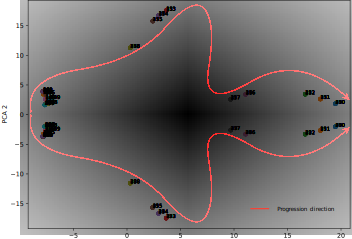
\includegraphics[width=0.7\linewidth]{figures/transition_pca.pdf}
        \vspace{-0.3cm}
        \caption*{{\scriptsize ACP des trajectoires de transition dans \textit{Overcooked-AI}}}
        \label{fig:overcooked_pca}
      \end{figure}

      \vspace{-0.5cm}

      \begin{figure}[h!]
        \centering
        \includegraphics[trim=0cm 0cm 0cm 1cm, clip, width=0.8\linewidth]{figures/results_noncyber_learning.pdf}
        \vspace{-0.3cm}
        \caption*{{\scriptsize Courbes d'apprentissage}}
        \label{fig:noncyber_learning_curves}
      \end{figure}

    \end{column}

  \end{columns}

\end{frame}


\begin{frame}{Etude de cas}{Infrastructure d'entreprise~\parencite{cage-challenge-announcement}}

  \vspace{-0cm}

  \begin{columns}[c]

    \hspace{-0.5cm}

    \begin{column}{0.5\textwidth}

      \textbf{Trois modèles organisationnels :}
      \begin{itemize}
        \item Attaquant / défenseur aléatoire
        \item Attaquant / défenseur manuel
        \item Attaquant / défenseur apprenant
      \end{itemize}


      \vspace{1cm}


      \begin{figure}

        \centering
        \includegraphics[width=0.8\linewidth]{figures/network_infra.png}
        \caption*{Topologie de l'infrastructure d'entreprise à petite échelle.}
      \end{figure}

    \end{column}

    \hspace{-0.5cm}

    \begin{column}{0.5\textwidth}
      \hspace{1cm}

      \begin{figure}

        \centering
        \includegraphics[trim=0.1cm 1.4cm 0.1cm 0.1cm, clip, width=0.8\linewidth]{figures/attack_defense_tree.jpg}
        \caption*{Arbre d'attaque/défense utilisé dans le scnéario CAGE Challenge n°1~\parencite{cage-challenge-announcement}. et \textbf{MITRE ATT\&CK} \parencite{MITREATTACKWebiste}.}

      \end{figure}

    \end{column}

  \end{columns}


\end{frame}

% \begin{frame}{Etude de cas}{Infrastructure d'entreprise}

%   \vspace{-0.5cm}

%   \begin{columns}[c]

%     \hspace{-0cm}

%     \begin{column}{0.5\textwidth}
%       {\scriptsize
%         \textbf{Principaux résultats :}
%         \begin{itemize}

%           \item Modélisation
%                 \begin{itemize}
%                   \item Validé quand dataset de trajectoires \textquote{assez important} (>5 Go)
%                 \end{itemize}

%           \item Entrainement
%                 \begin{itemize}
%                   \item Validé vis-à-vis du respect des contraintes dures et douces (taux de violation 0 pour dureté de contraintes forte)
%                 \end{itemize}

%           \item Analyse
%                 \begin{itemize}
%                   \item Validé rôles et objectifs inférées correspondent aux attentes (vérification manuelle des trajectoires produites)
%                 \end{itemize}

%           \item Transfert
%                 \begin{itemize}
%                   \item Validé prise en compte des modifications environnementales en temps réel (ajout/retrait d'un nœud dans le réseau)
%                 \end{itemize}

%         \end{itemize}
%       }
%     \end{column}

%     \begin{column}{0.5\textwidth}
%       \centering
%       \includegraphics[width=1\linewidth]{figures/company_infra_learning_curve.png}
%       \includegraphics[width=0.9\linewidth]{figures/infra_results.png}
%       \vspace{-1cm}
%     \end{column}

%   \end{columns}

% \end{frame}


\begin{frame}{Etude de cas}{Scénario essaim de drones~\parencite{cage_challenge_3_announcement}}

  \begin{columns}
    \begin{column}{0.5\textwidth}

      \textbf{Trois modèles d'organisation :}
      \begin{itemize}
        \item \textquote{Suspect Isolation}
        \item \textquote{Active Defense}
        \item \textquote{Manual}
      \end{itemize}

      \hspace{1.5cm}
      \makebox[0.4\textwidth][c]{\animategraphics[loop,autoplay,scale=0.19]{8}{figures/cyborg/frame}{0}{33}}

    \end{column}


    \begin{column}{0.5\textwidth}

      \vspace{-0.2cm}
      \centering

      \begin{figure}
        \centering
        \includegraphics[trim=0cm 2.4cm 0cm 0.2cm, clip,width=0.65\linewidth]{figures/markov_mdp_drones.png}
        \caption*{Diagramme de transition d'état pour un drone.}
      \end{figure}


      \vspace{-0.25cm}

      \begin{figure}
        \centering
        \includegraphics[trim=0cm 2cm 0cm 0cm, clip,width=0.6\linewidth]{figures/drones_illustration.png}
        \caption*{Scénario CAGE Challenge n°3~\parencite{cage_challenge_3_announcement} : protéger les drones \textquote{bons} des drones \textquote{infectés}.}
      \end{figure}

    \end{column}
  \end{columns}




\end{frame}

% \begin{frame}{Etude de cas}{Scénario essaim de drones}

%   \vspace{-0.5cm}

%   \begin{columns}[c]

%     \hspace{-0cm}

%     \begin{column}{0.5\textwidth}
%       {\scriptsize
%         \textbf{Principaux résultats :}
%         \begin{itemize}

%           \item Modélisation
%                 \begin{itemize}
%                   \item Validé quand dataset de trajectoires \textquote{assez important} (>5 Go)
%                 \end{itemize}

%           \item Entrainement
%                 \begin{itemize}
%                   \item Validé comme plus stable et plus grande convergence
%                 \end{itemize}

%           \item Analyse
%                 \begin{itemize}
%                   \item Validé rôles et objectifs inférées correspondent aux attentes (vérification manuelle des trajectoires produites)
%                 \end{itemize}

%           \item Transfert
%                 \begin{itemize}
%                   \item Validé prise en compte des modifications environnementales en temps réel (forcer un drone à être infecté pour déstabiliser)
%                 \end{itemize}

%         \end{itemize}
%       }
%     \end{column}

%     \begin{column}{0.5\textwidth}
%       \ \\ \ \\
%       \centering
%       \includegraphics[width=0.87\linewidth]{figures/drone_swarm_results.png}
%       \ \\ \ \medskip
%       \includegraphics[width=0.87\linewidth]{figures/cage_own_results.png}
%       \ \\ \ \medskip
%       \includegraphics[width=0.5\linewidth]{figures/cage_leader_results.png}
%     \end{column}

%   \end{columns}

% \end{frame}


\begin{frame}{Étude de cas}{Architecture des microservices Kubernetes}

  \centering
  % \includegraphics[width=0.7\linewidth]{figures/scenario_introduction.pdf}
  \resizebox{!}{0.8\textheight}{


\tikzset{every picture/.style={line width=0.75pt}} %set default line width to 0.75pt        

\begin{tikzpicture}[x=0.75pt,y=0.75pt,yscale=-1,xscale=1]
    %uncomment if require: \path (0,2246); %set diagram left start at 0, and has height of 2246

    %Shape: Smiley Face [id:dp4301091047275606] 
    \draw  [fill={rgb, 255:red, 74; green, 144; blue, 226 }  ,fill opacity=1 ][line width=1.5]  (190,1603.95) .. controls (190,1592.9) and (198.95,1583.95) .. (210,1583.95) .. controls (221.05,1583.95) and (230,1592.9) .. (230,1603.95) .. controls (230,1614.99) and (221.05,1623.95) .. (210,1623.95) .. controls (198.95,1623.95) and (190,1614.99) .. (190,1603.95) -- cycle ; \draw  [fill={rgb, 255:red, 74; green, 144; blue, 226 }  ,fill opacity=1 ][line width=1.5]  (201.2,1597.15) .. controls (201.2,1596.04) and (202.1,1595.15) .. (203.2,1595.15) .. controls (204.3,1595.15) and (205.2,1596.04) .. (205.2,1597.15) .. controls (205.2,1598.25) and (204.3,1599.15) .. (203.2,1599.15) .. controls (202.1,1599.15) and (201.2,1598.25) .. (201.2,1597.15) -- cycle ; \draw  [fill={rgb, 255:red, 74; green, 144; blue, 226 }  ,fill opacity=1 ][line width=1.5]  (214.8,1597.15) .. controls (214.8,1596.04) and (215.7,1595.15) .. (216.8,1595.15) .. controls (217.9,1595.15) and (218.8,1596.04) .. (218.8,1597.15) .. controls (218.8,1598.25) and (217.9,1599.15) .. (216.8,1599.15) .. controls (215.7,1599.15) and (214.8,1598.25) .. (214.8,1597.15) -- cycle ; \draw  [line width=1.5]  (200,1611.95) .. controls (206.67,1617.28) and (213.33,1617.28) .. (220,1611.95) ;
    %Shape: Circle [id:dp04794925319690546] 
    \draw  [fill={rgb, 255:red, 208; green, 2; blue, 27 }  ,fill opacity=1 ][line width=1.5]  (30,1388.95) .. controls (30,1377.9) and (38.95,1368.95) .. (50,1368.95) .. controls (61.05,1368.95) and (70,1377.9) .. (70,1388.95) .. controls (70,1399.99) and (61.05,1408.95) .. (50,1408.95) .. controls (38.95,1408.95) and (30,1399.99) .. (30,1388.95) -- cycle ;
    %Shape: Ellipse [id:dp1288230259059161] 
    \draw  [fill={rgb, 255:red, 208; green, 2; blue, 27 }  ,fill opacity=1 ][line width=1.5]  (40.25,1381.74) .. controls (40.25,1380.52) and (41.31,1379.53) .. (42.63,1379.53) .. controls (43.94,1379.53) and (45,1380.52) .. (45,1381.74) .. controls (45,1382.96) and (43.94,1383.95) .. (42.63,1383.95) .. controls (41.31,1383.95) and (40.25,1382.96) .. (40.25,1381.74) -- cycle ;
    %Shape: Ellipse [id:dp07141223501259764] 
    \draw  [fill={rgb, 255:red, 208; green, 2; blue, 27 }  ,fill opacity=1 ][line width=1.5]  (55.25,1381.74) .. controls (55.25,1380.52) and (56.31,1379.53) .. (57.63,1379.53) .. controls (58.94,1379.53) and (60,1380.52) .. (60,1381.74) .. controls (60,1382.96) and (58.94,1383.95) .. (57.63,1383.95) .. controls (56.31,1383.95) and (55.25,1382.96) .. (55.25,1381.74) -- cycle ;
    %Curve Lines [id:da4492744513284357] 
    \draw [fill={rgb, 255:red, 208; green, 2; blue, 27 }  ,fill opacity=1 ][line width=1.5]    (40,1398.95) .. controls (45.25,1393.93) and (55,1393.8) .. (60,1398.95) ;

    %Image [id:dp13678418305594697] 
    \draw (157.56,1371.71) node  {\includegraphics[width=18.66pt,height=18.36pt]{figures/pod.png}};
    %Shape: Rectangle [id:dp07803554532308699] 
    \draw  [color={rgb, 255:red, 74; green, 144; blue, 226 }  ,draw opacity=1 ][line width=1.5]  (135,1356.95) .. controls (135,1354.19) and (137.24,1351.95) .. (140,1351.95) -- (240,1351.95) .. controls (242.76,1351.95) and (245,1354.19) .. (245,1356.95) -- (245,1388.95) .. controls (245,1391.71) and (242.76,1393.95) .. (240,1393.95) -- (140,1393.95) .. controls (137.24,1393.95) and (135,1391.71) .. (135,1388.95) -- cycle ;
    %Image [id:dp09637293080723774] 
    \draw (222.5,1474.47) node  {\includegraphics[width=3.75pt,height=7.5pt]{figures/a5f8ecbd-6bf2-47fe-8fda-e2f613f70dd8.png}};
    %Image [id:dp19456179769a5f8ecbd-6bf2-47fe-8fda-e2f613f70dd8013326] 
    \draw (212.44,1486.71) node  {\includegraphics[width=18.66pt,height=18.36pt]{figures/pod.png}};

    %Image [id:dp5617243932186045] 
    \draw (585.71,1483.5) node  {\includegraphics[width=48.75pt,height=26.25pt]{figures/operational_resilience.png}};
    %Shape: Smiley Face [id:dp7881743196067302] 
    \draw  [fill={rgb, 255:red, 74; green, 144; blue, 226 }  ,fill opacity=1 ][line width=1.5]  (255,1603.95) .. controls (255,1592.9) and (263.95,1583.95) .. (275,1583.95) .. controls (286.05,1583.95) and (295,1592.9) .. (295,1603.95) .. controls (295,1614.99) and (286.05,1623.95) .. (275,1623.95) .. controls (263.95,1623.95) and (255,1614.99) .. (255,1603.95) -- cycle ; \draw  [fill={rgb, 255:red, 74; green, 144; blue, 226 }  ,fill opacity=1 ][line width=1.5]  (266.2,1597.15) .. controls (266.2,1596.04) and (267.1,1595.15) .. (268.2,1595.15) .. controls (269.3,1595.15) and (270.2,1596.04) .. (270.2,1597.15) .. controls (270.2,1598.25) and (269.3,1599.15) .. (268.2,1599.15) .. controls (267.1,1599.15) and (266.2,1598.25) .. (266.2,1597.15) -- cycle ; \draw  [fill={rgb, 255:red, 74; green, 144; blue, 226 }  ,fill opacity=1 ][line width=1.5]  (279.8,1597.15) .. controls (279.8,1596.04) and (280.7,1595.15) .. (281.8,1595.15) .. controls (282.9,1595.15) and (283.8,1596.04) .. (283.8,1597.15) .. controls (283.8,1598.25) and (282.9,1599.15) .. (281.8,1599.15) .. controls (280.7,1599.15) and (279.8,1598.25) .. (279.8,1597.15) -- cycle ; \draw  [line width=1.5]  (265,1611.95) .. controls (271.67,1617.28) and (278.33,1617.28) .. (285,1611.95) ;
    %Shape: Smiley Face [id:dp0022542805445343594] 
    \draw  [fill={rgb, 255:red, 74; green, 144; blue, 226 }  ,fill opacity=1 ][line width=1.5]  (320,1603.95) .. controls (320,1592.9) and (328.95,1583.95) .. (340,1583.95) .. controls (351.05,1583.95) and (360,1592.9) .. (360,1603.95) .. controls (360,1614.99) and (351.05,1623.95) .. (340,1623.95) .. controls (328.95,1623.95) and (320,1614.99) .. (320,1603.95) -- cycle ; \draw  [fill={rgb, 255:red, 74; green, 144; blue, 226 }  ,fill opacity=1 ][line width=1.5]  (331.2,1597.15) .. controls (331.2,1596.04) and (332.1,1595.15) .. (333.2,1595.15) .. controls (334.3,1595.15) and (335.2,1596.04) .. (335.2,1597.15) .. controls (335.2,1598.25) and (334.3,1599.15) .. (333.2,1599.15) .. controls (332.1,1599.15) and (331.2,1598.25) .. (331.2,1597.15) -- cycle ; \draw  [fill={rgb, 255:red, 74; green, 144; blue, 226 }  ,fill opacity=1 ][line width=1.5]  (344.8,1597.15) .. controls (344.8,1596.04) and (345.7,1595.15) .. (346.8,1595.15) .. controls (347.9,1595.15) and (348.8,1596.04) .. (348.8,1597.15) .. controls (348.8,1598.25) and (347.9,1599.15) .. (346.8,1599.15) .. controls (345.7,1599.15) and (344.8,1598.25) .. (344.8,1597.15) -- cycle ; \draw  [line width=1.5]  (330,1611.95) .. controls (336.67,1617.28) and (343.33,1617.28) .. (350,1611.95) ;
    %Shape: Smiley Face [id:dp10172496147554921] 
    \draw  [fill={rgb, 255:red, 74; green, 144; blue, 226 }  ,fill opacity=1 ][line width=1.5]  (385,1603.95) .. controls (385,1592.9) and (393.95,1583.95) .. (405,1583.95) .. controls (416.05,1583.95) and (425,1592.9) .. (425,1603.95) .. controls (425,1614.99) and (416.05,1623.95) .. (405,1623.95) .. controls (393.95,1623.95) and (385,1614.99) .. (385,1603.95) -- cycle ; \draw  [fill={rgb, 255:red, 74; green, 144; blue, 226 }  ,fill opacity=1 ][line width=1.5]  (396.2,1597.15) .. controls (396.2,1596.04) and (397.1,1595.15) .. (398.2,1595.15) .. controls (399.3,1595.15) and (400.2,1596.04) .. (400.2,1597.15) .. controls (400.2,1598.25) and (399.3,1599.15) .. (398.2,1599.15) .. controls (397.1,1599.15) and (396.2,1598.25) .. (396.2,1597.15) -- cycle ; \draw  [fill={rgb, 255:red, 74; green, 144; blue, 226 }  ,fill opacity=1 ][line width=1.5]  (409.8,1597.15) .. controls (409.8,1596.04) and (410.7,1595.15) .. (411.8,1595.15) .. controls (412.9,1595.15) and (413.8,1596.04) .. (413.8,1597.15) .. controls (413.8,1598.25) and (412.9,1599.15) .. (411.8,1599.15) .. controls (410.7,1599.15) and (409.8,1598.25) .. (409.8,1597.15) -- cycle ; \draw  [line width=1.5]  (395,1611.95) .. controls (401.67,1617.28) and (408.33,1617.28) .. (415,1611.95) ;
    %Image [id:dp875191805224898] 
    \draw (185.51,1346.45) node  {\includegraphics[width=18.75pt,height=18.75pt]{figures/service.jpg}};
    %Shape: Rectangle [id:dp16636202510740916] 
    \draw  [color={rgb, 255:red, 74; green, 144; blue, 226 }  ,draw opacity=1 ][line width=1.5]  (114.21,1308.95) .. controls (114.21,1306.18) and (116.45,1303.95) .. (119.21,1303.95) -- (480,1303.95) .. controls (482.76,1303.95) and (485,1306.18) .. (485,1308.95) -- (485,1520.94) .. controls (485,1523.7) and (482.76,1525.94) .. (480,1525.94) -- (119.21,1525.94) .. controls (116.45,1525.94) and (114.21,1523.7) .. (114.21,1520.94) -- cycle ;
    %Straight Lines [id:da6495577603694598] 
    \draw [color={rgb, 255:red, 245; green, 166; blue, 35 }  ,draw opacity=1 ][line width=5.25]    (485,1408.95) -- (531,1408.95) ;
    \draw [shift={(540,1408.95)}, rotate = 180] [fill={rgb, 255:red, 245; green, 166; blue, 35 }  ,fill opacity=1 ][line width=0.08]  [draw opacity=0] (16.61,-7.98) -- (0,0) -- (16.61,7.98) -- cycle    ;
    %Straight Lines [id:da8934771308658321] 
    \draw [color={rgb, 255:red, 208; green, 2; blue, 27 }  ,draw opacity=1 ][line width=6]    (74.83,1388.95) -- (104.21,1388.95) ;
    \draw [shift={(114.21,1388.95)}, rotate = 180] [fill={rgb, 255:red, 208; green, 2; blue, 27 }  ,fill opacity=1 ][line width=0.08]  [draw opacity=0] (19.82,-9.52) -- (0,0) -- (19.82,9.52) -- cycle    ;
    %Straight Lines [id:da4199022248159785] 
    \draw [color={rgb, 255:red, 126; green, 211; blue, 33 }  ,draw opacity=1 ][line width=6]    (74.83,1468.95) -- (104.21,1468.95) ;
    \draw [shift={(114.21,1468.95)}, rotate = 180] [fill={rgb, 255:red, 126; green, 211; blue, 33 }  ,fill opacity=1 ][line width=0.08]  [draw opacity=0] (19.82,-9.52) -- (0,0) -- (19.82,9.52) -- cycle    ;
    %Image [id:dp302283377689342] 
    \draw (47.5,1461.45) node  {\includegraphics[width=41.25pt,height=41.25pt]{figures/icons_521164.png}};
    %Image [id:dp7699140175350369] 
    \draw (157.56,1486.71) node  {\includegraphics[width=18.66pt,height=18.36pt]{figures/pod.png}};
    %Shape: Rectangle [id:dp9702984616712532] 
    \draw  [color={rgb, 255:red, 74; green, 144; blue, 226 }  ,draw opacity=1 ][line width=1.5]  (135,1471.95) .. controls (135,1469.19) and (137.24,1466.95) .. (140,1466.95) -- (240,1466.95) .. controls (242.76,1466.95) and (245,1469.19) .. (245,1471.95) -- (245,1503.95) .. controls (245,1506.71) and (242.76,1508.95) .. (240,1508.95) -- (140,1508.95) .. controls (137.24,1508.95) and (135,1506.71) .. (135,1503.95) -- cycle ;
    %Image [id:dp3271892586469496] 
    \draw (185.51,1461.45) node  {\includegraphics[width=18.75pt,height=18.75pt]{figures/service.jpg}};
    %Shape: Rectangle [id:dp24658484222832167] 
    \draw  [color={rgb, 255:red, 74; green, 144; blue, 226 }  ,draw opacity=1 ][line width=1.5]  (240,1421.95) .. controls (240,1419.19) and (242.24,1416.95) .. (245,1416.95) -- (345,1416.95) .. controls (347.76,1416.95) and (350,1419.19) .. (350,1421.95) -- (350,1453.95) .. controls (350,1456.71) and (347.76,1458.95) .. (345,1458.95) -- (245,1458.95) .. controls (242.24,1458.95) and (240,1456.71) .. (240,1453.95) -- cycle ;
    %Image [id:dp8244306742841939] 
    \draw (290.51,1411.45) node  {\includegraphics[width=18.75pt,height=18.75pt]{figures/service.jpg}};
    %Image [id:dp4194584522849387] 
    \draw (426.61,1370.69) node  {\includegraphics[width=17.42pt,height=17.62pt]{figures/a5f8ecbd-6bf2-47fe-8fda-e2f613f70dd8.png}};
    %Shape: Rectangle [id:dp9521856660402277] 
    \draw  [color={rgb, 255:red, 74; green, 144; blue, 226 }  ,draw opacity=1 ][line width=1.5]  (345,1356.95) .. controls (345,1354.19) and (347.24,1351.95) .. (350,1351.95) -- (450,1351.95) .. controls (452.76,1351.95) and (455,1354.19) .. (455,1356.95) -- (455,1388.95) .. controls (455,1391.71) and (452.76,1393.95) .. (450,1393.95) -- (350,1393.95) .. controls (347.24,1393.95) and (345,1391.71) .. (345,1388.95) -- cycle ;
    %Image [id:dp17468043606691175] 
    \draw (395.51,1346.45) node  {\includegraphics[width=18.75pt,height=18.75pt]{figures/service.jpg}};
    %Image [id:dp6985629115383786] 
    \draw (367.56,1491.71) node  {\includegraphics[width=18.66pt,height=18.36pt]{figures/pod.png}};
    %Shape: Rectangle [id:dp3224466801208138] 
    \draw  [color={rgb, 255:red, 74; green, 144; blue, 226 }  ,draw opacity=1 ][line width=1.5]  (345,1476.95) .. controls (345,1474.19) and (347.24,1471.95) .. (350,1471.95) -- (450,1471.95) .. controls (452.76,1471.95) and (455,1474.19) .. (455,1476.95) -- (455,1508.95) .. controls (455,1511.71) and (452.76,1513.95) .. (450,1513.95) -- (350,1513.95) .. controls (347.24,1513.95) and (345,1511.71) .. (345,1508.95) -- cycle ;
    %Image [id:dp47078330482310293] 
    \draw (395.51,1466.45) node  {\includegraphics[width=18.75pt,height=18.75pt]{figures/service.jpg}};
    %Image [id:dp49328474155004964] 
    \draw (290.62,1295.03) node  {\includegraphics[width=38.42pt,height=37.55pt]{figures/kubernetes_cluster.png}};
    %Image [id:dp07503368448805825] 
    \draw (367.44,1371.71) node  {\includegraphics[width=18.66pt,height=18.36pt]{figures/pod.png}};
    %Image [id:dp4607494985107903] 
    \draw (377.5,1358.95) node  {\includegraphics[width=11.25pt,height=7.5pt]{figures/contention-removebg-preview.png}};

    %Image [id:dp5420016495908997] 
    \draw (212.44,1371.71) node  {\includegraphics[width=18.66pt,height=18.36pt]{figures/pod.png}};
    %Image [id:dp11441370230026127] 
    \draw (437.5,1479.47) node  {\includegraphics[width=3.75pt,height=7.5pt]{figures/a5f8ecbd-6bf2-47fe-8fda-e2f613f70dd8.png}};
    %Image [id:dp41191486143412925] 
    \draw (427.44,1491.71) node  {\includegraphics[width=18.66pt,height=18.36pt]{figures/pod.png}};
    %Image [id:dp714626695045933] 
    \draw (367.5,1613.95) node  {\includegraphics[width=3.75pt,height=7.5pt]{figures/a5f8ecbd-6bf2-47fe-8fda-e2f613f70dd8.png}};
    %Image [id:dp017291826703530244] 
    \draw (357.44,1626.18) node  {\includegraphics[width=18.66pt,height=18.36pt]{figures/pod.png}};
    %Image [id:dp13073525089863725] 
    \draw (422.44,1626.71) node  {\includegraphics[width=18.66pt,height=18.36pt]{figures/pod.png}};
    %Image [id:dp9012746994003437] 
    \draw (432.5,1613.95) node  {\includegraphics[width=11.25pt,height=7.5pt]{figures/contention-removebg-preview.png}};
    %Straight Lines [id:da8457135870612951] 
    \draw [color={rgb, 255:red, 126; green, 211; blue, 33 }  ,draw opacity=1 ][line width=3]    (245,1488.95) -- (299.63,1461.63) ;
    \draw [shift={(305,1458.95)}, rotate = 153.43] [fill={rgb, 255:red, 126; green, 211; blue, 33 }  ,fill opacity=1 ][line width=0.08]  [draw opacity=0] (10.18,-4.89) -- (0,0) -- (10.18,4.89) -- cycle    ;
    %Straight Lines [id:da380207509604092] 
    \draw [color={rgb, 255:red, 126; green, 211; blue, 33 }  ,draw opacity=1 ][line width=3]    (305,1458.95) -- (340.48,1489.99) ;
    \draw [shift={(345,1493.95)}, rotate = 221.19] [fill={rgb, 255:red, 126; green, 211; blue, 33 }  ,fill opacity=1 ][line width=0.08]  [draw opacity=0] (10.18,-4.89) -- (0,0) -- (10.18,4.89) -- cycle    ;
    %Image [id:dp4293736210756913] 
    \draw (262.44,1436.71) node  {\includegraphics[width=18.66pt,height=18.36pt]{figures/pod.png}};
    %Image [id:dp9307320072632751] 
    \draw (272.5,1423.95) node  {\includegraphics[width=11.25pt,height=7.5pt]{figures/contention-removebg-preview.png}};

    %Straight Lines [id:da8183896833003403] 
    \draw [color={rgb, 255:red, 126; green, 211; blue, 33 }  ,draw opacity=1 ][line width=3]    (350,1443.95) -- (400.56,1397.98) ;
    \draw [shift={(405,1393.95)}, rotate = 137.73] [fill={rgb, 255:red, 126; green, 211; blue, 33 }  ,fill opacity=1 ][line width=0.08]  [draw opacity=0] (10.18,-4.89) -- (0,0) -- (10.18,4.89) -- cycle    ;
    %Straight Lines [id:da9515263644688517] 
    \draw [color={rgb, 255:red, 126; green, 211; blue, 33 }  ,draw opacity=1 ][line width=3]    (114.21,1468.95) -- (176.04,1398.46) ;
    \draw [shift={(180,1393.95)}, rotate = 131.26] [fill={rgb, 255:red, 126; green, 211; blue, 33 }  ,fill opacity=1 ][line width=0.08]  [draw opacity=0] (10.18,-4.89) -- (0,0) -- (10.18,4.89) -- cycle    ;
    %Straight Lines [id:da5503931860153507] 
    \draw [color={rgb, 255:red, 126; green, 211; blue, 33 }  ,draw opacity=1 ][line width=3]    (115,1468.95) -- (131.25,1489.26) ;
    \draw [shift={(135,1493.95)}, rotate = 231.34] [fill={rgb, 255:red, 126; green, 211; blue, 33 }  ,fill opacity=1 ][line width=0.08]  [draw opacity=0] (10.18,-4.89) -- (0,0) -- (10.18,4.89) -- cycle    ;
    %Straight Lines [id:da6047412034272691] 
    \draw [color={rgb, 255:red, 208; green, 2; blue, 27 }  ,draw opacity=1 ][line width=3]    (114.21,1388.95) -- (130.13,1377.46) ;
    \draw [shift={(135,1373.95)}, rotate = 144.19] [fill={rgb, 255:red, 208; green, 2; blue, 27 }  ,fill opacity=1 ][line width=0.08]  [draw opacity=0] (10.18,-4.89) -- (0,0) -- (10.18,4.89) -- cycle    ;
    %Straight Lines [id:da23596431797867] 
    \draw [color={rgb, 255:red, 208; green, 2; blue, 27 }  ,draw opacity=1 ][line width=3]    (114.21,1388.95) -- (152.27,1463.6) ;
    \draw [shift={(155,1468.95)}, rotate = 242.98] [fill={rgb, 255:red, 208; green, 2; blue, 27 }  ,fill opacity=1 ][line width=0.08]  [draw opacity=0] (10.18,-4.89) -- (0,0) -- (10.18,4.89) -- cycle    ;
    %Straight Lines [id:da05747957902862033] 
    \draw [color={rgb, 255:red, 208; green, 2; blue, 27 }  ,draw opacity=1 ][line width=3]    (245,1373.95) -- (339,1373.95) ;
    \draw [shift={(345,1373.95)}, rotate = 180] [fill={rgb, 255:red, 208; green, 2; blue, 27 }  ,fill opacity=1 ][line width=0.08]  [draw opacity=0] (10.18,-4.89) -- (0,0) -- (10.18,4.89) -- cycle    ;
    %Straight Lines [id:da5601728845971867] 
    \draw [color={rgb, 255:red, 126; green, 211; blue, 33 }  ,draw opacity=1 ][line width=3]    (455,1373.95) -- (481.1,1404.39) ;
    \draw [shift={(485,1408.95)}, rotate = 229.4] [fill={rgb, 255:red, 126; green, 211; blue, 33 }  ,fill opacity=1 ][line width=0.08]  [draw opacity=0] (10.18,-4.89) -- (0,0) -- (10.18,4.89) -- cycle    ;
    %Straight Lines [id:da418872346597604] 
    \draw [color={rgb, 255:red, 126; green, 211; blue, 33 }  ,draw opacity=1 ][line width=3]    (455,1493.95) -- (483,1414.6) ;
    \draw [shift={(485,1408.95)}, rotate = 109.44] [fill={rgb, 255:red, 126; green, 211; blue, 33 }  ,fill opacity=1 ][line width=0.08]  [draw opacity=0] (10.18,-4.89) -- (0,0) -- (10.18,4.89) -- cycle    ;
    %Straight Lines [id:da5389403615477466] 
    \draw [color={rgb, 255:red, 208; green, 2; blue, 27 }  ,draw opacity=1 ][line width=3]    (405,1393.95) -- (442.18,1463.65) ;
    \draw [shift={(445,1468.95)}, rotate = 241.93] [fill={rgb, 255:red, 208; green, 2; blue, 27 }  ,fill opacity=1 ][line width=0.08]  [draw opacity=0] (10.18,-4.89) -- (0,0) -- (10.18,4.89) -- cycle    ;
    %Straight Lines [id:da0689060436231772] 
    \draw [color={rgb, 255:red, 74; green, 144; blue, 226 }  ,draw opacity=1 ][line width=5.25]    (209.88,1569.95) -- (209.97,1537.95) ;
    \draw [shift={(210,1528.95)}, rotate = 90.17] [fill={rgb, 255:red, 74; green, 144; blue, 226 }  ,fill opacity=1 ][line width=0.08]  [draw opacity=0] (16.61,-7.98) -- (0,0) -- (16.61,7.98) -- cycle    ;
    \draw [shift={(209.86,1578.95)}, rotate = 270.17] [fill={rgb, 255:red, 74; green, 144; blue, 226 }  ,fill opacity=1 ][line width=0.08]  [draw opacity=0] (16.61,-7.98) -- (0,0) -- (16.61,7.98) -- cycle    ;
    %Straight Lines [id:da4654056477665215] 
    \draw [color={rgb, 255:red, 74; green, 144; blue, 226 }  ,draw opacity=1 ][line width=5.25]    (404.88,1569.95) -- (404.97,1537.95) ;
    \draw [shift={(405,1528.95)}, rotate = 90.17] [fill={rgb, 255:red, 74; green, 144; blue, 226 }  ,fill opacity=1 ][line width=0.08]  [draw opacity=0] (16.61,-7.98) -- (0,0) -- (16.61,7.98) -- cycle    ;
    \draw [shift={(404.86,1578.95)}, rotate = 270.17] [fill={rgb, 255:red, 74; green, 144; blue, 226 }  ,fill opacity=1 ][line width=0.08]  [draw opacity=0] (16.61,-7.98) -- (0,0) -- (16.61,7.98) -- cycle    ;
    %Straight Lines [id:da5630946115739178] 
    \draw [color={rgb, 255:red, 74; green, 144; blue, 226 }  ,draw opacity=1 ][line width=5.25]    (274.88,1569.95) -- (274.97,1537.95) ;
    \draw [shift={(275,1528.95)}, rotate = 90.17] [fill={rgb, 255:red, 74; green, 144; blue, 226 }  ,fill opacity=1 ][line width=0.08]  [draw opacity=0] (16.61,-7.98) -- (0,0) -- (16.61,7.98) -- cycle    ;
    \draw [shift={(274.86,1578.95)}, rotate = 270.17] [fill={rgb, 255:red, 74; green, 144; blue, 226 }  ,fill opacity=1 ][line width=0.08]  [draw opacity=0] (16.61,-7.98) -- (0,0) -- (16.61,7.98) -- cycle    ;
    %Straight Lines [id:da9201077281295033] 
    \draw [color={rgb, 255:red, 74; green, 144; blue, 226 }  ,draw opacity=1 ][line width=5.25]    (339.88,1569.95) -- (339.97,1537.95) ;
    \draw [shift={(340,1528.95)}, rotate = 90.17] [fill={rgb, 255:red, 74; green, 144; blue, 226 }  ,fill opacity=1 ][line width=0.08]  [draw opacity=0] (16.61,-7.98) -- (0,0) -- (16.61,7.98) -- cycle    ;
    \draw [shift={(339.86,1578.95)}, rotate = 270.17] [fill={rgb, 255:red, 74; green, 144; blue, 226 }  ,fill opacity=1 ][line width=0.08]  [draw opacity=0] (16.61,-7.98) -- (0,0) -- (16.61,7.98) -- cycle    ;
    %Image [id:dp037278758736594586] 
    \draw (332.5,1423.95) node  {\includegraphics[width=11.25pt,height=7.5pt]{figures/bottleneck.png}};
    %Image [id:dp9635867942890575] 
    \draw (317.44,1436.71) node  {\includegraphics[width=18.66pt,height=18.36pt]{figures/pod.png}};

    %Straight Lines [id:da4979664991834727] 
    \draw [color={rgb, 255:red, 208; green, 2; blue, 27 }  ,draw opacity=1 ][line width=3]    (245,1373.95) -- (257.89,1408.33) ;
    \draw [shift={(260,1413.95)}, rotate = 249.44] [fill={rgb, 255:red, 208; green, 2; blue, 27 }  ,fill opacity=1 ][line width=0.08]  [draw opacity=0] (10.18,-4.89) -- (0,0) -- (10.18,4.89) -- cycle    ;
    %Image [id:dp5896117385768661] 
    \draw (352.5,1443.95) node  {\includegraphics[width=11.25pt,height=7.5pt]{figures/bottleneck.png}};
    %Image [id:dp7535006751613231] 
    \draw (302.5,1613.95) node  {\includegraphics[width=11.25pt,height=7.5pt]{figures/bottleneck.png}};
    %Image [id:dp3671930350021573] 
    \draw (287.44,1626.71) node  {\includegraphics[width=18.66pt,height=18.36pt]{figures/pod.png}};
    %Image [id:dp30057123810502306] 
    \draw (227.5,1626.45) node  {\includegraphics[width=18.75pt,height=18.75pt]{figures/a5f8ecbd-6bf2-47fe-8fda-e2f613f70dd8-removebg-preview.png}};
    %Straight Lines [id:da9635361631974899] 
    \draw [color={rgb, 255:red, 74; green, 144; blue, 226 }  ,draw opacity=1 ][line width=5.25]    (464,1603.95) -- (585,1603.95) -- (585,1547.95) ;
    \draw [shift={(585,1538.95)}, rotate = 90] [fill={rgb, 255:red, 74; green, 144; blue, 226 }  ,fill opacity=1 ][line width=0.08]  [draw opacity=0] (16.61,-7.98) -- (0,0) -- (16.61,7.98) -- cycle    ;
    \draw [shift={(455,1603.95)}, rotate = 0] [fill={rgb, 255:red, 74; green, 144; blue, 226 }  ,fill opacity=1 ][line width=0.08]  [draw opacity=0] (16.61,-7.98) -- (0,0) -- (16.61,7.98) -- cycle    ;


    % Text Node
    \draw (345,1654.5) node  [font=\small] [align=left] {DDoS};
    % Text Node
    \draw (420,1654.5) node  [font=\small] [align=left] {accaparement};
    % Text Node
    \draw (278.5,1654.5) node  [font=\small] [align=left] {goulot étr.};
    % Text Node
    \draw (208.5,1654.5) node  [font=\small] [align=left] {crash};
    % Text Node
    \draw (146,1603.45) node  [font=\small] [align=left] {défenseurs};
    % Text Node
    \draw (51,1353.45) node  [font=\small] [align=left] {attaquant};
    % Text Node
    \draw (396.5,1443.45) node  [font=\small] [align=left] {service};
    % Text Node
    \draw (392.5,1489.95) node  [font=\tiny] [align=left] {{\LARGE {\fontfamily{helvet}\selectfont \textcolor[rgb]{0.29,0.56,0.89}{...}}}};
    % Text Node
    \draw (396.5,1323.45) node  [font=\small] [align=left] {service};
    % Text Node
    \draw (392.5,1369.95) node  [font=\tiny] [align=left] {{\LARGE {\fontfamily{helvet}\selectfont \textcolor[rgb]{0.29,0.56,0.89}{...}}}};
    % Text Node
    \draw (291.5,1388.45) node  [font=\small] [align=left] {service};
    % Text Node
    \draw (287.5,1434.95) node  [font=\tiny] [align=left] {{\LARGE {\fontfamily{helvet}\selectfont \textcolor[rgb]{0.29,0.56,0.89}{...}}}};
    % Text Node
    \draw (186.5,1438.45) node  [font=\small] [align=left] {service};
    % Text Node
    \draw (182.5,1484.95) node  [font=\tiny] [align=left] {{\LARGE {\fontfamily{helvet}\selectfont \textcolor[rgb]{0.29,0.56,0.89}{...}}}};
    % Text Node
    \draw (90.71,1489.45) node  [font=\small] [align=left] {input};
    % Text Node
    \draw (288.11,1329.45) node  [font=\small] [align=left] {cluster};
    % Text Node
    \draw (579,1514.45) node  [font=\small] [align=left] {résilience opérationnelle};
    % Text Node
    \draw (90.71,1409.45) node  [font=\small] [align=left] {input};
    % Text Node
    \draw (124,1550.5) node  [font=\small] [align=left] {\textit{actions mise à l'échelle}};
    % Text Node
    \draw (519,1428.45) node  [font=\small] [align=left] {output};
    % Text Node
    \draw (186.5,1323.45) node  [font=\small] [align=left] {service};
    % Text Node
    \draw (182.5,1369.95) node  [font=\tiny] [align=left] {{\LARGE {\fontfamily{helvet}\selectfont \textcolor[rgb]{0.29,0.56,0.89}{...}}}};


\end{tikzpicture}}

  \vfill

  {\tiny \begin{spacing}{0.8}
      \textit{J. Soule, J.-P. Jamont, M. Occello, L.-M. Traonouez, and P. Théron. Streamlining Resilient Kubernetes Autoscaling with Multi-Agent Systems via an Automated Online Design Framework. Proceedings of the 18th IEEE International Conference on Cloud Computing (CLOUD), Helsinki, Finland, July 2025.}
    \end{spacing}}

\end{frame}

\begin{frame}{Étude de cas}{Architecture des microservices Kubernetes}


  \begin{columns}[c]

    \begin{column}{0.4\textwidth}

      \textbf{Approche SMA}
      \begin{itemize}
        \item Un agent par problème
        \item Cibler les problèmes par priorité
        \item Changement d'échelle facilité
      \end{itemize}

      \

      \textbf{Mise en œuvre dans KARMA (\textit{Kubernetes Autoscaling with Resilient Multi-Agent system})}
      \begin{itemize}
        \item PoC fonctionnel sur cluster simple
        \item Amélioration résilience opérationnelle
        \item Convergence plus rapide
      \end{itemize}

    \end{column}

    \begin{column}{0.7\textwidth}

      \resizebox{1\linewidth}{!}{


\tikzset{every picture/.style={line width=0.75pt}} %set default line width to 0.75pt        

\begin{tikzpicture}[x=0.75pt,y=0.75pt,yscale=-1.2,xscale=1.2]
%uncomment if require: \path (0,1414); %set diagram left start at 0, and has height of 1414

%Straight Lines [id:da5609883377896374] 
\draw [color={rgb, 255:red, 74; green, 144; blue, 226 }  ,draw opacity=1 ][line width=2.25]    (317.22,111.13) -- (360.07,111.13) ;
\draw [shift={(365.07,111.13)}, rotate = 180] [fill={rgb, 255:red, 74; green, 144; blue, 226 }  ,fill opacity=1 ][line width=0.08]  [draw opacity=0] (5.72,-2.75) -- (0,0) -- (5.72,2.75) -- cycle    ;
%Image [id:dp9396292457736715] 
\draw (106.77,60.95) node  {\includegraphics[width=18.66pt,height=18.36pt]{figures/karma_architecture/pod.png}};
%Image [id:dp3874378335758297] 
\draw (145.86,60.95) node  {\includegraphics[width=18.66pt,height=18.36pt]{figures/karma_architecture/pod.png}};
%Shape: Rectangle [id:dp4562827234223257] 
\draw  [color={rgb, 255:red, 74; green, 144; blue, 226 }  ,draw opacity=1 ][line width=1.5]  (89,28.36) .. controls (89,25.6) and (91.24,23.36) .. (94,23.36) -- (255,23.36) .. controls (257.76,23.36) and (260,25.6) .. (260,28.36) -- (260,132) .. controls (260,134.76) and (257.76,137) .. (255,137) -- (94,137) .. controls (91.24,137) and (89,134.76) .. (89,132) -- cycle ;
%Image [id:dp9455935833751838] 
\draw (172.5,16.24) node  {\includegraphics[width=18.66pt,height=18.36pt]{figures/karma_architecture/kubernetes.png}};
%Shape: Rectangle [id:dp9564725691593288] 
\draw  [color={rgb, 255:red, 74; green, 144; blue, 226 }  ,draw opacity=1 ][line width=1.5]  (92.55,50.21) .. controls (92.55,47.45) and (94.79,45.21) .. (97.55,45.21) -- (155.08,45.21) .. controls (157.84,45.21) and (160.08,47.45) .. (160.08,50.21) -- (160.08,70.81) .. controls (160.08,73.57) and (157.84,75.81) .. (155.08,75.81) -- (97.55,75.81) .. controls (94.79,75.81) and (92.55,73.57) .. (92.55,70.81) -- cycle ;
%Image [id:dp9120856447688912] 
\draw (126.32,39.97) node  {\includegraphics[width=18.66pt,height=18.36pt]{figures/karma_architecture/node.png}};
%Image [id:dp5738167237736518] 
\draw (106.77,119.52) node  {\includegraphics[width=18.66pt,height=18.36pt]{figures/karma_architecture/pod.png}};
%Image [id:dp2199681121060142] 
\draw (145.86,119.52) node  {\includegraphics[width=18.66pt,height=18.36pt]{figures/karma_architecture/pod.png}};
%Shape: Rectangle [id:dp12159705904547402] 
\draw  [color={rgb, 255:red, 74; green, 144; blue, 226 }  ,draw opacity=1 ][line width=1.5]  (92.55,108.78) .. controls (92.55,106.02) and (94.79,103.78) .. (97.55,103.78) -- (155.08,103.78) .. controls (157.84,103.78) and (160.08,106.02) .. (160.08,108.78) -- (160.08,129.38) .. controls (160.08,132.14) and (157.84,134.38) .. (155.08,134.38) -- (97.55,134.38) .. controls (94.79,134.38) and (92.55,132.14) .. (92.55,129.38) -- cycle ;
%Image [id:dp37768653229718074] 
\draw (126.32,98.54) node  {\includegraphics[width=18.66pt,height=18.36pt]{figures/karma_architecture/node.png}};
%Shape: Rectangle [id:dp20840815212238661] 
\draw  [color={rgb, 255:red, 74; green, 144; blue, 226 }  ,draw opacity=1 ][line width=1.5]  (264,28.36) .. controls (264,25.6) and (266.24,23.36) .. (269,23.36) -- (411.78,23.36) .. controls (414.54,23.36) and (416.78,25.6) .. (416.78,28.36) -- (416.78,132) .. controls (416.78,134.76) and (414.54,137) .. (411.78,137) -- (269,137) .. controls (266.24,137) and (264,134.76) .. (264,132) -- cycle ;
%Straight Lines [id:da9232180983272227] 
\draw [color={rgb, 255:red, 74; green, 144; blue, 226 }  ,draw opacity=1 ][line width=2.25]    (164,112) -- (201,112) ;
\draw [shift={(206,112)}, rotate = 180] [fill={rgb, 255:red, 74; green, 144; blue, 226 }  ,fill opacity=1 ][line width=0.08]  [draw opacity=0] (5.72,-2.75) -- (0,0) -- (5.72,2.75) -- cycle    ;
%Straight Lines [id:da6082715106712999] 
\draw [color={rgb, 255:red, 74; green, 144; blue, 226 }  ,draw opacity=1 ][line width=2.25]    (180,90.22) -- (167,90.22) ;
\draw [shift={(162,90.22)}, rotate = 360] [fill={rgb, 255:red, 74; green, 144; blue, 226 }  ,fill opacity=1 ][line width=0.08]  [draw opacity=0] (5.72,-2.75) -- (0,0) -- (5.72,2.75) -- cycle    ;
%Straight Lines [id:da30764510910060716] 
\draw [color={rgb, 255:red, 74; green, 144; blue, 226 }  ,draw opacity=1 ][line width=2.25]    (210,72) -- (199,72) ;
\draw [shift={(194,72)}, rotate = 360] [fill={rgb, 255:red, 74; green, 144; blue, 226 }  ,fill opacity=1 ][line width=0.08]  [draw opacity=0] (5.72,-2.75) -- (0,0) -- (5.72,2.75) -- cycle    ;
%Straight Lines [id:da5394403186779959] 
\draw [color={rgb, 255:red, 74; green, 144; blue, 226 }  ,draw opacity=1 ][line width=2.25]    (178,56.22) -- (167,56.22) ;
\draw [shift={(162,56.22)}, rotate = 360] [fill={rgb, 255:red, 74; green, 144; blue, 226 }  ,fill opacity=1 ][line width=0.08]  [draw opacity=0] (5.72,-2.75) -- (0,0) -- (5.72,2.75) -- cycle    ;
%Straight Lines [id:da6399475815904785] 
\draw [color={rgb, 255:red, 74; green, 144; blue, 226 }  ,draw opacity=1 ][line width=2.25]    (272,72) -- (235,72) ;
\draw [shift={(230,72)}, rotate = 360] [fill={rgb, 255:red, 74; green, 144; blue, 226 }  ,fill opacity=1 ][line width=0.08]  [draw opacity=0] (5.72,-2.75) -- (0,0) -- (5.72,2.75) -- cycle    ;
%Straight Lines [id:da24320102833940327] 
\draw [color={rgb, 255:red, 74; green, 144; blue, 226 }  ,draw opacity=1 ][line width=2.25]    (267,112) -- (230,112) ;
\draw [shift={(272,112)}, rotate = 180] [fill={rgb, 255:red, 74; green, 144; blue, 226 }  ,fill opacity=1 ][line width=0.08]  [draw opacity=0] (5.72,-2.75) -- (0,0) -- (5.72,2.75) -- cycle    ;
%Shape: Rectangle [id:dp9149123987409296] 
\draw  [color={rgb, 255:red, 255; green, 255; blue, 255 }  ,draw opacity=1 ][fill={rgb, 255:red, 255; green, 255; blue, 255 }  ,fill opacity=1 ] (328.83,106.67) -- (353.11,106.67) -- (353.11,114) -- (328.83,114) -- cycle ;
%Image [id:dp7127891043436136] 
\draw (341.68,109.47) node  {\includegraphics[width=14.57pt,height=15.21pt]{figures/karma_architecture/pettingzoo.png}};
%Straight Lines [id:da5757027637146572] 
\draw [color={rgb, 255:red, 74; green, 144; blue, 226 }  ,draw opacity=1 ][line width=2.25]    (357.9,41) -- (364.9,41) ;
\draw [shift={(352.9,41)}, rotate = 0] [fill={rgb, 255:red, 74; green, 144; blue, 226 }  ,fill opacity=1 ][line width=0.08]  [draw opacity=0] (5.72,-2.75) -- (0,0) -- (5.72,2.75) -- cycle    ;
%Straight Lines [id:da29364722138505184] 
\draw [color={rgb, 255:red, 74; green, 144; blue, 226 }  ,draw opacity=1 ][line width=2.25]    (390.99,97.77) -- (390.99,57.25) ;
\draw [shift={(390.99,52.25)}, rotate = 90] [fill={rgb, 255:red, 74; green, 144; blue, 226 }  ,fill opacity=1 ][line width=0.08]  [draw opacity=0] (5.72,-2.75) -- (0,0) -- (5.72,2.75) -- cycle    ;
%Straight Lines [id:da5470457469462804] 
\draw [color={rgb, 255:red, 74; green, 144; blue, 226 }  ,draw opacity=1 ][line width=2.25]    (390.9,71) -- (325.9,71) ;
\draw [shift={(320.9,71)}, rotate = 360] [fill={rgb, 255:red, 74; green, 144; blue, 226 }  ,fill opacity=1 ][line width=0.08]  [draw opacity=0] (5.72,-2.75) -- (0,0) -- (5.72,2.75) -- cycle    ;
%Shape: Rectangle [id:dp8476965567779329] 
\draw  [color={rgb, 255:red, 255; green, 255; blue, 255 }  ,draw opacity=1 ][fill={rgb, 255:red, 255; green, 255; blue, 255 }  ,fill opacity=1 ] (378.41,65.11) -- (397.83,65.11) -- (397.83,92) -- (378.41,92) -- cycle ;
%Shape: Smiley Face [id:dp8656850497140396] 
\draw  [fill={rgb, 255:red, 255; green, 255; blue, 255 }  ,fill opacity=1 ][line width=0.75]  (380.35,69.4) .. controls (380.35,67.3) and (382.09,65.6) .. (384.24,65.6) .. controls (386.38,65.6) and (388.12,67.3) .. (388.12,69.4) .. controls (388.12,71.5) and (386.38,73.2) .. (384.24,73.2) .. controls (382.09,73.2) and (380.35,71.5) .. (380.35,69.4) -- cycle ; \draw  [fill={rgb, 255:red, 255; green, 255; blue, 255 }  ,fill opacity=1 ][line width=0.75]  (382.53,68.11) .. controls (382.53,67.9) and (382.7,67.73) .. (382.92,67.73) .. controls (383.13,67.73) and (383.31,67.9) .. (383.31,68.11) .. controls (383.31,68.32) and (383.13,68.49) .. (382.92,68.49) .. controls (382.7,68.49) and (382.53,68.32) .. (382.53,68.11) -- cycle ; \draw  [fill={rgb, 255:red, 255; green, 255; blue, 255 }  ,fill opacity=1 ][line width=0.75]  (385.17,68.11) .. controls (385.17,67.9) and (385.34,67.73) .. (385.56,67.73) .. controls (385.77,67.73) and (385.95,67.9) .. (385.95,68.11) .. controls (385.95,68.32) and (385.77,68.49) .. (385.56,68.49) .. controls (385.34,68.49) and (385.17,68.32) .. (385.17,68.11) -- cycle ; \draw  [line width=0.75]  (382.29,70.92) .. controls (383.59,71.94) and (384.88,71.94) .. (386.18,70.92) ;
%Shape: Smiley Face [id:dp9163740789669144] 
\draw  [fill={rgb, 255:red, 255; green, 255; blue, 255 }  ,fill opacity=1 ][line width=0.75]  (392.01,69.4) .. controls (392.01,67.3) and (393.75,65.6) .. (395.89,65.6) .. controls (398.04,65.6) and (399.78,67.3) .. (399.78,69.4) .. controls (399.78,71.5) and (398.04,73.2) .. (395.89,73.2) .. controls (393.75,73.2) and (392.01,71.5) .. (392.01,69.4) -- cycle ; \draw  [fill={rgb, 255:red, 255; green, 255; blue, 255 }  ,fill opacity=1 ][line width=0.75]  (394.18,68.11) .. controls (394.18,67.9) and (394.36,67.73) .. (394.57,67.73) .. controls (394.79,67.73) and (394.96,67.9) .. (394.96,68.11) .. controls (394.96,68.32) and (394.79,68.49) .. (394.57,68.49) .. controls (394.36,68.49) and (394.18,68.32) .. (394.18,68.11) -- cycle ; \draw  [fill={rgb, 255:red, 255; green, 255; blue, 255 }  ,fill opacity=1 ][line width=0.75]  (396.82,68.11) .. controls (396.82,67.9) and (397,67.73) .. (397.21,67.73) .. controls (397.43,67.73) and (397.6,67.9) .. (397.6,68.11) .. controls (397.6,68.32) and (397.43,68.49) .. (397.21,68.49) .. controls (397,68.49) and (396.82,68.32) .. (396.82,68.11) -- cycle ; \draw  [line width=0.75]  (393.95,70.92) .. controls (395.24,71.94) and (396.54,71.94) .. (397.83,70.92) ;
%Shape: Smiley Face [id:dp8186451078369623] 
\draw  [fill={rgb, 255:red, 255; green, 255; blue, 255 }  ,fill opacity=1 ][line width=0.75]  (386.18,77.44) .. controls (386.18,75.34) and (387.92,73.64) .. (390.06,73.64) .. controls (392.21,73.64) and (393.95,75.34) .. (393.95,77.44) .. controls (393.95,79.54) and (392.21,81.24) .. (390.06,81.24) .. controls (387.92,81.24) and (386.18,79.54) .. (386.18,77.44) -- cycle ; \draw  [fill={rgb, 255:red, 255; green, 255; blue, 255 }  ,fill opacity=1 ][line width=0.75]  (388.36,76.15) .. controls (388.36,75.94) and (388.53,75.77) .. (388.74,75.77) .. controls (388.96,75.77) and (389.13,75.94) .. (389.13,76.15) .. controls (389.13,76.36) and (388.96,76.53) .. (388.74,76.53) .. controls (388.53,76.53) and (388.36,76.36) .. (388.36,76.15) -- cycle ; \draw  [fill={rgb, 255:red, 255; green, 255; blue, 255 }  ,fill opacity=1 ][line width=0.75]  (391,76.15) .. controls (391,75.94) and (391.17,75.77) .. (391.39,75.77) .. controls (391.6,75.77) and (391.77,75.94) .. (391.77,76.15) .. controls (391.77,76.36) and (391.6,76.53) .. (391.39,76.53) .. controls (391.17,76.53) and (391,76.36) .. (391,76.15) -- cycle ; \draw  [line width=0.75]  (388.12,78.96) .. controls (389.42,79.98) and (390.71,79.98) .. (392.01,78.96) ;
%Flowchart: Punched Tape [id:dp6020643269389074] 
\draw  [fill={rgb, 255:red, 255; green, 255; blue, 255 }  ,fill opacity=1 ] (313.9,33.81) .. controls (313.9,35.03) and (318.18,36.02) .. (323.45,36.02) .. controls (328.73,36.02) and (333,35.03) .. (333,33.81) .. controls (333,32.58) and (337.28,31.59) .. (342.55,31.59) .. controls (347.83,31.59) and (352.1,32.58) .. (352.1,33.81) -- (352.1,51.52) .. controls (352.1,50.3) and (347.83,49.31) .. (342.55,49.31) .. controls (337.28,49.31) and (333,50.3) .. (333,51.52) .. controls (333,52.75) and (328.73,53.74) .. (323.45,53.74) .. controls (318.18,53.74) and (313.9,52.75) .. (313.9,51.52) -- cycle ;
%Straight Lines [id:da950307097731951] 
\draw [line width=0.75]    (324.14,41.04) -- (341.9,41) ;
%Shape: Smiley Face [id:dp8914579811118104] 
\draw  [line width=0.75]  (320.58,40.88) .. controls (320.58,39.7) and (321.59,38.73) .. (322.85,38.73) .. controls (324.1,38.73) and (325.11,39.7) .. (325.11,40.88) .. controls (325.11,42.07) and (324.1,43.03) .. (322.85,43.03) .. controls (321.59,43.03) and (320.58,42.07) .. (320.58,40.88) -- cycle ; \draw  [line width=0.75]  (321.85,40.15) .. controls (321.85,40.03) and (321.95,39.94) .. (322.08,39.94) .. controls (322.2,39.94) and (322.3,40.03) .. (322.3,40.15) .. controls (322.3,40.27) and (322.2,40.37) .. (322.08,40.37) .. controls (321.95,40.37) and (321.85,40.27) .. (321.85,40.15) -- cycle ; \draw  [line width=0.75]  (323.39,40.15) .. controls (323.39,40.03) and (323.49,39.94) .. (323.62,39.94) .. controls (323.74,39.94) and (323.84,40.03) .. (323.84,40.15) .. controls (323.84,40.27) and (323.74,40.37) .. (323.62,40.37) .. controls (323.49,40.37) and (323.39,40.27) .. (323.39,40.15) -- cycle ; \draw  [line width=0.75]  (321.71,41.74) .. controls (322.47,42.31) and (323.22,42.31) .. (323.98,41.74) ;
%Shape: Smiley Face [id:dp07941198495535606] 
\draw  [line width=0.75]  (329.9,45.15) .. controls (329.9,43.96) and (330.92,43) .. (332.17,43) .. controls (333.42,43) and (334.44,43.96) .. (334.44,45.15) .. controls (334.44,46.33) and (333.42,47.29) .. (332.17,47.29) .. controls (330.92,47.29) and (329.9,46.33) .. (329.9,45.15) -- cycle ; \draw  [line width=0.75]  (331.17,44.42) .. controls (331.17,44.3) and (331.28,44.2) .. (331.4,44.2) .. controls (331.53,44.2) and (331.63,44.3) .. (331.63,44.42) .. controls (331.63,44.54) and (331.53,44.63) .. (331.4,44.63) .. controls (331.28,44.63) and (331.17,44.54) .. (331.17,44.42) -- cycle ; \draw  [line width=0.75]  (332.72,44.42) .. controls (332.72,44.3) and (332.82,44.2) .. (332.94,44.2) .. controls (333.07,44.2) and (333.17,44.3) .. (333.17,44.42) .. controls (333.17,44.54) and (333.07,44.63) .. (332.94,44.63) .. controls (332.82,44.63) and (332.72,44.54) .. (332.72,44.42) -- cycle ; \draw  [line width=0.75]  (331.04,46.01) .. controls (331.79,46.58) and (332.55,46.58) .. (333.3,46.01) ;
%Shape: Smiley Face [id:dp8353415903298282] 
\draw  [line width=0.75]  (341.9,40.85) .. controls (341.9,39.67) and (342.92,38.71) .. (344.17,38.71) .. controls (345.42,38.71) and (346.44,39.67) .. (346.44,40.85) .. controls (346.44,42.04) and (345.42,43) .. (344.17,43) .. controls (342.92,43) and (341.9,42.04) .. (341.9,40.85) -- cycle ; \draw  [line width=0.75]  (343.17,40.12) .. controls (343.17,40) and (343.28,39.91) .. (343.4,39.91) .. controls (343.53,39.91) and (343.63,40) .. (343.63,40.12) .. controls (343.63,40.24) and (343.53,40.34) .. (343.4,40.34) .. controls (343.28,40.34) and (343.17,40.24) .. (343.17,40.12) -- cycle ; \draw  [line width=0.75]  (344.72,40.12) .. controls (344.72,40) and (344.82,39.91) .. (344.94,39.91) .. controls (345.07,39.91) and (345.17,40) .. (345.17,40.12) .. controls (345.17,40.24) and (345.07,40.34) .. (344.94,40.34) .. controls (344.82,40.34) and (344.72,40.24) .. (344.72,40.12) -- cycle ; \draw  [line width=0.75]  (343.04,41.71) .. controls (343.79,42.28) and (344.55,42.28) .. (345.3,41.71) ;
%Straight Lines [id:da21936285199788075] 
\draw [line width=0.75]    (324.19,41.87) -- (329.9,45) ;
%Image [id:dp05694376090002984] 
\draw (218.44,70.24) node  {\includegraphics[width=18.66pt,height=18.36pt]{figures/karma_architecture/api.png}};
%Image [id:dp7747210194064744] 
\draw (186.74,54.54) node  {\includegraphics[width=18.66pt,height=18.36pt]{figures/karma_architecture/deploy.png}};
%Image [id:dp5268588430037433] 
\draw (186.74,87.76) node  {\includegraphics[width=18.66pt,height=18.36pt]{figures/karma_architecture/deploy.png}};
%Image [id:dp7447308292951857] 
\draw (218.44,111.76) node  {\includegraphics[width=18.66pt,height=18.36pt]{figures/karma_architecture/prometheus.png}};
%Shape: Rectangle [id:dp7837974954754439] 
\draw  [color={rgb, 255:red, 75; green, 101; blue, 225 }  ,draw opacity=1 ][fill={rgb, 255:red, 74; green, 144; blue, 226 }  ,fill opacity=1 ] (202.37,94.64) -- (208.29,94.64) -- (208.29,101.67) -- (202.37,101.67) -- cycle ;
%Shape: Rectangle [id:dp780870970882084] 
\draw  [color={rgb, 255:red, 75; green, 101; blue, 225 }  ,draw opacity=1 ][fill={rgb, 255:red, 74; green, 144; blue, 226 }  ,fill opacity=1 ] (286.37,126) -- (292.29,126) -- (292.29,133.03) -- (286.37,133.03) -- cycle ;

%Shape: Rectangle [id:dp7051683429553395] 
\draw  [color={rgb, 255:red, 75; green, 101; blue, 225 }  ,draw opacity=1 ][fill={rgb, 255:red, 74; green, 144; blue, 226 }  ,fill opacity=1 ] (397.37,124.64) -- (403.29,124.64) -- (403.29,131.67) -- (397.37,131.67) -- cycle ;

%Shape: Rectangle [id:dp5578959475333973] 
\draw  [color={rgb, 255:red, 75; green, 101; blue, 225 }  ,draw opacity=1 ][fill={rgb, 255:red, 74; green, 144; blue, 226 }  ,fill opacity=1 ] (368.37,54.64) -- (374.29,54.64) -- (374.29,61.67) -- (368.37,61.67) -- cycle ;

%Shape: Rectangle [id:dp2822949836407178] 
\draw  [color={rgb, 255:red, 75; green, 101; blue, 225 }  ,draw opacity=1 ][fill={rgb, 255:red, 74; green, 144; blue, 226 }  ,fill opacity=1 ] (324.37,78) -- (330.29,78) -- (330.29,85.03) -- (324.37,85.03) -- cycle ;

%Shape: Rectangle [id:dp9339299822588341] 
\draw  [color={rgb, 255:red, 75; green, 101; blue, 225 }  ,draw opacity=1 ][fill={rgb, 255:red, 74; green, 144; blue, 226 }  ,fill opacity=1 ] (205.37,48) -- (211.29,48) -- (211.29,55.03) -- (205.37,55.03) -- cycle ;



% Text Node
\draw (205.5,98.5) node  [font=\fontsize{0.33em}{0.4em}\selectfont,color={rgb, 255:red, 255; green, 255; blue, 255 }  ,opacity=1 ] [align=left] {1};
% Text Node
\draw (244,58.5) node  [font=\normalsize] [align=left] {{\tiny Scaling}};
\draw (244,64.5) node  [font=\normalsize] [align=left] {{\tiny actions}};
% Text Node
\draw (244,99.5) node  [font=\normalsize] [align=left] {{\tiny Metrics}};
\draw (244,105.5) node  [font=\normalsize] [align=left] {{\tiny data}};
% Text Node
\draw (344.5,36) node  [font=\fontsize{0.33em}{0.4em}\selectfont] [align=left] {\begin{minipage}[lt]{8.66pt}\setlength\topsep{0pt}
\begin{center}
{\fontsize{0.33em}{0.4em}\selectfont $\displaystyle \mathbf{\textcolor[rgb]{0.82,0.01,0.11}{\pi }\textcolor[rgb]{0.82,0.01,0.11}{_{3}}}$}
\end{center}

\end{minipage}};
% Text Node
\draw (341,46.5) node  [font=\fontsize{0.33em}{0.4em}\selectfont] [align=left] {\begin{minipage}[lt]{8.66pt}\setlength\topsep{0pt}
\begin{center}
{\fontsize{0.33em}{0.4em}\selectfont $\displaystyle \mathbf{\textcolor[rgb]{0.82,0.01,0.11}{\pi }\textcolor[rgb]{0.82,0.01,0.11}{_{2}}}$}
\end{center}

\end{minipage}};
% Text Node
\draw (320.9,48) node  [font=\fontsize{0.33em}{0.4em}\selectfont] [align=left] {\begin{minipage}[lt]{8.66pt}\setlength\topsep{0pt}
\begin{center}
{\fontsize{0.33em}{0.4em}\selectfont $\displaystyle \mathbf{\textcolor[rgb]{0.82,0.01,0.11}{\pi }\textcolor[rgb]{0.82,0.01,0.11}{_{1}}}$}
\end{center}

\end{minipage}};
% Text Node
\draw  [color={rgb, 255:red, 75; green, 101; blue, 225 }  ,draw opacity=1 ][fill={rgb, 255:red, 136; green, 197; blue, 246 }  ,fill opacity=1 ][line width=1.5]   (322.77,14.89) .. controls (322.77,13.78) and (323.67,12.89) .. (324.77,12.89) -- (355.77,12.89) .. controls (356.88,12.89) and (357.77,13.78) .. (357.77,14.89) -- (357.77,26.89) .. controls (357.77,27.99) and (356.88,28.89) .. (355.77,28.89) -- (324.77,28.89) .. controls (323.67,28.89) and (322.77,27.99) .. (322.77,26.89) -- cycle  ;
\draw (340.27,20.89) node  [font=\tiny] [align=left] {\begin{minipage}[lt]{21.5pt}\setlength\topsep{0pt}
\begin{center}
KARMA
\end{center}

\end{minipage}};
% Text Node
\draw (290,40.5) node  [font=\tiny] [align=left] {\begin{minipage}[lt]{27.24pt}\setlength\topsep{0pt}
\begin{center}
Organizational\\Analysis
\end{center}

\end{minipage}};
% Text Node
\draw (388,86.39) node  [font=\tiny] [align=left] {\begin{minipage}[lt]{43.42pt}\setlength\topsep{0pt}
\begin{center}
Trained policies
\end{center}

\end{minipage}};
% Text Node
\draw (344.13,127.35) node  [font=\tiny] [align=left] {\begin{minipage}[lt]{60.78pt}\setlength\topsep{0pt}
\begin{center}
PettingZoo environment
\end{center}

\end{minipage}};
% Text Node
\draw (218,127) node  [font=\tiny] [align=left] {\begin{minipage}[lt]{30.31pt}\setlength\topsep{0pt}
\begin{center}
Prometheus
\end{center}

\end{minipage}};
% Text Node
\draw  [color={rgb, 255:red, 75; green, 101; blue, 225 }  ,draw opacity=1 ][fill={rgb, 255:red, 136; green, 197; blue, 246 }  ,fill opacity=1 ][line width=1.5]   (272.9,62) .. controls (272.9,60.9) and (273.8,60) .. (274.9,60) -- (317.9,60) .. controls (319.01,60) and (319.9,60.9) .. (319.9,62) -- (319.9,83) .. controls (319.9,84.1) and (319.01,85) .. (317.9,85) -- (274.9,85) .. controls (273.8,85) and (272.9,84.1) .. (272.9,83) -- cycle  ;
\draw (296.4,72.5) node  [font=\tiny,color={rgb, 255:red, 0; green, 0; blue, 0 }  ,opacity=1 ] [align=left] {Transfer\\Component};
% Text Node
\draw  [color={rgb, 255:red, 75; green, 101; blue, 225 }  ,draw opacity=1 ][fill={rgb, 255:red, 136; green, 197; blue, 246 }  ,fill opacity=1 ][line width=1.5]   (365.88,29.46) .. controls (365.88,28.35) and (366.78,27.46) .. (367.88,27.46) -- (410.88,27.46) .. controls (411.99,27.46) and (412.88,28.35) .. (412.88,29.46) -- (412.88,50.46) .. controls (412.88,51.56) and (411.99,52.46) .. (410.88,52.46) -- (367.88,52.46) .. controls (366.78,52.46) and (365.88,51.56) .. (365.88,50.46) -- cycle  ;
\draw (389.38,39.96) node  [font=\tiny,color={rgb, 255:red, 0; green, 0; blue, 0 }  ,opacity=1 ] [align=left] {Analyzing\\Component};
% Text Node
\draw  [color={rgb, 255:red, 75; green, 101; blue, 225 }  ,draw opacity=1 ][fill={rgb, 255:red, 136; green, 197; blue, 246 }  ,fill opacity=1 ][line width=1.5]   (365.88,98.24) .. controls (365.88,97.13) and (366.78,96.24) .. (367.88,96.24) -- (410.88,96.24) .. controls (411.99,96.24) and (412.88,97.13) .. (412.88,98.24) -- (412.88,119.24) .. controls (412.88,120.34) and (411.99,121.24) .. (410.88,121.24) -- (367.88,121.24) .. controls (366.78,121.24) and (365.88,120.34) .. (365.88,119.24) -- cycle  ;
\draw (389.38,108.74) node  [font=\tiny,color={rgb, 255:red, 0; green, 0; blue, 0 }  ,opacity=1 ] [align=left] {Training\\Component};
% Text Node
\draw (172.5,33.36) node  [font=\tiny] [align=left] {\begin{minipage}[lt]{16.92pt}\setlength\topsep{0pt}
\begin{center}
Cluster
\end{center}

\end{minipage}};
% Text Node
\draw  [color={rgb, 255:red, 75; green, 101; blue, 225 }  ,draw opacity=1 ][fill={rgb, 255:red, 136; green, 197; blue, 246 }  ,fill opacity=1 ][line width=1.5]   (272.9,99) .. controls (272.9,97.9) and (273.8,97) .. (274.9,97) -- (317.9,97) .. controls (319.01,97) and (319.9,97.9) .. (319.9,99) -- (319.9,120) .. controls (319.9,121.1) and (319.01,122) .. (317.9,122) -- (274.9,122) .. controls (273.8,122) and (272.9,121.1) .. (272.9,120) -- cycle  ;
\draw (296.4,109.5) node  [font=\tiny,color={rgb, 255:red, 0; green, 0; blue, 0 }  ,opacity=1 ] [align=left] {Modeling\\Component};
% Text Node
\draw (173,73.72) node  [font=\tiny,rotate=-90] [align=left] {{\LARGE {\fontfamily{helvet}\selectfont \textcolor[rgb]{0.29,0.56,0.89}{...}}}};
% Text Node
\draw (125.61,118.47) node  [font=\tiny] [align=left] {{\LARGE {\fontfamily{helvet}\selectfont \textcolor[rgb]{0.29,0.56,0.89}{...}}}};
% Text Node
\draw (147,89.5) node  [font=\tiny,rotate=-90] [align=left] {{\LARGE {\fontfamily{helvet}\selectfont \textcolor[rgb]{0.29,0.56,0.89}{...}}}};
% Text Node
\draw (125.61,59.9) node  [font=\tiny] [align=left] {{\LARGE {\fontfamily{helvet}\selectfont \textcolor[rgb]{0.29,0.56,0.89}{...}}}};
% Text Node
\draw (208.5,51.86) node  [font=\fontsize{0.33em}{0.4em}\selectfont,color={rgb, 255:red, 255; green, 255; blue, 255 }  ,opacity=1 ] [align=left] {6};
% Text Node
\draw (327.5,81.86) node  [font=\fontsize{0.33em}{0.4em}\selectfont,color={rgb, 255:red, 255; green, 255; blue, 255 }  ,opacity=1 ] [align=left] {5};
% Text Node
\draw (371.5,58.5) node  [font=\fontsize{0.33em}{0.4em}\selectfont,color={rgb, 255:red, 255; green, 255; blue, 255 }  ,opacity=1 ] [align=left] {4};
% Text Node
\draw (400.5,128.5) node  [font=\fontsize{0.33em}{0.4em}\selectfont,color={rgb, 255:red, 255; green, 255; blue, 255 }  ,opacity=1 ] [align=left] {3};
% Text Node
\draw (289.5,129.86) node  [font=\fontsize{0.33em}{0.4em}\selectfont,color={rgb, 255:red, 255; green, 255; blue, 255 }  ,opacity=1 ] [align=left] {2};


\end{tikzpicture}}

    \end{column}
  \end{columns}

  \vfill

  {\tiny \begin{spacing}{0.8}
      \textit{J. Soule, J.-P. Jamont, M. Occello, L.-M. Traonouez, and P. Théron. Streamlining Resilient Kubernetes Autoscaling with Multi-Agent Systems via an Automated Online Design Framework. Proceedings of the 18th IEEE International Conference on Cloud Computing (CLOUD), Helsinki, Finland, July 2025.}
    \end{spacing}}

\end{frame}

% \begin{frame}{Étude de cas}{Architecture des microservices Kubernetes}

%   \vspace{-0cm}

%   \begin{columns}[c]

%     \hspace{-0cm}

%     \begin{column}{0.5\textwidth}
%       {\scriptsize
%         \textbf{Principaux résultats :}
%         \begin{itemize}

%           \item Modélisation
%                 \begin{itemize}
%                   \item Validé quand dataset de trajectoires \textquote{assez important} (>7 Go)
%                 \end{itemize}

%           \item Entrainement
%                 \begin{itemize}
%                   \item Validé comme plus stable, plus grande convergence, résilience opérationnelle plus importante que HPA
%                 \end{itemize}

%           \item Analyse
%                 \begin{itemize}
%                   \item Validé rôles et objectifs inférées correspondent aux attentes (vérification manuelle des trajectoires produites, visualisation PCA…)
%                 \end{itemize}

%           \item Transfert
%                 \begin{itemize}
%                   \item Validé prise en compte des modifications environnementales en temps réel (changement brusque du volume d'entrée, changement politique de l'attaquant…)
%                 \end{itemize}

%         \end{itemize}
%       }
%     \end{column}

%     \begin{column}{0.5\textwidth}
%       \centering
%       \includegraphics[width=0.87\linewidth]{figures/k8s_learning_curve.png}
%       \ \\ \ \medskip
%       \includegraphics[width=0.87\linewidth]{figures/k8s_results.png}
%     \end{column}

%   \end{columns}

%   \vfill

%   {\tiny \begin{spacing}{0.8}
%       \textit{J. Soule, J.-P. Jamont, M. Occello, L.-M. Traonouez, and P. Théron. Streamlining Resilient Kubernetes Autoscaling with Multi-Agent Systems via an Automated Online Design Framework. Proceedings of the 18th IEEE International Conference on Cloud Computing (CLOUD), Helsinki, Finland, July 2025.}
%     \end{spacing}}

% \end{frame}

\begin{frame}{Quelques résultats saillants pour environnements de Cyberdéfense (1/2)}

  \begin{columns}
    \begin{column}{0.6\textwidth}
      \vspace{-0.5cm}

      \begin{table}[h!]
        \centering
        \caption*{Synthèse des résultats pour \textit{Company Infrastructure}.}
        \vspace{-0.1cm}
        \label{tab:infra_results}
        \renewcommand{\arraystretch}{1.2}
        \small

        \resizebox{1\linewidth}{!}{

          \begin{tabular}{lccc}
            \hline
            \textbf{Métrique}             & \textbf{Profil A (fortes)} & \textbf{Profil A (douces)} & \textbf{\textbf{TRN-UNC}} \\
            \hline
            Récompense cumulée            & $2450 \pm 120$             & $2520 \pm 130$             & $1930 \pm 150$            \\
            Taux convergence (ép.)        & $32\,000$                  & $29\,500$                  & $45\,000$                 \\
            Score robustesse              & $0.81$                     & $0.76$                     & $0.63$                    \\
            Écart-type récompenses        & $140$                      & $160$                      & $220$                     \\
            Violations contraintes        & $0.0\%$                    & $4.3\%$                    & $21.7\%$                  \\
            Adéquation org. (\textbf{OF}) & $0.84$                     & $0.79$                     & $0.67$                    \\
            Spécifications inférées       & $92\%$                     & $88\%$                     & $71\%$                    \\
            \hline
          \end{tabular}}
      \end{table}

      \vspace{-0.1cm}

      \begin{figure}
        \centering
        \includegraphics[trim={4cm 2.8cm 0cm 0.8cm},clip,width=0.9\linewidth]{figures/company_infra_learning_curve.png}
        \vspace{-0.1cm}
        \caption*{Courbes d'apprentissage pour \textit{Company Infrastructure}.}
      \end{figure}

    \end{column}

    \begin{column}{0.4\textwidth}
      \begin{itemize}
        \item Convergence, stationarité, stabilité
        \item Robustesse
        \item Respect des contraintes
        \item Performance
        \item Explicabilité
      \end{itemize}
    \end{column}
  \end{columns}



\end{frame}

\begin{frame}{Quelques résultats saillants pour environnements de Cyberdéfense (2/2)}

  \begin{columns}

    \begin{column}{0.5\textwidth}
      \centering
      \vspace{-0.5cm}

      \begin{table}[t]
        \centering
        \setlength{\tabcolsep}{4.5pt}
        \caption*{Comparaison des baselines de contrainte pour \textit{Drone Swarm} avec résultats des participants.}
        \label{tab:metrics_comparison}

        \resizebox{1\linewidth}{!}{
          \begin{tabular}{lcccccccccccc}
                                   & {Free}      & \multicolumn{3}{c}{Suspect Isolation} & \multicolumn{3}{c}{Active Defense} & {Manual}                                                              \\
            % \cline{2-13}
            Metric                 &             & Penalize                              & Correct                            & Correct\_Policy & Penalize & Correct  & Correct\_Policy &             \\
            \midrule
            Average Reward         & -8727.49    & -5900.00                              & -6085.12                           & -6088.00        & -3055.36 & -3100.00 & -3060.00        & -3906.00    \\
            Standard Deviation     & 138.00      & 2148.0                                & 2027.0                             & 2018.00         & 962.     & 940.00   & 945.00          & 570.33      \\
            Scalability            & Medium      & High                                  & Medium                             & Medium          & High     & Medium   & Medium          & Medium      \\
            Convergence Time       & >1000       & 1000                                  & 950                                & 950             & 800      & 850      & 850             & $\emptyset$ \\
            Constraint Respect     & $\emptyset$ & Low                                   & High                               & High            & Medium   & High     & High            & $\emptyset$ \\
            Avg. Inf. Drones (\%)  & 61.0        & 43.0                                  & 30.0                               & 23.0            & 24.0     & 25.0     & 20.0            & 40.0        \\
            Avg. Malware Att. (\%) & 72.0        & 55.0                                  & 52.0                               & 45.0            & 38.0     & 45.0     & 40.0            & 51.0        \\
            \hline
          \end{tabular}}
      \end{table}

      \vspace{0.5cm}

      \includegraphics[width=0.8\linewidth]{figures/cage_leader_results.png}

    \end{column}

    \begin{column}{0.5\textwidth}
      \centering

      \begin{table}[h!]
        \centering
        \caption*{Synthèse multi-métriques pour l'environnement \textit{Microservices K8s}.}
        \label{tab:k8s_summary}
        \renewcommand{\arraystretch}{1.2}
        \small
        \vspace{-0.5cm}
        \resizebox{1\linewidth}{!}{
          \begin{tabular}{lcccc}
            \hline
            \textbf{Métrique}             & \textbf{A (fortes)} & \textbf{A (douces)}      & \textbf{A (\textbf{TRN-UNC})} & \textbf{\textbf{HPA}} \\
            \hline
            Récompense QoS (norm.)        & $0.88 \pm 0.04$     & $\mathbf{0.91 \pm 0.03}$ & $0.79 \pm 0.05$               & $0.66 \pm 0.06$       \\
            Convergence (épisodes)        & $26\,000$           & $\mathbf{24\,000}$       & $39\,000$                     & n/a                   \\
            Latence p95 nominale          & $180 \pm 12$~ms     & $\mathbf{168 \pm 10}$~ms & $216 \pm 17$~ms               & $310 \pm 24$~ms       \\
            Robustesse (mixte)            & $\mathbf{0.85}$     & $0.83$                   & $0.68$                        & $0.57$                \\
            Violations contraintes        & $\mathbf{0.0\%}$    & $3.1\%$                  & $18.4\%$                      & n/a                   \\
            Adéquation org. (\textbf{OF}) & $\mathbf{0.86}$     & $0.83$                   & $0.71$                        & n/a                   \\
            \hline
          \end{tabular}}
      \end{table}

      \vspace{1cm}

      \begin{itemize}
        \item Convergence, stationarité, stabilité
        \item Robustesse
        \item Respect des contraintes
        \item Performance
        \item Explicabilité
      \end{itemize}
    \end{column}


  \end{columns}



\end{frame}

\begin{frame}{Couverture globale des critères C1--C5}
  \scriptsize
  \setlength{\tabcolsep}{8pt}
  \renewcommand{\arraystretch}{1.5}
  \setlength{\extrarowheight}{2pt}
  \centering
  \begin{tabular}{lccccc}
    \hline
    \textbf{Environnement} & \textbf{C1 Autonomie} & \textbf{C2 Performance} & \textbf{C3 Adaptation} & \textbf{C4 Contrôle} & \textbf{C5 Explicabilité} \\
    \hline
    Overcooked-AI          & 0.20                  & 0.82                    & 0.80                   & 0.75                 & 0.72                      \\
    Predator-Prey          & 0.20                  & 0.79                    & 0.77                   & 0.73                 & 0.69                      \\
    Warehouse Management   & 0.20                  & 0.85                    & 0.82                   & 0.77                 & 0.76                      \\
    Company Infrastructure & 0.25                  & 0.88                    & 0.83                   & 0.85                 & 0.81                      \\
    Microservices K8s      & 0.25                  & 0.91                    & 0.86                   & 0.88                 & 0.83                      \\
    Drone Swarm            & 0.20                  & 0.89                    & 0.84                   & 0.86                 & 0.82                      \\
    \hline
    \textbf{Moyenne}       & \textbf{0.21}         & \textbf{0.86}           & \textbf{0.82}          & \textbf{0.81}        & \textbf{0.77}             \\
    \hline
  \end{tabular}

  \vspace{0.6em}
  \begin{itemize}\scriptsize
    \item \textbf{Stabilité accrue} : réduction notable de la variance inter-épisodes $\Rightarrow$ apprentissage plus stable et comportements plus lisibles.
    \item \textbf{Contrôle} : taux de violation des contraintes $<1\,\%$, maintien de la cohérence des rôles et missions dans tous les environnements.
    \item \textbf{Explicabilité} : alignement moyen $\approx 0.8$ entre rôles inférés et spécifications $\mathcal{M}OISE^+$ $\Rightarrow$ compréhension post-hoc automatisée.
    \item \textbf{Adaptation} : robustesse confirmée face à la défaillance d’agents, l’ajout/retrait de nœuds ou les changements de topologie.
    \item \textbf{Non-stationarité} : convergence plus rapide, politiques stables et meilleures récompenses cumulées sur l’ensemble des cas d’usage.
  \end{itemize}
\end{frame}


\section{Conclusion}

\begin{frame}{}
  \tableofcontents[currentsection]
\end{frame}

\begin{frame}{Synthèse des contributions, apports et axes d'amélioration}

  \small

  \begin{table}[h]

    \centering
    \setlength{\tabcolsep}{8pt}
    \renewcommand{\arraystretch}{1.7}
    % \setlength{\extrarowheight}{2pt}

    \resizebox{0.95\textwidth}{!}{
      \begin{tabular}{cp{6.5cm}p{6.5cm}}
        \textbf{Contributions} & \textbf{Apports}                                        & \textbf{Axes d'amélioration}                                      \\
        \hline                                                                                                                                               \\[-2mm]

        % --- MAMAD (4 lignes) ---
        \multirow{3}{5.2cm}{\textbf{Cadre MAMAD}                                                                                                             \\(MOD -- TRN -- ANL -- TRF)}
                               & $\bullet$ Vision unifiée                                & $\bullet$ Raffinement méthodologique                              \\
                               & $\bullet$ Pipeline complet $\rightarrow$ automatisation & $\bullet$ Amélioration principes d'automatisation                 \\
                               & $\bullet$ Symbolique $\leftrightarrow$ apprentissage    &                                                                   \\[1mm]
        \hdashline
        % --- World Models (3 lignes apports / 3 axes) ---
        \multirow{3}{5.2cm}{\textbf{World Models multi-agents}                                                                                               \\(dynamique conjointe)}
                               & $\bullet$ Prédiction multi-agent                        & $\bullet$ Scalabilité                                             \\
                               & $\bullet$ Jumeau numérique adaptatif                    & $\bullet$ Gestion environnements hétérogènes                      \\
                               &                                                         & $\bullet$ Dépendance aux données                                  \\[1mm]
        \hdashline
        % --- $\mathcal{M}OISE^+$ / MARL (3 lignes) ---
        \multirow{3}{5.2cm}{\textbf{Intégration $\mathcal{M}OISE^+$ / MARL}}
                               & $\bullet$ Apprentissage sous contraintes                & $\bullet$ Hierarchisation objectifs en \textit{reward shaping}    \\
                               & $\bullet$ Robustesse \& cohérence collective            & $\bullet$ Adaptation à des organisations dynamiques               \\
                               & $\bullet$ Rôles/objectifs $\leftrightarrow$ politiques  & $\bullet$ Garantie individuelle $\rightarrow$ garantie collective \\[1mm]
        \hdashline
        % --- TEMM (2 lignes) ---
        \multirow{2}{5.2cm}{\textbf{Analyse organisationnelle}                                                                                               \\(TEMM)}
                               & $\bullet$ Explicabilité via roles \& objectifs          & $\bullet$ Automatisation renforcée                                \\
                               & $\bullet$ Validation des rôles émergents                & $\bullet$ Analyse causale / logique (plans $\mathcal{M}OISE^+$)   \\[1mm]
        \hdashline
        % --- Transfert / sim2real (2 lignes) ---
        \multirow{2}{5.2cm}{\textbf{Transfert via jumeau numérique}}
                               & $\bullet$ Réduction sim-to-real                         & $\bullet$ Validation multi-plateformes                            \\
                               & $\bullet$ Boucle modèle $\leftrightarrow$ politique     & $\bullet$ Calibration fluctuations temps réel                     \\[1mm]
        \hdashline
        % --- CybMASDE (3 lignes) ---
        \multirow{3}{5.2cm}{\textbf{Plateforme CybMASDE}}
                               & $\bullet$ Architecture unifiée                          & $\bullet$ Optimisation des performances                           \\
                               & $\bullet$ Modularité \& généricité                      & $\bullet$ Interopérabilité RL élargie                             \\
                               & $\bullet$ Automatisation/assistance (\textit{HPO})      & $\bullet$ Intégration avec outils existants
        \\
        \hline
      \end{tabular}}
  \end{table}

\end{frame}


\begin{frame}{Perspectives et prolongements}
  \small
  \textbf{À court et moyen terme}
  \begin{itemize}
    \item \textbf{Modélisation enrichie} : hybridation données / connaissances expertes (\textit{World Model} neuro-symbolique) ;
    \item \textbf{Apprentissage plus robuste} : environnements dynamiques, adversaires adaptatifs, Sim2Real continu ;
    \item \textbf{Intégration \textquote{plans d'objectifs $\mathcal{M}OISE^+$}} : dans apprentissage $\rightarrow$ difficulté priorisation ;
    \item \textbf{Analyse avancée} : inférence de rôles, objectifs + plans, héritage roles, etc. (\textbf{ML} et \textbf{LLM}).
  \end{itemize}

  \vspace{1cm}
  \textbf{Problèmes à plus long terme}
  \begin{itemize}
    \item \textbf{Passage à l’échelle} : SMA distribués sur réseaux réels
    \item \textbf{Interopérabilité opérationnelle} : intégration SOC / CSIRT
    \item \textbf{Acceptabilité et explicabilité humaine} : transparence, audit, confiance
  \end{itemize}

  \vspace{0.3em}
  \centering
  \textit{\textbf{$\rightarrow$ Vers des SMA autonomes, sûrs et compréhensibles dans des environnements réels.}}
\end{frame}


\section*{\phantom{X}}

\miniframesoff

% \AtBeginSection[]{
% 	\begin{frame}
% 		\frametitle{}
% 		\tableofcontents[currentsection]
% 	\end{frame}
% }

% %%%%%%%%%%%%%%%%%%%%%%%%%%%%%%%%%%%%

\section*{\phantom{Thanks}}

\begin{frame}{}

  \vspace{6ex}

  \centering
  {
    \Huge
    \emph{Thank You}
  }

  \vspace{6ex}

  \begin{columns}

    \hspace{-27ex}

    \begin{column}{0.5\textwidth}
      \raggedleft
      {\Large Demo video $\Longrightarrow$}
    \end{column}

    \hspace{-12ex}

    \begin{column}{0.5\textwidth}
      \includegraphics[width=0.5\linewidth]{figures/demo_qr_code.png}
    \end{column}

  \end{columns}

  \vspace{3ex}

  \centering
  {\Large
    \url{https://t.ly/4JBxr}
  }

\end{frame}


% \useoutertheme{miniframes}

% \section*{Publications et communications}

\begin{frame}{Publications et communications}{}
  \scriptsize

  \textbf{Journal international}
  \begin{itemize}
    \item Soulé, J., Jamont, J.-P., Occello, M., Traonouez, L.-M., Théron, P.
          \textit{Assisting Multi-Agent System Design with $\mathcal{M}OISE^+$ and MARL: The MAMAD Method}.
          \textbf{JAAMAS}, 2025 (sous révision).
  \end{itemize}

  \vspace{0.6em}

  \textbf{Conférences internationales}
  \begin{itemize}
    \item Soulé, J., Jamont, J.-P., Occello, M., Traonouez, L.-M., Théron, P.
          \textit{An Organizationally-Oriented Approach to Enhancing Explainability and Control in Multi-Agent Reinforcement Learning}.
          \textbf{AAMAS} 2025, Detroit, USA.

    \item Soulé, J., Jamont, J.-P., Occello, M., Traonouez, L.-M., Théron, P.
          \textit{Streamlining Resilient Kubernetes Autoscaling with Multi-Agent Systems via an Automated Online Design Framework}.
          IEEE \textbf{CLOUD} 2025, Helsinki.

    \item Soulé, J., Jamont, J.-P., Occello, M., Traonouez, L.-M., Théron, P.
          \textit{A MARL-Based Approach for Easing MAS Organization Engineering}.
          \textbf{AIAI} 2024 (Springer LNCS).

    \item Soulé, J., Jamont, J.-P., Occello, M., Théron, P., Traonouez, L.-M.
          \textit{Towards a Multi-Agent Simulation of Cyber-Attackers and Cyber-Defenders Battles}.
          IEEE \textbf{SMC} 2023.
  \end{itemize}

  \vspace{0.6em}

  \textbf{Conférences nationales}
  \begin{itemize}
    \item Soulé, J., Jamont, J.-P., Occello, M., Théron, P., Traonouez, L.-M.
          \textit{Une approche organisationnelle pour améliorer l’explicabilité et le contrôle dans l’apprentissage par renforcement multi-agent}.
          \textbf{JFSMA} 2025 — \textbf{Best Paper Award}.

    \item Soulé, J., Jamont, J.-P., Occello, M., Traonouez, L.-M., Théron, P.
          \textit{Une approche basée sur l’apprentissage par renforcement pour l’ingénierie organisationnelle d’un SMA}.
          \textbf{JFSMA} 2024.
    \item Soulé, J., Jamont, J.-P., Occello, M., Traonouez, L.-M., Théron, P.
          \textit{Un outil pour la conception de SMA par apprentissage par renforcement et modélisation organisationnelle}.
          \textbf{JFSMA} 2024.

    \item Soulé, J., Jamont, J.-P., Occello, M., Théron, P., Traonouez, L.-M.
          \textit{De l’organisation d’un système multi-agent de Cyberdéfense}.
          \textbf{RESSI} 2023.
    \item Soulé, J., Jamont, J.-P., Occello, M., Théron, P., Traonouez, L.-M.
          \textit{De l’organisation d’un système multi-agent de Cyberdéfense}.
          \textbf{RJCIA} 2023.

  \end{itemize}

\end{frame}

% \useoutertheme{miniframes}

% \section*{\phantom{References}}
\begin{frame}[allowframebreaks]{References}{}
  \printbibliography[heading=none, sorting=ydnt]
\end{frame}

\miniframeson

\appendix

\newcounter{mainframenumber}
\setcounter{mainframenumber}{\value{framenumber}}

\begin{frame}{Annexes}
    {Context}

    \begin{block}{Multi-Agent Systems (MAS) paradigm for complex \& distributed problems}
        \begin{itemize}
            \item \textbf{task decomposition}: missions delegated to agents achieved through cooperation~\cite{Raileanu2023};
            \item \textbf{benefits}: handle conflicting goals, parallel computation, system robustness, scalability\dots
        \end{itemize}
    \end{block}

    \begin{block}{\textbf{Organization}: key for MAS designing}
        \begin{itemize}
            \item \textbf{coordination}: how to collaboratively achieve a common goal~\cite{Hubner2007};
            \item \textbf{dynamic \& uncertain environments}: flexible runtime behavior to adapt~\cite{Kathleen2020};
        \end{itemize}
    \end{block}

    \begin{block}{Methods and practice for MAS design}
        \begin{itemize}
            \item \textbf{approach + organizational model}: methods rely on designers' experience to hand-craft agents' \textbf{policies} so resulting MAS achieve goals;
                  %   \begin{itemize}
                  %       \item Examples: \emph{GAIA}~\cite{Wooldridge2000,Cernuzzi2014}, \emph{ADELFE}~\cite{Mefteh2015}, or \emph{DIAMOND}~\cite{Jamont2015}, \emph{KB-ORG}~\cite{Sims2008}
                  %   \end{itemize}
            \item \textbf{simulation to reality}: 1) safe \& efficient MAS design in high fidelity simulated environment; \quad 2) transfer to real environment to perform adequately~\cite{Schon2021}.
        \end{itemize}
        \vspace{1ex}
        \quad $\Longrightarrow$ \textbf{Iterative process proceeding by trial and error}

    \end{block}

\end{frame}

\begin{frame}{Annexes}
    {MAS basics}

    \begin{block}{Keywords}
        \begin{itemize}
            \item \textbf{Agent}: entity immersed in an environment perceiving observation and making decision autonomously to achieve some goals;
            \item \textbf{MAS}: a set of agents collaborating with self/re-organizing mechanisms to achieve their goal;
            \item \textbf{Organization}: the agents' interactions even though it may be implicit;
            \item \textbf{Organizational Model (OM)}: medium to formally describe an explicit/implicit organization;
            \item \textbf{Organizational Specifications (OS)}: components of an OM to characterize an organization
        \end{itemize}
    \end{block}

    \begin{block}{Organizational model: $\mathcal{M}OISE^+$}
        \begin{itemize}
            \item more complex than \emph{Agent Group Roles} (integration of standards);
            \item takes into account the social aspects between agents explicitly;
            \item possible to link agents' policies to organizational specifications.
        \end{itemize}
    \end{block}

\end{frame}

\begin{frame}{Annexes}
    {MARL basics}

    \begin{block}{Keywords}
        \begin{itemize}
            \item \textbf{Policy}: the \textquote{logic} to choose next action according to observation for an agent;
            \item \textbf{History/trajectory}: the tuple of (observation, action) couples over an episode;
            \item \textbf{Joint-policy / Joint-history}: all of the agents' policies / histories as tuples;
            \item \textbf{Reinforcement learning}: an agent updates its policy to maximize a cumulative reward;
            \item \textbf{Multi-Agent Reinforcement Learning (MARL)}: extends to multiple agents that learn while considering the actions of other agents;
        \end{itemize}
    \end{block}

\end{frame}



\end{document}
